
% Choose the language of your thesis passing 'french' or 'english' as
% \documentclass option.
% Note1: The 'page de garde' will always be written in French.
% Note2: You will have an error if you change the language of the document and
%        compile it without cleaning the auxiliary files. Compiling it again
%        should solve the problem.
\documentclass[english,a4paper,11pt,twoside]{StyleThese}
\newcommand{\included}{}




\usepackage{amsmath,amssymb, amsthm}             % AMS Math
\usepackage[T1]{fontenc}
\usepackage[utf8x]{inputenc}
\usepackage{babel}
\usepackage{datetime}

\usepackage{silence}

\WarningFilter{minitoc(hints)}{W0023}
\WarningFilter{minitoc(hints)}{W0028}
\WarningFilter{minitoc(hints)}{W0030}

\usepackage{lmodern}
\usepackage{tabularx}
%\usepackage{tabular}
\usepackage{multirow}
\usepackage{xspace}

\usepackage{hhline}
\usepackage[left=1.5in,right=1.3in,top=1.1in,bottom=1.1in,includefoot,includehead,headheight=13.6pt]{geometry}
\renewcommand{\baselinestretch}{1.05}

% Table of contents for each chapter

\usepackage[nottoc, notlof, notlot]{tocbibind}
\usepackage{minitoc}
\setcounter{minitocdepth}{2}
\mtcindent=15pt
% Use \minitoc where to put a table of contents

\usepackage{aecompl}

% Glossary / list of abbreviations

\usepackage[intoc]{nomencl}
\iftoggle{ThesisInEnglish}{%
\renewcommand{\nomname}{Glossary}
}{ %
\renewcommand{\nomname}{Liste des Abréviations}
}

\usepackage{etoolbox}
\renewcommand\nomgroup[1]{%
  \item[\bfseries
  \ifstrequal{#1}{A}{Number Sets}{%
  \ifstrequal{#1}{G}{Agents Beliefs and Action Models}{%
  \ifstrequal{#1}{N}{Navigation}{%
  \ifstrequal{#1}{O}{Ontology}{%
  \ifstrequal{#1}{R}{Referring Expression Generation}{%
  \ifstrequal{#1}{Z}{Controllable and Uncontrollable Agents Task Planning}{}}}}}}%
]}

\makenomenclature



% My pdf code

\usepackage{ifpdf}

\ifpdf
  \usepackage[pdftex]{graphicx}
  \DeclareGraphicsExtensions{.jpg}
  \usepackage[pagebackref,hyperindex=true]{hyperref}
  \usepackage{tikz}
  \usetikzlibrary{arrows,shapes,calc}
\else
  \usepackage{graphicx}
  \DeclareGraphicsExtensions{.ps,.eps}
  \usepackage[dvipdfm,pagebackref,hyperindex=true]{hyperref}
\fi

\graphicspath{{.}{images/}}

%% nicer backref links. NOTE: The flag ThesisInEnglish is used to define the
% language in the back references. Read more about it in These.tex

\iftoggle{ThesisInEnglish}{%
\renewcommand*{\backref}[1]{}
\renewcommand*{\backrefalt}[4]{%
\ifcase #1 %
(Not cited.)%
\or
(Cited in page~#2.)%
\else
(Cited in pages~#2.)%
\fi}
\renewcommand*{\backrefsep}{, }
\renewcommand*{\backreftwosep}{ and~}
\renewcommand*{\backreflastsep}{ and~}
}{%
\renewcommand*{\backref}[1]{}
\renewcommand*{\backrefalt}[4]{%
\ifcase #1 %
(Non cité.)%
\or
(Cité en page~#2.)%
\else
(Cité en pages~#2.)%
\fi}
\renewcommand*{\backrefsep}{, }
\renewcommand*{\backreftwosep}{ et~}
\renewcommand*{\backreflastsep}{ et~}
}

% Links in pdf
\usepackage{color}
\definecolor{linkcol}{rgb}{0,0,0.4} 
\definecolor{citecol}{rgb}{0.5,0,0} 
\definecolor{linkcol}{rgb}{0,0,0} 
\definecolor{citecol}{rgb}{0,0,0}
% Change this to change the informations included in the pdf file

\hypersetup
{
bookmarksopen=true,
pdftitle="Planning For Both Robot and Human: Anticipating and Accompanying Human Decisions",
pdfauthor="Guilhem BUISAN", %auteur du document
pdfsubject="Thèse", %sujet du document
%pdftoolbar=false, %barre d'outils non visible
pdfmenubar=true, %barre de menu visible
pdfhighlight=/O, %effet d'un clic sur un lien hypertexte
colorlinks=true, %couleurs sur les liens hypertextes
pdfpagemode=None, %aucun mode de page
pdfpagelayout=SinglePage, %ouverture en simple page
pdffitwindow=true, %pages ouvertes entierement dans toute la fenetre
linkcolor=linkcol, %couleur des liens hypertextes internes
citecolor=citecol, %couleur des liens pour les citations
urlcolor=linkcol %couleur des liens pour les url
}

% definitions.
% -------------------

\setcounter{secnumdepth}{3}
\setcounter{tocdepth}{2}

% Some useful commands and shortcut for maths:  partial derivative and stuff

\newcommand{\pd}[2]{\frac{\partial #1}{\partial #2}}
\def\abs{\operatorname{abs}}
\def\argmax{\operatornamewithlimits{arg\,max}}
\def\argmin{\operatornamewithlimits{arg\,min}}
\def\diag{\operatorname{Diag}}
\newcommand{\eqRef}[1]{(\ref{#1})}

\usepackage{rotating}                    % Sideways of figures & tables
%\usepackage{bibunits}
%\usepackage[sectionbib]{chapterbib}          % Cross-reference package (Natural BiB)
%\usepackage{natbib}                  % Put References at the end of each chapter
                                         % Do not put 'sectionbib' option here.
                                         % Sectionbib option in 'natbib' will do.
\usepackage{fancyhdr}                    % Fancy Header and Footer

% \usepackage{txfonts}                     % Public Times New Roman text & math font
  
%%% Fancy Header %%%%%%%%%%%%%%%%%%%%%%%%%%%%%%%%%%%%%%%%%%%%%%%%%%%%%%%%%%%%%%%%%%
% Fancy Header Style Options

\pagestyle{fancy}                       % Sets fancy header and footer
\fancyfoot{}                            % Delete current footer settings

%\renewcommand{\chaptermark}[1]{         % Lower Case Chapter marker style
%  \markboth{\chaptername\ \thechapter.\ #1}}{}} %

%\renewcommand{\sectionmark}[1]{         % Lower case Section marker style
%  \markright{\thesection.\ #1}}         %

\fancyhead[LE,RO]{\bfseries\thepage}    % Page number (boldface) in left on even
% pages and right on odd pages
\fancyhead[RE]{\bfseries\nouppercase{\leftmark}}      % Chapter in the right on even pages
\fancyhead[LO]{\bfseries\nouppercase{\rightmark}}     % Section in the left on odd pages

\let\headruleORIG\headrule
\renewcommand{\headrule}{\color{black} \headruleORIG}
\renewcommand{\headrulewidth}{1.0pt}
\usepackage{colortbl}
\arrayrulecolor{black}

\fancypagestyle{plain}{
  \fancyhead{}
  \fancyfoot{}
  \renewcommand{\headrulewidth}{0pt}
}

%\usepackage{MyAlgorithm}
%\usepackage[noend]{MyAlgorithmic}
\usepackage{algorithm}
\usepackage[noend]{algpseudocode}
\usepackage{comment}
\usepackage[ED=EDSYS-Robo, Ets=INSA]{tlsflyleaf}
%%% Clear Header %%%%%%%%%%%%%%%%%%%%%%%%%%%%%%%%%%%%%%%%%%%%%%%%%%%%%%%%%%%%%%%%%%
% Clear Header Style on the Last Empty Odd pages
\makeatletter

\def\cleardoublepage{\clearpage\if@twoside \ifodd\c@page\else%
  \hbox{}%
  \thispagestyle{empty}%              % Empty header styles
  \newpage%
  \if@twocolumn\hbox{}\newpage\fi\fi\fi}

\makeatother
 
%%%%%%%%%%%%%%%%%%%%%%%%%%%%%%%%%%%%%%%%%%%%%%%%%%%%%%%%%%%%%%%%%%%%%%%%%%%%%%% 
% Prints your review date and 'Draft Version' (From Josullvn, CS, CMU)
\newcommand{\reviewtimetoday}[2]{\special{!userdict begin
    /bop-hook{gsave 20 710 translate 45 rotate 0.8 setgray
      /Times-Roman findfont 12 scalefont setfont 0 0   moveto (#1) show
      0 -12 moveto (#2) show grestore}def end}}
% You can turn on or off this option.
% \reviewtimetoday{\today}{Draft Version}
%%%%%%%%%%%%%%%%%%%%%%%%%%%%%%%%%%%%%%%%%%%%%%%%%%%%%%%%%%%%%%%%%%%%%%%%%%%%%%% 

\newenvironment{maxime}[1]
{
\vspace*{0cm}
\hfill
\begin{minipage}{0.5\textwidth}%
%\rule[0.5ex]{\textwidth}{0.1mm}\\%
\hrulefill $\:$ {\bf #1}\\
%\vspace*{-0.25cm}
\it 
}%
{%

\hrulefill
\vspace*{0.5cm}%
\end{minipage}
}

\let\minitocORIG\minitoc
\renewcommand{\minitoc}{\minitocORIG \vspace{1.5em}}

\usepackage{multirow}
%\usepackage{slashbox}

\newenvironment{bulletList}%
{ \begin{list}%
	{$\bullet$}%
	{\setlength{\labelwidth}{25pt}%
	 \setlength{\leftmargin}{30pt}%
	 \setlength{\itemsep}{\parsep}}}%
{ \end{list} }

\theoremstyle{definition}
\newtheorem{definition}{Definition}
\renewcommand{\epsilon}{\varepsilon}

% centered page environment

\newenvironment{vcenterpage}
{\newpage\vspace*{\fill}\thispagestyle{empty}\renewcommand{\headrulewidth}{0pt}}
{\vspace*{\fill}}

\usepackage{tablefootnote}

\theoremstyle{plain}
\newtheorem{constraint}{Constraint}[section]

\algnewcommand\algorithmicforeach{\textbf{for each}}
\algnewcommand\algorithmicin{\textbf{in}}
\algdef{S}[FOR]{ForEach}[2]{\algorithmicforeach\ #1\ \algorithmicin\ #2\ \algorithmicdo}

\usepackage{listings}
\lstdefinestyle{customPlan}{
  language=C,
  commentstyle=\itshape\color{green!25!black},
}
\usepackage{pdfpages}


\usepackage{xargs}                      % Use more than one optional parameter in a new commands
\usepackage{xcolor}  % Coloured text etc.
% 
\usepackage[colorinlistoftodos,prependcaption,textsize=tiny]{todonotes}
\newcommandx{\unsure}[2][1=]{\todo[linecolor=red,backgroundcolor=red!25,bordercolor=red,#1]{#2}}
\newcommandx{\change}[2][1=]{\todo[linecolor=blue,backgroundcolor=blue!25,bordercolor=blue,#1]{#2}}
\newcommandx{\info}[2][1=]{\todo[linecolor=olive,backgroundcolor=olive!25,bordercolor=olive,#1]{#2}}
\newcommandx{\improvement}[2][1=]{\todo[linecolor=violet,backgroundcolor=violet!25,bordercolor=violet,#1]{#2}}
\newcommandx{\thiswillnotshow}[2][1=]{\todo[disable,#1]{#2}}

%%%%% Chapter 1
\newcommand{\robotmodel}{\mathcal{M}^R}
\newcommand{\humanmodel}{\mathcal{M}^H_r}
\newcommand{\robotinhumanmodel}{\mathcal{M}^R_h}


%%%%% Chapter 2
\newcommand{\realset}{\mathbb{R}}
\newcommand{\intset}{\mathbb{N}}
\newcommand{\robotband}{B_\mathcal{R}}
\newcommand{\humanband}{B_\mathcal{H}}

%%%%% Chapter 3
\newcommand{\knowledgebase}{K}
\newcommand{\abox}{\mathcal{A}}
\newcommand{\tbox}{\mathcal{T}}
\newcommand{\rbox}{\mathcal{R}}
\newcommand{\variableset}{X}
\newcommand{\labelfunc}{\mathcal{L}}
\newcommand{\costcompfunc}{\mathcal{C}}
\newcommand{\indivset}{A}
\newcommand{\classset}{T}
\newcommand{\indiv}{a}
\newcommand{\class}{t}
\newcommand{\relationset}{R}
\newcommand{\goalindiv}{a_t}
\newcommand{\usablepropset}{U}
\newcommand{\regproblem}{REG}
\newcommand{\node}{\mathfrak{n}}
\newcommand{\transition}{\mathfrak{t}}
\newcommand{\sparql}{\textsc{SparQL}}
\newcommand{\softdiff}{\,\delta\,}
\newcommand{\harddiff}{\,\Delta\,}

%%%%% Chapter 4
\newcommand{\statespace}{S}
\newcommand{\worldstate}{s}
\newcommand{\agent}{a} %%% TODO change agent or indiv
\newcommand{\agents}{Ag}
\newcommand{\agentstate}{\sigma}
\newcommand{\ctrlagents}{\widehat{Ag}}
\newcommand{\unctrlagents}{\widetilde{Ag}}
\newcommand{\agentsstates}{\sigma}
\newcommand{\ctrlagentsstates}{\widehat{\sigma}}
\newcommand{\unctrlagentsstates}{\widetilde{\sigma}}
\newcommand{\agentsstatesset}{\Sigma}
\newcommand{\actionmodel}{\Lambda}
\newcommand{\operators}{Op}
\newcommand{\abstracttasks}{A}  %% TODO : Change
\newcommand{\methods}{Me}
\newcommand{\agenda}{d}
\newcommand{\plan}{\pi}
\newcommand{\triggerset}{T}  %% TODO : Change
\newcommand{\policy}{\Pi}

%%%%%
% À mettre dans le préambule (avant \begin{document})
%%%%%
%% Titre, auteur, date, laboratoire, cotutelle
\title{titre de la thèse}
\author{Guilhem BUISAN}
\defencedate{Date de défense (JJ/MM/AAAA)}
\lab{LAAS-CNRS}
%\cotutelle{Institut de cotutelle}

%% Directeur(s) de thèse
\nboss{1}                                    % Nombre de directeur(s) de thèse
\makesomeone{boss}{2}{Second DIRECTEUR}{}{}  % Sera affiché en second
\makesomeone{boss}{1}{Thierry SIMEON}{}{} % Sera affiché en premier
%% Referee
\nreferee{2}
\makesomeone{referee}{1}{Premier RAPPORTEUR}{}{}
\makesomeone{referee}{2}{Second RAPPORTEUR}{}{}
%% Jury
\njudge{3}
\makesomeone{judge}{1}{Premier MEMBRE}{Professeur d'Université}{Président du Jury}
\makesomeone{judge}{2}{Second MEMBRE}{Astronome Adjoint}{Membre du Jury}
\makesomeone{judge}{3}{Troisième MEMBRE}{Chargé de Recherche}{Membre du Jury}

\sloppy
\begin{document}
\makeflyleaf

\cleardoublepage

\dominitoc

\pagenumbering{roman}

 \cleardoublepage

% Here you can see an example of how to create text conditioned by the language
% variable. The \iftoggle command:
%
%   \iftoggle{ThesisInEnglish}{%
%   <your-text-in-english>
%   }{%
%   <your-text-in-french>
%   }
%
% will compile only one of the two blocks, depending on the variable you set at
% the beginning of this document. Language selection is managed this way in the
% formatAndDefs.tex file. You too can create sections of your thesis that is
% language dependend this way, although you probably won't need it. Another use
% of \iftoggle can be found at the end of this file.
\iftoggle{ThesisInEnglish}{%
\section*{Acknowledgments}
}{%
\section*{Remerciements}
}

A faire en dernier :-) 

\tableofcontents

\printnomenclature
% Use \mtcfixnomenclature below if you have a glossary (added with
% \printnomenclature above) and you're see a shift in the mini-table of
% contents at the begining of each chapter (example: no mini-toc in chapter 1;
% mini-toc of chapter 1 appearing in chapter 2; and so on).
%
% You should not use \mtcfixnomenclature if you have no glossary (that means,
% if you don't use \printnomenclature or if your glossary is empty).
\mtcfixnomenclature

\mainmatter

\ifdefined\included
\else
\documentclass[a4paper,11pt,twoside]{StyleThese}
\usepackage{amsmath,amssymb, amsthm}             % AMS Math
\usepackage[T1]{fontenc}
\usepackage[utf8x]{inputenc}
\usepackage{babel}
\usepackage{datetime}

\usepackage{silence}

\WarningFilter{minitoc(hints)}{W0023}
\WarningFilter{minitoc(hints)}{W0028}
\WarningFilter{minitoc(hints)}{W0030}

\usepackage{lmodern}
\usepackage{tabularx}
%\usepackage{tabular}
\usepackage{multirow}
\usepackage{xspace}

\usepackage{hhline}
\usepackage[left=1.5in,right=1.3in,top=1.1in,bottom=1.1in,includefoot,includehead,headheight=13.6pt]{geometry}
\renewcommand{\baselinestretch}{1.05}

% Table of contents for each chapter

\usepackage[nottoc, notlof, notlot]{tocbibind}
\usepackage{minitoc}
\setcounter{minitocdepth}{2}
\mtcindent=15pt
% Use \minitoc where to put a table of contents

\usepackage{aecompl}

% Glossary / list of abbreviations

\usepackage[intoc]{nomencl}
\iftoggle{ThesisInEnglish}{%
\renewcommand{\nomname}{Glossary}
}{ %
\renewcommand{\nomname}{Liste des Abréviations}
}

\usepackage{etoolbox}
\renewcommand\nomgroup[1]{%
  \item[\bfseries
  \ifstrequal{#1}{A}{Number Sets}{%
  \ifstrequal{#1}{G}{Agents Beliefs and Action Models}{%
  \ifstrequal{#1}{N}{Navigation}{%
  \ifstrequal{#1}{O}{Ontology}{%
  \ifstrequal{#1}{R}{Referring Expression Generation}{%
  \ifstrequal{#1}{Z}{Controllable and Uncontrollable Agents Task Planning}{}}}}}}%
]}

\makenomenclature



% My pdf code

\usepackage{ifpdf}

\ifpdf
  \usepackage[pdftex]{graphicx}
  \DeclareGraphicsExtensions{.jpg}
  \usepackage[pagebackref,hyperindex=true]{hyperref}
  \usepackage{tikz}
  \usetikzlibrary{arrows,shapes,calc}
\else
  \usepackage{graphicx}
  \DeclareGraphicsExtensions{.ps,.eps}
  \usepackage[dvipdfm,pagebackref,hyperindex=true]{hyperref}
\fi

\graphicspath{{.}{images/}}

%% nicer backref links. NOTE: The flag ThesisInEnglish is used to define the
% language in the back references. Read more about it in These.tex

\iftoggle{ThesisInEnglish}{%
\renewcommand*{\backref}[1]{}
\renewcommand*{\backrefalt}[4]{%
\ifcase #1 %
(Not cited.)%
\or
(Cited in page~#2.)%
\else
(Cited in pages~#2.)%
\fi}
\renewcommand*{\backrefsep}{, }
\renewcommand*{\backreftwosep}{ and~}
\renewcommand*{\backreflastsep}{ and~}
}{%
\renewcommand*{\backref}[1]{}
\renewcommand*{\backrefalt}[4]{%
\ifcase #1 %
(Non cité.)%
\or
(Cité en page~#2.)%
\else
(Cité en pages~#2.)%
\fi}
\renewcommand*{\backrefsep}{, }
\renewcommand*{\backreftwosep}{ et~}
\renewcommand*{\backreflastsep}{ et~}
}

% Links in pdf
\usepackage{color}
\definecolor{linkcol}{rgb}{0,0,0.4} 
\definecolor{citecol}{rgb}{0.5,0,0} 
\definecolor{linkcol}{rgb}{0,0,0} 
\definecolor{citecol}{rgb}{0,0,0}
% Change this to change the informations included in the pdf file

\hypersetup
{
bookmarksopen=true,
pdftitle="Planning For Both Robot and Human: Anticipating and Accompanying Human Decisions",
pdfauthor="Guilhem BUISAN", %auteur du document
pdfsubject="Thèse", %sujet du document
%pdftoolbar=false, %barre d'outils non visible
pdfmenubar=true, %barre de menu visible
pdfhighlight=/O, %effet d'un clic sur un lien hypertexte
colorlinks=true, %couleurs sur les liens hypertextes
pdfpagemode=None, %aucun mode de page
pdfpagelayout=SinglePage, %ouverture en simple page
pdffitwindow=true, %pages ouvertes entierement dans toute la fenetre
linkcolor=linkcol, %couleur des liens hypertextes internes
citecolor=citecol, %couleur des liens pour les citations
urlcolor=linkcol %couleur des liens pour les url
}

% definitions.
% -------------------

\setcounter{secnumdepth}{3}
\setcounter{tocdepth}{2}

% Some useful commands and shortcut for maths:  partial derivative and stuff

\newcommand{\pd}[2]{\frac{\partial #1}{\partial #2}}
\def\abs{\operatorname{abs}}
\def\argmax{\operatornamewithlimits{arg\,max}}
\def\argmin{\operatornamewithlimits{arg\,min}}
\def\diag{\operatorname{Diag}}
\newcommand{\eqRef}[1]{(\ref{#1})}

\usepackage{rotating}                    % Sideways of figures & tables
%\usepackage{bibunits}
%\usepackage[sectionbib]{chapterbib}          % Cross-reference package (Natural BiB)
%\usepackage{natbib}                  % Put References at the end of each chapter
                                         % Do not put 'sectionbib' option here.
                                         % Sectionbib option in 'natbib' will do.
\usepackage{fancyhdr}                    % Fancy Header and Footer

% \usepackage{txfonts}                     % Public Times New Roman text & math font
  
%%% Fancy Header %%%%%%%%%%%%%%%%%%%%%%%%%%%%%%%%%%%%%%%%%%%%%%%%%%%%%%%%%%%%%%%%%%
% Fancy Header Style Options

\pagestyle{fancy}                       % Sets fancy header and footer
\fancyfoot{}                            % Delete current footer settings

%\renewcommand{\chaptermark}[1]{         % Lower Case Chapter marker style
%  \markboth{\chaptername\ \thechapter.\ #1}}{}} %

%\renewcommand{\sectionmark}[1]{         % Lower case Section marker style
%  \markright{\thesection.\ #1}}         %

\fancyhead[LE,RO]{\bfseries\thepage}    % Page number (boldface) in left on even
% pages and right on odd pages
\fancyhead[RE]{\bfseries\nouppercase{\leftmark}}      % Chapter in the right on even pages
\fancyhead[LO]{\bfseries\nouppercase{\rightmark}}     % Section in the left on odd pages

\let\headruleORIG\headrule
\renewcommand{\headrule}{\color{black} \headruleORIG}
\renewcommand{\headrulewidth}{1.0pt}
\usepackage{colortbl}
\arrayrulecolor{black}

\fancypagestyle{plain}{
  \fancyhead{}
  \fancyfoot{}
  \renewcommand{\headrulewidth}{0pt}
}

%\usepackage{MyAlgorithm}
%\usepackage[noend]{MyAlgorithmic}
\usepackage{algorithm}
\usepackage[noend]{algpseudocode}
\usepackage{comment}
\usepackage[ED=EDSYS-Robo, Ets=INSA]{tlsflyleaf}
%%% Clear Header %%%%%%%%%%%%%%%%%%%%%%%%%%%%%%%%%%%%%%%%%%%%%%%%%%%%%%%%%%%%%%%%%%
% Clear Header Style on the Last Empty Odd pages
\makeatletter

\def\cleardoublepage{\clearpage\if@twoside \ifodd\c@page\else%
  \hbox{}%
  \thispagestyle{empty}%              % Empty header styles
  \newpage%
  \if@twocolumn\hbox{}\newpage\fi\fi\fi}

\makeatother
 
%%%%%%%%%%%%%%%%%%%%%%%%%%%%%%%%%%%%%%%%%%%%%%%%%%%%%%%%%%%%%%%%%%%%%%%%%%%%%%% 
% Prints your review date and 'Draft Version' (From Josullvn, CS, CMU)
\newcommand{\reviewtimetoday}[2]{\special{!userdict begin
    /bop-hook{gsave 20 710 translate 45 rotate 0.8 setgray
      /Times-Roman findfont 12 scalefont setfont 0 0   moveto (#1) show
      0 -12 moveto (#2) show grestore}def end}}
% You can turn on or off this option.
% \reviewtimetoday{\today}{Draft Version}
%%%%%%%%%%%%%%%%%%%%%%%%%%%%%%%%%%%%%%%%%%%%%%%%%%%%%%%%%%%%%%%%%%%%%%%%%%%%%%% 

\newenvironment{maxime}[1]
{
\vspace*{0cm}
\hfill
\begin{minipage}{0.5\textwidth}%
%\rule[0.5ex]{\textwidth}{0.1mm}\\%
\hrulefill $\:$ {\bf #1}\\
%\vspace*{-0.25cm}
\it 
}%
{%

\hrulefill
\vspace*{0.5cm}%
\end{minipage}
}

\let\minitocORIG\minitoc
\renewcommand{\minitoc}{\minitocORIG \vspace{1.5em}}

\usepackage{multirow}
%\usepackage{slashbox}

\newenvironment{bulletList}%
{ \begin{list}%
	{$\bullet$}%
	{\setlength{\labelwidth}{25pt}%
	 \setlength{\leftmargin}{30pt}%
	 \setlength{\itemsep}{\parsep}}}%
{ \end{list} }

\theoremstyle{definition}
\newtheorem{definition}{Definition}
\renewcommand{\epsilon}{\varepsilon}

% centered page environment

\newenvironment{vcenterpage}
{\newpage\vspace*{\fill}\thispagestyle{empty}\renewcommand{\headrulewidth}{0pt}}
{\vspace*{\fill}}

\usepackage{tablefootnote}

\theoremstyle{plain}
\newtheorem{constraint}{Constraint}[section]

\algnewcommand\algorithmicforeach{\textbf{for each}}
\algnewcommand\algorithmicin{\textbf{in}}
\algdef{S}[FOR]{ForEach}[2]{\algorithmicforeach\ #1\ \algorithmicin\ #2\ \algorithmicdo}

\usepackage{listings}
\lstdefinestyle{customPlan}{
  language=C,
  commentstyle=\itshape\color{green!25!black},
}
\usepackage{pdfpages}

\sloppy
\begin{document}
\fi


\chapter*{Introduction}
\addstarredchapter{Introduction} %Sinon cela n'apparait pas dans la table des matières
Humans use machines for a long time. On one hand, what started as simple tools quickly gained in complexity and are now robots able to autonomously act on the world with little to no human supervision. On the other hand, humans are more and more dependent on these machines, both for everyday and more specific tasks.
However, both acting on the environment and having some autonomy can lead to incident and injuries if a robotic system is not well made or if a human has not received a specific training. This is why currently in the industry we see a complete physical separation between human and robots, or some annoying light and sound systems when robots share human environments. Indeed, while the Fitts's HABA MABA \cite{fitts_human_1951} distinction is getting blurrier, some major interaction challenges have not been tackled yet.

In this thesis we propose to explore a way to bring the human and robot closer in order to make them perform tasks in shared environments in a safer and more usable manner than existing systems. To do so, we claim that robots must be able to make their decision based not only on their own perception of the environment but also on their estimation of the beliefs of their human partner. Moreover, the robot must be able to plan taking into account that the other agent will also plan, act and react to the actions of the robot.

\section*{Human Robot Interaction}
%%% AI less error posible vs. mimicry the human
%%% HRI: mimicry the human, trying cognitive architecture on robot to check models, or less error possible-> in two ways, mimicrying the human (that is the thing we know working the best currently), or trying other stuff... We try other stuff
The literature on human robot interaction covers a wide range of approaches and visions. As in artificial intelligence, a distinction can be made between systems trying to act like humans and systems trying to act rationally. Moreover, some approaches also try to implement human cognitive models on robot to validate them. %\cite{act-R}.

In this manuscript, the approach chosen is to make a system acting rationally. Besides, we define the \acrfull{hri} as Goodrich and Schultz as being \textit{the field of study dedicated to understanding, designing, and evaluating robotic systems for use by or with humans}. Thus, the goal is to make a robotic system allowing to, when used by or with humans, to perform a task in the most effective, efficient and satisfactory way. To put it otherwise, we aim at making the most usable (as defined in ISO 9241-11) robotic system.

It is worth mentioning that some work focusing on the goal described above still mimicry some human behaviors. Indeed, the best working interaction example we currently have access to is humans collaborating with human. In this thesis, even if the human behavior may be taken as an inspiration, the argument that the robot should act in a certain way because the human does so will not be used. However, we present ways of using human task and action modeling to improve robot decisions and planning.



\section*{Motion and Task Planning}
Both humans and robots are considered as agents. An agent is an entity able to modify its environment (and its own state) by performing actions. Now if an agent is given an objective (a specific environment state) and has an estimation of what its actions will change in this environment, it can try to figure out a succession of actions leading to that objective. This process is called planning. We can identify two main types of planning. 

First, task (or symbolic) planning models the world into facts and agents' actions as changes over these facts. In this thesis, we explore how human robot task planning can benefit from communication action feasibility and cost estimation (chapter~\ref{chapter:comm}). Moreover, we propose a task planning scheme aiming at emulating human planning process to generate human robot collaborative conditional plans (chapter~\ref{chapter:doublehtn}). Then, motion (or geometrical) planning represents the world in a more refined way, accounting for geometrical models of agents and the environment. Actions are represented as trajectories, moving objects or (parts of) agents across space. In this thesis, we will especially deal with navigation, a sub part of motion planning, and study how planning for both the human and robot trajectories allows to elaborate more efficient trajectories when the robot is in proximity to the human.

\section*{Summary of the Thesis}
We are interested in how planning for both the human and the robot can improve the interaction while doing collaborative tasks. We start in Chapter~\ref{chapter:sota} by giving context to this thesis by presenting task and navigation planning, what are the current challenges in human robot interaction and how can we model human actions and provide shared plans. Then, in Chapter~\ref{chapter:navigation} we explore an approach to robot navigation planning where both the robot and the human trajectories are computed at position control rate. This approach uses an optimization scheme allowing to define constraints representing the interaction between the trajectories. We use it to enhance the mutual manifestness of the robot and show through a user study how it improves the efficiency of the robot navigation in narrow crossing scenarios. We also present how we used this approach on other robots and on a complete robotic system deployed in the wild during the \acrfull{mummer} project. Alleviating from inherent ephemeral and implicit nature of navigation interactions, we continue exploring human and robot planning in task planning.

In Chapter~\ref{chapter:comm}, our objective is to use the observations made in navigation and to apply them in the symbolic domain, more explicitly. More precisely, we want to consider communication as actions the robot must plan in order to have the best interaction possible. Planning communications requires planning for both agents. This lead to two contributions. First, we present an efficient algorithm running over an ontology resolving the content of communications aiming at referring to an object of the environment to the hearer. This problem is called referring expression generation and, while it has been studied for over thirty years, we show that our approach is not only the fastest one to date but also the most suitable for human robot interaction scenarios. Then, we used this efficient method for resolving communication content to estimate the feasibility and cost of such communication action during task planning. Using this approach allows to avoid plans that would have been unrecoverable during the execution and to find more efficient ones.

Finally, in Chapter~\ref{chapter:doublehtn} we propose a hierarchical task planning scheme that is not only able to update human and robot beliefs separately throughout the planning process, but also reason on distinct human and robot action models. While the robot action model is close to ones used in hierarchical task network planning, the human one is thought to be made through a task modeling approach as done in human computer interaction. Actions are represented as functions over the beliefs and we specify rules on which actions may update or reason on which beliefs. We implemented this scheme in a prototype planner and showed that it allows to represent and to plan for intricate human robot collaborative scenarios. We end by presenting a novel human robot collaborative task: the director task. Inspired from psychology studies, it induces several challenges for human robot interaction. We introduce an full robotic architecture able to cope with the nominal cases and in which our prototype planner has been integrated.

\subsection*{List of Publications}
\subsubsection*{Published}
\begin{itemize}
\item Belhassein, K.*, Buisan, G.*, Clodic, A., \& Alami, R. (2019, March). Towards methodological principles for user studies in Human-Robot Interaction. In \textit{Test Methods and Metrics for Effective HRI in Collaborative Human-Robot Teams Workshop, ACM/IEEE International Conference on Human-Robot Interaction}.

\item Buisan, G., Sarthou, G., Bit-Monnot, A., Clodic, A., \& Alami, R. (2020, August). Efficient, situated and ontology based referring expression generation for human-robot collaboration. In \textit{2020 29th IEEE International Conference on Robot and Human Interactive Communication (RO-MAN)} (pp. 349-356). IEEE.

\item Buisan, G., Sarthou, G., \& Alami, R. (2020, November). Human aware task planning using verbal communication feasibility and costs. In \textit{International Conference on Social Robotics} (pp. 554-565). Springer, Cham.

\item Buisan, G., \& Alami, R. (2021, March). A Human-Aware Task Planner Explicitly Reasoning About Human and Robot Decision, Action and Reaction. In \textit{Companion of the 2021 ACM/IEEE International Conference on Human-Robot Interaction} (pp. 544-548).
\end{itemize}

\subsubsection*{Submitted}

\begin{itemize}
\item Buisan, G., Compan, N., Caroux, L., Clodic, A., Carreras, O., Vrignaud, C., \& Alami, R. Evaluating the Impact of Time to Collision Constraint and Head Gaze on Usability for Robot Navigation in a Corridor. Submitted to \textit{IEEE Transactions on Human-Machine Systems Journal}.
\end{itemize}





 

\ifdefined\included
\else
\bibliographystyle{acm}
\bibliography{These}
\end{document}
\fi
\ifdefined\included
\else
\documentclass[a4paper,11pt,twoside]{StyleThese}
\usepackage{amsmath,amssymb, amsthm}             % AMS Math
\usepackage[T1]{fontenc}
\usepackage[utf8x]{inputenc}
\usepackage{babel}
\usepackage{datetime}

\usepackage{silence}

\WarningFilter{minitoc(hints)}{W0023}
\WarningFilter{minitoc(hints)}{W0028}
\WarningFilter{minitoc(hints)}{W0030}

\usepackage{lmodern}
\usepackage{tabularx}
%\usepackage{tabular}
\usepackage{multirow}
\usepackage{xspace}

\usepackage{hhline}
\usepackage[left=1.5in,right=1.3in,top=1.1in,bottom=1.1in,includefoot,includehead,headheight=13.6pt]{geometry}
\renewcommand{\baselinestretch}{1.05}

% Table of contents for each chapter

\usepackage[nottoc, notlof, notlot]{tocbibind}
\usepackage{minitoc}
\setcounter{minitocdepth}{2}
\mtcindent=15pt
% Use \minitoc where to put a table of contents

\usepackage{aecompl}

% Glossary / list of abbreviations

\usepackage[intoc]{nomencl}
\iftoggle{ThesisInEnglish}{%
\renewcommand{\nomname}{Glossary}
}{ %
\renewcommand{\nomname}{Liste des Abréviations}
}

\usepackage{etoolbox}
\renewcommand\nomgroup[1]{%
  \item[\bfseries
  \ifstrequal{#1}{A}{Number Sets}{%
  \ifstrequal{#1}{G}{Agents Beliefs and Action Models}{%
  \ifstrequal{#1}{N}{Navigation}{%
  \ifstrequal{#1}{O}{Ontology}{%
  \ifstrequal{#1}{R}{Referring Expression Generation}{%
  \ifstrequal{#1}{Z}{Controllable and Uncontrollable Agents Task Planning}{}}}}}}%
]}

\makenomenclature



% My pdf code

\usepackage{ifpdf}

\ifpdf
  \usepackage[pdftex]{graphicx}
  \DeclareGraphicsExtensions{.jpg}
  \usepackage[pagebackref,hyperindex=true]{hyperref}
  \usepackage{tikz}
  \usetikzlibrary{arrows,shapes,calc}
\else
  \usepackage{graphicx}
  \DeclareGraphicsExtensions{.ps,.eps}
  \usepackage[dvipdfm,pagebackref,hyperindex=true]{hyperref}
\fi

\graphicspath{{.}{images/}}

%% nicer backref links. NOTE: The flag ThesisInEnglish is used to define the
% language in the back references. Read more about it in These.tex

\iftoggle{ThesisInEnglish}{%
\renewcommand*{\backref}[1]{}
\renewcommand*{\backrefalt}[4]{%
\ifcase #1 %
(Not cited.)%
\or
(Cited in page~#2.)%
\else
(Cited in pages~#2.)%
\fi}
\renewcommand*{\backrefsep}{, }
\renewcommand*{\backreftwosep}{ and~}
\renewcommand*{\backreflastsep}{ and~}
}{%
\renewcommand*{\backref}[1]{}
\renewcommand*{\backrefalt}[4]{%
\ifcase #1 %
(Non cité.)%
\or
(Cité en page~#2.)%
\else
(Cité en pages~#2.)%
\fi}
\renewcommand*{\backrefsep}{, }
\renewcommand*{\backreftwosep}{ et~}
\renewcommand*{\backreflastsep}{ et~}
}

% Links in pdf
\usepackage{color}
\definecolor{linkcol}{rgb}{0,0,0.4} 
\definecolor{citecol}{rgb}{0.5,0,0} 
\definecolor{linkcol}{rgb}{0,0,0} 
\definecolor{citecol}{rgb}{0,0,0}
% Change this to change the informations included in the pdf file

\hypersetup
{
bookmarksopen=true,
pdftitle="Planning For Both Robot and Human: Anticipating and Accompanying Human Decisions",
pdfauthor="Guilhem BUISAN", %auteur du document
pdfsubject="Thèse", %sujet du document
%pdftoolbar=false, %barre d'outils non visible
pdfmenubar=true, %barre de menu visible
pdfhighlight=/O, %effet d'un clic sur un lien hypertexte
colorlinks=true, %couleurs sur les liens hypertextes
pdfpagemode=None, %aucun mode de page
pdfpagelayout=SinglePage, %ouverture en simple page
pdffitwindow=true, %pages ouvertes entierement dans toute la fenetre
linkcolor=linkcol, %couleur des liens hypertextes internes
citecolor=citecol, %couleur des liens pour les citations
urlcolor=linkcol %couleur des liens pour les url
}

% definitions.
% -------------------

\setcounter{secnumdepth}{3}
\setcounter{tocdepth}{2}

% Some useful commands and shortcut for maths:  partial derivative and stuff

\newcommand{\pd}[2]{\frac{\partial #1}{\partial #2}}
\def\abs{\operatorname{abs}}
\def\argmax{\operatornamewithlimits{arg\,max}}
\def\argmin{\operatornamewithlimits{arg\,min}}
\def\diag{\operatorname{Diag}}
\newcommand{\eqRef}[1]{(\ref{#1})}

\usepackage{rotating}                    % Sideways of figures & tables
%\usepackage{bibunits}
%\usepackage[sectionbib]{chapterbib}          % Cross-reference package (Natural BiB)
%\usepackage{natbib}                  % Put References at the end of each chapter
                                         % Do not put 'sectionbib' option here.
                                         % Sectionbib option in 'natbib' will do.
\usepackage{fancyhdr}                    % Fancy Header and Footer

% \usepackage{txfonts}                     % Public Times New Roman text & math font
  
%%% Fancy Header %%%%%%%%%%%%%%%%%%%%%%%%%%%%%%%%%%%%%%%%%%%%%%%%%%%%%%%%%%%%%%%%%%
% Fancy Header Style Options

\pagestyle{fancy}                       % Sets fancy header and footer
\fancyfoot{}                            % Delete current footer settings

%\renewcommand{\chaptermark}[1]{         % Lower Case Chapter marker style
%  \markboth{\chaptername\ \thechapter.\ #1}}{}} %

%\renewcommand{\sectionmark}[1]{         % Lower case Section marker style
%  \markright{\thesection.\ #1}}         %

\fancyhead[LE,RO]{\bfseries\thepage}    % Page number (boldface) in left on even
% pages and right on odd pages
\fancyhead[RE]{\bfseries\nouppercase{\leftmark}}      % Chapter in the right on even pages
\fancyhead[LO]{\bfseries\nouppercase{\rightmark}}     % Section in the left on odd pages

\let\headruleORIG\headrule
\renewcommand{\headrule}{\color{black} \headruleORIG}
\renewcommand{\headrulewidth}{1.0pt}
\usepackage{colortbl}
\arrayrulecolor{black}

\fancypagestyle{plain}{
  \fancyhead{}
  \fancyfoot{}
  \renewcommand{\headrulewidth}{0pt}
}

%\usepackage{MyAlgorithm}
%\usepackage[noend]{MyAlgorithmic}
\usepackage{algorithm}
\usepackage[noend]{algpseudocode}
\usepackage{comment}
\usepackage[ED=EDSYS-Robo, Ets=INSA]{tlsflyleaf}
%%% Clear Header %%%%%%%%%%%%%%%%%%%%%%%%%%%%%%%%%%%%%%%%%%%%%%%%%%%%%%%%%%%%%%%%%%
% Clear Header Style on the Last Empty Odd pages
\makeatletter

\def\cleardoublepage{\clearpage\if@twoside \ifodd\c@page\else%
  \hbox{}%
  \thispagestyle{empty}%              % Empty header styles
  \newpage%
  \if@twocolumn\hbox{}\newpage\fi\fi\fi}

\makeatother
 
%%%%%%%%%%%%%%%%%%%%%%%%%%%%%%%%%%%%%%%%%%%%%%%%%%%%%%%%%%%%%%%%%%%%%%%%%%%%%%% 
% Prints your review date and 'Draft Version' (From Josullvn, CS, CMU)
\newcommand{\reviewtimetoday}[2]{\special{!userdict begin
    /bop-hook{gsave 20 710 translate 45 rotate 0.8 setgray
      /Times-Roman findfont 12 scalefont setfont 0 0   moveto (#1) show
      0 -12 moveto (#2) show grestore}def end}}
% You can turn on or off this option.
% \reviewtimetoday{\today}{Draft Version}
%%%%%%%%%%%%%%%%%%%%%%%%%%%%%%%%%%%%%%%%%%%%%%%%%%%%%%%%%%%%%%%%%%%%%%%%%%%%%%% 

\newenvironment{maxime}[1]
{
\vspace*{0cm}
\hfill
\begin{minipage}{0.5\textwidth}%
%\rule[0.5ex]{\textwidth}{0.1mm}\\%
\hrulefill $\:$ {\bf #1}\\
%\vspace*{-0.25cm}
\it 
}%
{%

\hrulefill
\vspace*{0.5cm}%
\end{minipage}
}

\let\minitocORIG\minitoc
\renewcommand{\minitoc}{\minitocORIG \vspace{1.5em}}

\usepackage{multirow}
%\usepackage{slashbox}

\newenvironment{bulletList}%
{ \begin{list}%
	{$\bullet$}%
	{\setlength{\labelwidth}{25pt}%
	 \setlength{\leftmargin}{30pt}%
	 \setlength{\itemsep}{\parsep}}}%
{ \end{list} }

\theoremstyle{definition}
\newtheorem{definition}{Definition}
\renewcommand{\epsilon}{\varepsilon}

% centered page environment

\newenvironment{vcenterpage}
{\newpage\vspace*{\fill}\thispagestyle{empty}\renewcommand{\headrulewidth}{0pt}}
{\vspace*{\fill}}

\usepackage{tablefootnote}

\theoremstyle{plain}
\newtheorem{constraint}{Constraint}[section]

\algnewcommand\algorithmicforeach{\textbf{for each}}
\algnewcommand\algorithmicin{\textbf{in}}
\algdef{S}[FOR]{ForEach}[2]{\algorithmicforeach\ #1\ \algorithmicin\ #2\ \algorithmicdo}

\usepackage{listings}
\lstdefinestyle{customPlan}{
  language=C,
  commentstyle=\itshape\color{green!25!black},
}
\usepackage{pdfpages}

\sloppy
\begin{document}
\setcounter{chapter}{0} %% Numéro du chapitre précédent ;)
\dominitoc
\faketableofcontents
\fi

\chapter{Planning for Human Robot Interaction Context and Challenges}
\label{chapter:sota}
\chaptermark{Context and Challenges}
\minitoc

% Planifier pour l'autre c'est important : SAvoir qu'il va agir/réagir (éviter le blocage dans le couloir, savoir qu'on va atteindre le but même si le robot ne peut pas faire certaines actions), lui indiquer clairement nos intentions pour qu'il puisse prendre sa décision dans les meilleures conditions (mutual manifestness, legibility, predictability, coordination smoothers, ...)
% Motion planning (+ Human Aware)
% Task Planning (+ Human Aware)
% Usability and action model and automation

This first chapter aims at setting the context for this thesis. While not providing a exhaustive state of the art, it presents challenges of planning for human robot interaction. More complete related work will be reviewed in the beginning of Chapter \ref{chapter:navigation} and Chapter \ref{chapter:comm}. In what follows, we first define robot motion and task planning, then we describe the challenges arising for the specific context of human robot interaction and finally we present general approaches trying to cope with these challenges by modeling and planning for the human.

\section{Task and Navigation Planning}
As put by Ghallab, Nau and Traverso, ``the purpose of planning is to synthesize an organized set of actions to carry out some activity'' \cite{ghallab_nau_traverso_2016}. Planning can be \textit{domain-specific} if the planning method (and set of actions) is precisely tailored to solve a specific type of activity. Domain-specific planning includes navigation aiming at planning a trajectory for moving the robot base from a place to another while respecting its kinodynamic constraints and avoiding obstacles. On the other hand, \textit{domain independent} planning uses methods which can be applied to a wide varieties of problems using abstraction. Actions are then represented as functions modeling the changes they have on a symbolic world state to produce a new world state. In any case planning requires to model the environment and the actions allowing to predict how an agent actions would impact this environment.

Besides, the robot not only needs to plan, but also to act. Acting refers to the process by which the robot decides ``how to perform the chosen actions while reacting to the context in which the activity takes place''. Indeed, a planning process can usually only rely on the world state estimated at the beginning of the process and the models of how it evolves (caused or not by an agent action). However, this estimation can be coarse and may lack of a lot of information. Moreover the models used are always imperfect and may not represent exactly how the world state evolves over time. For example in navigation planning, the map on which the planning is done may be incomplete as some obstacles may not be detectable at the robot starting position. Besides the robot controllers might not be able to follow exactly the planned trajectory, and thus the robot would fall outside the plan. This is why Ghallab, Nau and Traverso argue for an ``interplay'' between planning and acting.

In navigation this is usually done via a global/local planner approach \cite{choset2005principles}. First the global planning process finds an obstacle-free general trajectory from the start to the end point over a known map of the environment. Then, a local planner tries to find a more precise and short term trajectory from the current estimated position of the robot to a point on the global plan while also dealing with newly detected obstacles. This local trajectory be recomputed at position control speed (around 20Hz for speeds around 2 meters per seconds) and can be as short as only a speed command sent to the controller but can also predict a trajectory for several seconds in the future. For more abstract task planning this often translates as having a ``descriptive model'' for planning, where tasks are represented as high level symbols and an ``operational model'' for acting, where tasks can be refined into low level commands depending on current world state.

Planning seldom results to finding a valid plan or not. It often also has to find the minimal cost plan. Costs are usually associated with actions and can represent a variety of concepts, ranging from battery consumption to money costs. In the case of navigation planning, the interest is often to find the shortest obstacle-free trajectory (\textit{i.e.} minimizing the trajectory length or duration).


\section{Collaborative Human and Robot Activities}
When robots need to interact with humans, be it for collaborating on a task, for maintenance, for teleoperation or just because they share a common environment, new planning constraints and goals arise. The human-robot interaction (HRI) field studies these topics. More precisely, ``HRI is a field of study dedicated to understanding, designing, and evaluating robotic systems for use by or with humans'' \cite{goodrich_human-robot_2007}. Other fields study the interaction between human and system, such as human computer interaction (HCI) or human agent interaction (HAI), but HRI presents its unique challenges, as the system is able to take autonomous decision and physically act on its environment.
All these fields are strongly linked to psychology (more specially cognitive psychology) as the understanding and modeling of human behavior is crucial for such intricate interactions between the systems and the human.
In this part we will first define a highly desirable property of interactive systems: the usability, and how it is applied to highly autonomous systems and to robots. Then, some principles of the joint action domain, studying how humans handle cooperative tasks, will be presented along with their application in human robot interaction.

\subsection{Usability and Automation}
Usability is defined by the ISO 9241 as ``the extent to which a system, product or service can be used by specified users to achieve specified goals with effectiveness, efficiency and satisfaction in a specified context of use''. The interactive system used by a human must allow them to do the task, while consuming as little resources as possible (\textit{e.g.} time, money, number of steps) and being enjoyable to use.

\subsubsection{Human Computer Interaction}

To design such systems a lot of contributions in HCI and ergonomics rely upon human cognitive models, often drawn from cognitive psychology. One of the most detailed and still being used and enriched to date is the human processor model~\cite{card1983psychology}, which can be used for estimating how long a human will take to achieve a certain task. Another widely used model to help with designing interactive system is the Norman's seven stages of action model (Figure~\ref{fig:norman_7_stages}). This model represents the different cognitive process involved when a human performs an action, and allows to design an interactive system accordingly. Moreover, Norman elicits seven design principles from this model. One of them being highly desirable for an autonomous agent system is the discoverability \cite{norman2013design}.

\begin{figure}
\centering
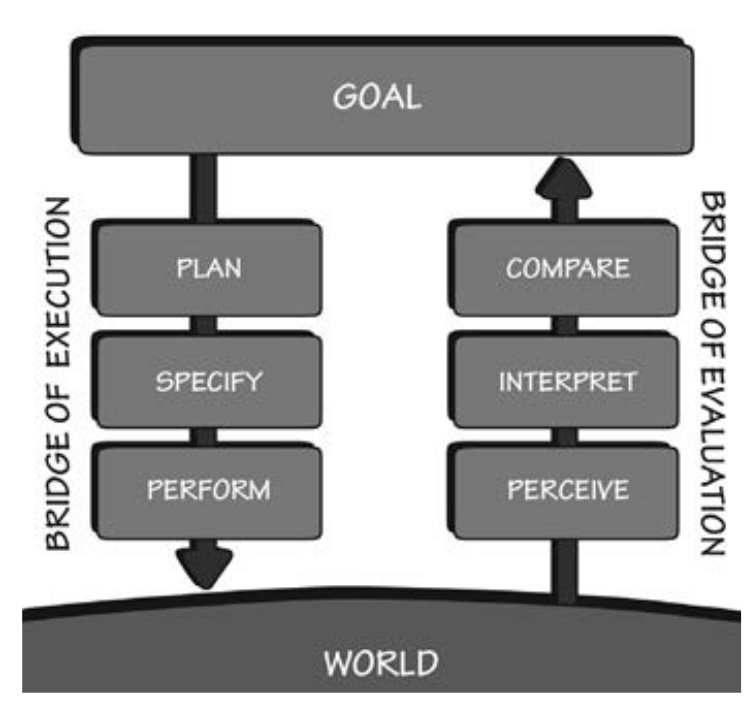
\includegraphics[width=0.5\textwidth]{figures/chapter1/Norman_7_stages_action.png}
\caption{The seven stages of actions defined by Norman \cite{norman2013design}. By giving a precise definition of each stage, this model guides the design and engineering of interactive systems by emphasizing each step of the cognitive processes taking place during an action. The designer can estimate the scope of the system and the potential errors at each stage of action.}
\label{fig:norman_7_stages}
\end{figure}

Indeed, too many systems require an expertise to be used. This often results from the system designer focusing on the ``machine part'' and not on the interface. Machines have been identified to avoid some humans flaws for a long time \cite{fitts_human_1951}, but because the ``interface'' \footnote{We refer here to the first meaning of ``interface'': the common surface where two systems meet and interact.} is too often poorly designed, the human needs to make great effort to use the machine. This effort becomes more important as the system gains in complexity and automation. This has been identified by Norman as the ``paradox of automation'' \cite{norman2013design}. More precisely, when an automation is performing a task the human situation awareness \cite{endsley_design_1988} decreases leading to misuses and errors when they need to interact with the system (\textit{e.g.} because of a system error or incapability).

\subsubsection{Human Robot Interaction}
When interacting with a robot, the human is no more the only agent taking autonomous decisions and able to act on the world. Indeed, not only the robot has its own plan-act-sense cycle with its own goal, but it can also physically move and change its environment. For the decision part, Bradshaw \textit{et al.} \cite{bradshaw2011human} propose eight maxims to complete and specify the recommendations of Norman. These maxims apply to human-agent interaction when they perform a joint activity:
\begin{itemize}
\item The agent must be \textit{observable}: its state and intentions are clearly exposed to others.
\item The agent must \textit{appraise progress}: it should inform others about the status of its task and warn them for any foreseen potential issues.
\item The agent must \textit{know its limits}: it should be proactive or wait when performing a task, depending on its evaluation of its capabilities.
\item The agent must be \textit{predictable} and \textit{dependable}: it should show what its capabilities are, and be trusted to use them at its best.
\item The agent must be \textit{directable}: its (sub)task can be preempted or modified if required and its knowledge can be updated thanks to other agents.
\item The agent must be \textit{selective}: it should expose only relevant facts in the context of the task.
\item The agent must be \textit{coordinated}: it should negotiate and deconflict plans, share resources and align beliefs between agents to create a \textit{common ground} if it is required to perform the task.
\end{itemize}

\unsure{I am afraid of adding thing here concerning the application of these things in task planning, I fear repetitions with "modeling human actions and shared plans...}

Interestingly, in their ``Architecture for autonomy'', Alami \textit{et al.} propose a robotic architecture which defines similar levels as the ones identified by Norman during human action \cite{alami1998architecture}.


% Focus on motion (navigation) => legibility, predictability, ...
Robot navigation should also respect these maxims. A number of approaches are trying to cope with these specific human robot issues \cite{kruse_human-aware_2013}. Moreover, more precise concepts have emerged from the maxims especially for the motion of a robot in a joint activity. 

First of all, the motion should ensure the physical safety of the surrounding humans. This is often respected by constraining the trajectory to stay at a minimal distance from humans \cite{kruse_human-aware_2013, rios2015proxemics}.

Moreover, while in a task, the motion of the robot can be used to convey information about its intentions, and thus making it more \textit{observable} and \textit{predictable}. Dragan \textit{et al.} defines three types of motions: functional, predictable and legible \cite{dragan2015effects}. A \textit{functional motion} is built only to make the robot move from on state to another one while avoiding humans and obstacles, it does not aim at providing any intent --- which does not mean it does not provide one. Then, a \textit{predictable motion} is a motion expected by an external observer knowing the robot model and its goal. It is often the quickest or shortest trajectory to reach the goal. Finally, a \textit{legible motion} is a motion allowing an external observer to quickly and reliably infer the robot motion goal.

However, as identified by Sisbot \textit{et al.}, to be identified as legible or predictable, the robot motion must be seen by the human. Accounting for the visibility of the robot by the human is paramount \cite{sisbot_human_2007}.  They integrate this constraint in a motion planner which is able to compute the safety of trajectories using the distance to a specified human and also prioritize visibility of the robot by estimating the field of view of the human and penalizing trajectories outside of it.

A lot of work has been made to generate legible paths. In \cite{beetz2010generality}, the robot learns usual motions from humans and generates trajectories based on them. However, even if the authors highlights the improvement in legibility, one could argue that the learned motions correspond more to the Dragan's definition of \textit{predictability}. In \cite{dragan_legibility_2013}, a robot motion planner is presented which is dedicated to generate legible trajectory. They prove its effectiveness through a user study while reporting an interesting finding: if the legibility of the motion is stressed to much, it becomes unpredictable and confuses the observer.




\subsection{Joint Action in Human-Robot Interaction}

Besides designing behaviors from scratch, previous work takes inspiration from situations where humans already perform a task with another autonomous agent: another human. Several previous contributions have been done studying how humans perform a so-called \textit{joint action}. \textit{Joint action} is defined by Sebanz \textit{et al.} as ``any form of social interaction whereby two or more individuals coordinate their actions in space and time to bring about a change in the environment'' \cite{sebanz2006joint}. Moreover, several work investigate multiple key abilities humans deploy when performing a joint action:
\begin{itemize}
\item humans can create and understand \textit{joint attention}: they are able to direct, or be directed by, others' attention \cite{pacherie_phenomenology_2011, sebanz2006joint}.
\item humans can \textit{predict} others' action effects and goals \cite{tomasello2005understanding, sebanz2006joint}.
\item humans can \textit{represent the shared task}: they can infer others' actions without directly seeing it, by observing events in the environment \cite{knoblich2011psychological, sebanz2006joint}.
\item humans can \textit{coordinate actions} by integrating others' actions into their own plan \cite{sebanz2006joint}.
\item humans consider combined actions results more important than their own only \cite{sebanz2006joint}.
\item yet, humans are able to \textit{distinguish their own actions from other's}, allowing them to find any divergence in beliefs or intentions and align them (\textit{e.g. through communication} if necessary \cite{pacherie_phenomenology_2011}.
\end{itemize}

Besides, a joint action can only occur if the involved agents know the presence of others agents but also their activity and intentions. Pacherie defines it as the mutual manifestness: ``\textit{each subject must be aware, in some sense, of the event as an event that is present to both; in other words the fact that both are attending to the same object or event should be open or mutually manifest}'' \cite{pacherie_phenomenology_2011}. Thus, it is not only necessary for the agents to account for the presence of the other but they also need to know they are involved in the same task.

Finally, studies show that humans can help the others to predict and coordinate their actions by communicating or slightly modifying their own. Coordination smoothers are defined as the changes in an agent own's behavior to ease the interaction with another one \cite{vesper_minimal_2010}.

It is interesting to note that some concepts are already overlapping with the desirable features for a robot taking part in an activity with a human. For example, the legibility and predictability of motion are based on models of the human capability to understand coordination smoothers and predict future actions effects. Bradshaw \textit{et al.} also refer to an ``extra work'' an agent has to perform to ensure an efficient interaction with a human partner \cite{bradshaw2003adjustable}, which can be linked to the mutual manifestness and the several mechanisms which can be used, and which a human expects, when interacting.

Moreover, some work already try to incorporate these joint action concepts and abilities into robotic architectures and behaviors \cite{khamassi2016integration, clodic2017key}. Lemaignan et al. present a robotic architecture composed of several components addressing the cognitive skills required to perform a collaborative task \cite{lemaignan2017artificial}. These include shared plan synthesis, human-aware motion planning --- both of which discussed later in this chapter ---, supervision, beliefs management and situation assessment. The situation assessment is able to generate symbolic facts from geometric data for the robot and also to estimate the beliefs of the human partner based on an estimation of their perspective of the scene \cite{milliez2014framework}. This framework has since been improved to a more modular approach allowing more refined reasoning, especially for the estimation of human beliefs \cite{lemaignan2018underworlds}. The supervision component is based on SHARY \cite{clodic2009shary} allowing the robot to execute shared plan while monitoring the human activities and deciding when to communicate. Devin \& Alami proposed an extended supervision system, heavily based on theory of mind, which is able to follow a shared plan but also to compute diverging agents beliefs, deciding if the divergence endangers the plan and if so, align the beliefs via verbal communications \cite{devin2016implemented}.

\section{Modeling Human Actions and Shared Plans}

It has been shown previously that a robotic agent interacting with a human needs to coordinate its actions with them. Moreover, joint action theory exhibits that humans interacting together are able to represent the task as a whole, and plan not only for their actions but also for the actions of other agents. Thus, we think that for a human to perform the most efficient and satisfactory joint task with a robot, this robot must explicitly model the human actions and plan not only for its actions but also for the human ones. In this part we will first introduce some notations used throughout all this thesis, then we will briefly show some ways of modeling human task and link them with robot task planning. Finally, we review some systems planning for both humans and robots when performing a joint task.

\subsection{Notations}
In order to help to differentiate between the models presented in this thesis, we introduce here some notations we will use in the thesis. These notations are partially inpired by from the work of Chakraborti \textit{et al.} \cite{chakraborti2018human}. We will refer to the model the robot has of itself as $\robotmodel$, to the model the robot has of the human it is interacting with as $\humanmodel$ and to the model the human has of the robot as $\robotinhumanmodel$. The models can represent different parts of the agent, ranging from their beliefs to their action model, while not being here a formal definition, the notation should help to understand to which agent we are referring to. It is important to note that all the components presented in this thesis are considered to be a part of the robot, and thus $\robotmodel$ plays a special role as we consider all the information in it as the ground truth. For example, if there is a belief divergence between $\robotmodel$ and $\humanmodel$, we always consider that the $\robotmodel$ is the truth, otherwise, it would make no sense to keep this information in $\robotmodel$ while having access to the one in $\humanmodel$.

\begin{figure}
\centering
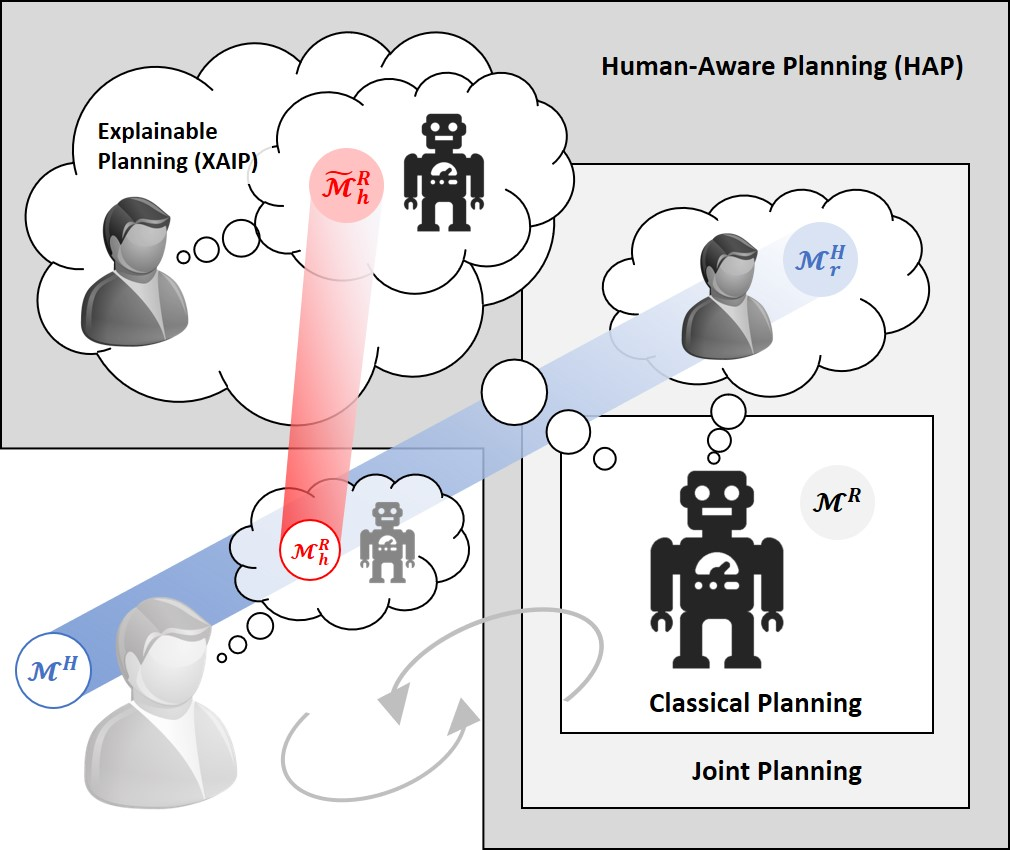
\includegraphics[width=0.7\textwidth]{figures/chapter1/chkraborti3models.png}
\caption{The notation coined by Chakraborti \textit{et al.} from \cite{chakraborti2018human} to represent the robot model $\robotmodel$, the estimated human model $\humanmodel$ and the estimated robot model the human has $\tilde{\robotinhumanmodel}$ (denoted $\robotinhumanmodel$ for simplicity as the real one is not accessible to the robot).}
\label{fig:chakraborti3models}
\end{figure}

\subsection{Task Modeling and Hierarchical Task Networks}
%, Hamster, Nau
\unsure{This part may be out of context here and probably shall be in Chapter4 only?}
\subsubsection{Human Task Modeling}
A common way of representing human activity ($\humanmodel$) and interaction with computer at high abstraction level is by using \textit{task models}. The hierarchical structure of human activity was first exploited by Annett and Duncan \cite{annett1967task}. They state that tasks can be described at several levels of abstraction until a certain criterion is met. Each task can thus be refined into subtasks detailing the procedure followed by the human to achieve the higher level task.
Task modeling has then evolved to introduce interaction with systems, produced and needed information, potential errors and a wide variety of operators specifying how tasks interacts with each other during their execution. Task models are now commonly used in user-centered and user interface designing processes. Most advanced notations include \textit{ConcurTaskTrees} \cite{paterno2004concurtasktrees} and \textit{HAMSTERS} \cite{martinie2019analysing}.
These models are used to design or to evaluate interactive systems. It allows the designer to better understand the user task or to study the user workflow using their system. However, these models contains to little information for a system to be able to reason and take decision on them (either in planning or acting).

\subsubsection{Robot Hierarchical Task Planning}
On the other hand, hierarchical representation of tasks are also used for decades in robotic planning ($\robotmodel$). In classical planning, each action of an agent is atomic and need some conditions to hold in the environment to be executed, then it changes the environment when applied. The planning process has then to find the right sequence of actions, being applicable one after the other to change the environment to reach a certain goal state. \acrfullpl{htn} allow the domain designer to help the plan search by inserting a hierarchy between these actions \cite{erol1996complexity}. Indeed, a network is composed of one or several tasks or actions, and each task has one or several decompositions. Each decomposition is itself a task network. The goal of the planner is not to find the sequence of actions to reach a goal, but rather to select recursively for each task the right decomposition ending (if possible) with a network of actions applicable from the initial state. Such a process is named by Ghallab, Nau and Traverso as \textit{planning with refinement methods} \cite{ghallab_nau_traverso_2016}.

This planning hierarchy not only allows the domain designer to guide the search by inserting some expertise into the model, but also to enhance explainability as the decompositions often offers a semantic to the subtask (the \textit{why} can usually be answered by going up in the hierarchy, while the \textit{how} is answered by going down).
% However used for evaluating or designing systems, but the system do not take decision based on it.
% Similar (hierarcical) HTN for robot planning... 

\subsection{Planning for Both the Human and the Robot}
%Charkrabori, Shah, HATP Jules, Epistemic planning?
While human activity modeling and autonomous planning have been studied separately for decades, there are still only few systems proposing to incorporate human activity into planning for intricate interactive tasks.
Planning for both a robotic agent and a human is not trivial. Indeed, while the robotic agent is planning for itself and will surely execute the plan, the human is not directly controllable (making them follow the plan may require the robot to at least communicate and perhaps negotiate) and can also has a plan themselves they are trying to execute.

The \acrfull{hatp} proposes a hierarchical approach to multi agent task planning \cite{alili2009task, lallement2014hatp}. This \acrshort{htn} based planner is able to elaborate a multi agent plan based on a single \acrshort{htn} tree (unifying both $\robotmodel$ and $\humanmodel$). Moreover, it maintains one belief base per agent allowing to write task decomposition rules and actions preconditions and effects in any agent belief base. Finally, \acrshort{hatp} also computes costs for the found plans based on action costs and predefined social rules. More details about HATP will be presented in Chapter~\ref{chapter:comm}. This task planner has been coupled with the Geometrical Task Planner (GTP) allowing to also plan the geometrical motion of the human partner to inform HATP about the feasibility and the cost of a motion action \cite{gharbi2015combining}. As stated before, HATP has been used in complete robotic architecture \cite{devin2016implemented, lemaignan2017artificial}.

Buckingham \textit{et al.} propose a planning scheme questioning humans mental models ($\humanmodel$) returning the effects of expected future humans actions \cite{buckingham2020robot}. The planner is then able to determine a robot policy ($\robotmodel$) influencing the humans actions. In this work, they show how this framework is able to cope with interactive tasks even without assuming that the human is collaborating.

Similarly, Unhelkar \textit{et al.} proposed a POMDP-based approach called CommPlan \cite{unhelkar2020decision}. The POMDP is built using a user defined MDP (Markov Decision Process) representing the collaborative task and an AMM (Agent Markov Model) to represent the human decision-making process ($\humanmodel$). This POMDP is then solved to produce a robot policy ($\robotmodel$) which, in particular, decides when the robot has to communicate about its beliefs, to question the human about theirs and to ask the human to perform an action. Besides, the human AMM ($\humanmodel$) is not only specified by the programmer but also refined during the interaction via learning.

Besides, to cope with the uncertainty of the human knowledge ($\humanmodel$), Petrick and Foster propose to use conditional planning allowing to plan for incomplete information~\cite{petrick2013planning}. By doing so, the planner elaborates a plan for the robot ($\robotmodel$) accounting for multiple possible human choices, and depending on the knowledge received the execution component can execute the right branch of the plan.

Likewise, Sanelli \textit{et al.} (\cite{sanelli2017short}) present an approach not only elaborating conditional plans for the robot ($\robotmodel$)  depending on the possible human choices ($\humanmodel$, \textit{e.g.} the choice of activity the human wants to perform), but they are able to transform this conditional plan into a Petri net plan to handle its execution. This contribution is inspired from a previous work by Nardi and Iocchi (\cite{nardi2014representation}) in which they present a method for transforming (linear) joint plan (both $\robotmodel$ and $\humanmodel$) into a Petri net plan managing its execution. Interestingly, the human actions from the plan are changed into a part of the Petri net where the robot elicit the action (\textit{e.g.} via a verbal communication) if the human does not perform it by themselves. However, this approach only request the human to make single actions, instead of sharing a high level goal, which can become unpleasant if done repeatedly. 

Chakraborti \textit{et al.} uses both the robot model ($\robotmodel$) and the estimation of the model the human has of the robot ($\robotinhumanmodel$) to improve plan explicability \cite{chakraborti2017plan}. Indeed, they propose a novel approach called model reconciliation which they present as a classical planning problem. In this problem, the goal is to make identical the both optimal plans generated via the robot model $\robotmodel$ and the human estimation of the robot model $\robotinhumanmodel$. To do so, they define a list of operators on the models in order to modify them until the plans matches. To our knowledge it is the only approach both reasoning on $\robotinhumanmodel$ and operating directly on the action models. However, it only has been applied to robot plans and not to joint plans. Indeed, the plans generated contain robot actions only, and the robot and the human do not directly collaborate in the presented tasks.

% Geometrical collabortaive planning (HATEB, Jules)
Geometrical planning in human robot activity has also been studied in several works. For navigation, Khambhaita and Alami proposed a planner which optimizes both the human and the robot trajectories ($\robotmodel$ and $\humanmodel$) \cite{khambhaita_viewing_2017}. This allows the robot not only to have a prediction of the human future trajectory, but also to model their interactions and how its own trajectory can affect the human's one. The approach will be detailed in Chapter~\ref{chapter:navigation}.

Besides, representing humans as a group has also been showed as beneficial for robot navigation. For instance, for the robot-waiters problem, where multiple robots compute trajectories in order to serve multiple moving humans in a room containing obstacles, Saraydaryan \textit{et al.} (\cite{saraydaryan2015robots}) showed that considering clusters of humans to be served allows to decrease the human idleness (the duration for which a human has not been served by a robot). These humans clusters are called F-Formations when the human are actively interacting with each other in the cluster (\textit{e.g.} a group of human discussing together). Recognizing them and integrating them ($\humanmodel$) in the robot trajectory computation ($\robotmodel$) in order to socially integrate them or to not disturb them also allows for more acceptable robot trajectories (\cite{althaus2004navigation}).

Another work presents a motion planner allowing to balance the effort between the robot and the human, depending on the mobility of the human, for a handover task \cite{mainprice2012sharing}. To do so, they sample an acceptable position for the human ($\humanmodel$) according to several parameters, including its settable mobility, then they try to plan a trajectory for both the robot ($\robotmodel$) and the human ($\humanmodel$) to get them into an handover configuration. This work has then be extended and generalized by Waldhart, Gharbi and Alami to handle several robots and humans \cite{waldhart2015planning}.

Finally, Waldhart, Clodic and Alami proposed a geometric planner, able to find the best robot and human positions for the robot to point a landmark at the human \cite{waldhart_reasoning_shared_2019}. This planner uses the human vision ability and mobility ($\humanmodel$) as well as robot mobility and respect of a pointing triangle formation between the robot, the human and the landmark to point ($\robotmodel$).

From all these contributions we see a great interest in planning for both the human and the robot. Indeed, they allow to represent multiple features highly desired in human robot interaction scenarios. First, by planning for both, shared goals and coordinated actions can be represented. The planners are able to elaborate plans (or trajectories) that do not conflict between the agents, and even that interact in a collaborative way to reach the shared goal. 

Then, it allows to attribute tasks to either one agent or the other if they can be done by both. Unlike other task attribution approaches, modeling the human helps to estimate the effort taken in the contribution of the joint plan. The planner can ensure that most of the effort is taken by the robot but can also balance other solutions depending on the context (\textit{e.g.} urgency to perform the task, where the human may accept to contribute more to do it faster). 

Finally, when integrated in a robotic architecture and in a real human robot scenario, planning for both reveals to be key. Indeed, planning before acting usually avoids deadlocks during execution or sub-optimal solutions which would have been encountered by only reasoning on short term. But for human robot interaction it also allows to estimate the effort and the contribution of each agent \textit{before involving the human}. Moreover, the resulting joint plan can then be negotiated with the human before starting the task, allowing for a better efficiency, satisfaction, explainability and acceptability.

Not all of these challenges have been entirely tackled yet. In this thesis we propose to explore multiple ways of planning for both agents. 

\ifdefined\included
\else
\bibliographystyle{acm}
\bibliography{These}
\end{document}
\fi


\ifdefined\included
\else
\documentclass[a4paper,11pt,twoside]{StyleThese}
\usepackage{amsmath,amssymb, amsthm}             % AMS Math
\usepackage[T1]{fontenc}
\usepackage[utf8x]{inputenc}
\usepackage{babel}
\usepackage{datetime}

\usepackage{silence}

\WarningFilter{minitoc(hints)}{W0023}
\WarningFilter{minitoc(hints)}{W0028}
\WarningFilter{minitoc(hints)}{W0030}

\usepackage{lmodern}
\usepackage{tabularx}
%\usepackage{tabular}
\usepackage{multirow}
\usepackage{xspace}

\usepackage{hhline}
\usepackage[left=1.5in,right=1.3in,top=1.1in,bottom=1.1in,includefoot,includehead,headheight=13.6pt]{geometry}
\renewcommand{\baselinestretch}{1.05}

% Table of contents for each chapter

\usepackage[nottoc, notlof, notlot]{tocbibind}
\usepackage{minitoc}
\setcounter{minitocdepth}{2}
\mtcindent=15pt
% Use \minitoc where to put a table of contents

\usepackage{aecompl}

% Glossary / list of abbreviations

\usepackage[intoc]{nomencl}
\iftoggle{ThesisInEnglish}{%
\renewcommand{\nomname}{Glossary}
}{ %
\renewcommand{\nomname}{Liste des Abréviations}
}

\usepackage{etoolbox}
\renewcommand\nomgroup[1]{%
  \item[\bfseries
  \ifstrequal{#1}{A}{Number Sets}{%
  \ifstrequal{#1}{G}{Agents Beliefs and Action Models}{%
  \ifstrequal{#1}{N}{Navigation}{%
  \ifstrequal{#1}{O}{Ontology}{%
  \ifstrequal{#1}{R}{Referring Expression Generation}{%
  \ifstrequal{#1}{Z}{Controllable and Uncontrollable Agents Task Planning}{}}}}}}%
]}

\makenomenclature



% My pdf code

\usepackage{ifpdf}

\ifpdf
  \usepackage[pdftex]{graphicx}
  \DeclareGraphicsExtensions{.jpg}
  \usepackage[pagebackref,hyperindex=true]{hyperref}
  \usepackage{tikz}
  \usetikzlibrary{arrows,shapes,calc}
\else
  \usepackage{graphicx}
  \DeclareGraphicsExtensions{.ps,.eps}
  \usepackage[dvipdfm,pagebackref,hyperindex=true]{hyperref}
\fi

\graphicspath{{.}{images/}}

%% nicer backref links. NOTE: The flag ThesisInEnglish is used to define the
% language in the back references. Read more about it in These.tex

\iftoggle{ThesisInEnglish}{%
\renewcommand*{\backref}[1]{}
\renewcommand*{\backrefalt}[4]{%
\ifcase #1 %
(Not cited.)%
\or
(Cited in page~#2.)%
\else
(Cited in pages~#2.)%
\fi}
\renewcommand*{\backrefsep}{, }
\renewcommand*{\backreftwosep}{ and~}
\renewcommand*{\backreflastsep}{ and~}
}{%
\renewcommand*{\backref}[1]{}
\renewcommand*{\backrefalt}[4]{%
\ifcase #1 %
(Non cité.)%
\or
(Cité en page~#2.)%
\else
(Cité en pages~#2.)%
\fi}
\renewcommand*{\backrefsep}{, }
\renewcommand*{\backreftwosep}{ et~}
\renewcommand*{\backreflastsep}{ et~}
}

% Links in pdf
\usepackage{color}
\definecolor{linkcol}{rgb}{0,0,0.4} 
\definecolor{citecol}{rgb}{0.5,0,0} 
\definecolor{linkcol}{rgb}{0,0,0} 
\definecolor{citecol}{rgb}{0,0,0}
% Change this to change the informations included in the pdf file

\hypersetup
{
bookmarksopen=true,
pdftitle="Planning For Both Robot and Human: Anticipating and Accompanying Human Decisions",
pdfauthor="Guilhem BUISAN", %auteur du document
pdfsubject="Thèse", %sujet du document
%pdftoolbar=false, %barre d'outils non visible
pdfmenubar=true, %barre de menu visible
pdfhighlight=/O, %effet d'un clic sur un lien hypertexte
colorlinks=true, %couleurs sur les liens hypertextes
pdfpagemode=None, %aucun mode de page
pdfpagelayout=SinglePage, %ouverture en simple page
pdffitwindow=true, %pages ouvertes entierement dans toute la fenetre
linkcolor=linkcol, %couleur des liens hypertextes internes
citecolor=citecol, %couleur des liens pour les citations
urlcolor=linkcol %couleur des liens pour les url
}

% definitions.
% -------------------

\setcounter{secnumdepth}{3}
\setcounter{tocdepth}{2}

% Some useful commands and shortcut for maths:  partial derivative and stuff

\newcommand{\pd}[2]{\frac{\partial #1}{\partial #2}}
\def\abs{\operatorname{abs}}
\def\argmax{\operatornamewithlimits{arg\,max}}
\def\argmin{\operatornamewithlimits{arg\,min}}
\def\diag{\operatorname{Diag}}
\newcommand{\eqRef}[1]{(\ref{#1})}

\usepackage{rotating}                    % Sideways of figures & tables
%\usepackage{bibunits}
%\usepackage[sectionbib]{chapterbib}          % Cross-reference package (Natural BiB)
%\usepackage{natbib}                  % Put References at the end of each chapter
                                         % Do not put 'sectionbib' option here.
                                         % Sectionbib option in 'natbib' will do.
\usepackage{fancyhdr}                    % Fancy Header and Footer

% \usepackage{txfonts}                     % Public Times New Roman text & math font
  
%%% Fancy Header %%%%%%%%%%%%%%%%%%%%%%%%%%%%%%%%%%%%%%%%%%%%%%%%%%%%%%%%%%%%%%%%%%
% Fancy Header Style Options

\pagestyle{fancy}                       % Sets fancy header and footer
\fancyfoot{}                            % Delete current footer settings

%\renewcommand{\chaptermark}[1]{         % Lower Case Chapter marker style
%  \markboth{\chaptername\ \thechapter.\ #1}}{}} %

%\renewcommand{\sectionmark}[1]{         % Lower case Section marker style
%  \markright{\thesection.\ #1}}         %

\fancyhead[LE,RO]{\bfseries\thepage}    % Page number (boldface) in left on even
% pages and right on odd pages
\fancyhead[RE]{\bfseries\nouppercase{\leftmark}}      % Chapter in the right on even pages
\fancyhead[LO]{\bfseries\nouppercase{\rightmark}}     % Section in the left on odd pages

\let\headruleORIG\headrule
\renewcommand{\headrule}{\color{black} \headruleORIG}
\renewcommand{\headrulewidth}{1.0pt}
\usepackage{colortbl}
\arrayrulecolor{black}

\fancypagestyle{plain}{
  \fancyhead{}
  \fancyfoot{}
  \renewcommand{\headrulewidth}{0pt}
}

%\usepackage{MyAlgorithm}
%\usepackage[noend]{MyAlgorithmic}
\usepackage{algorithm}
\usepackage[noend]{algpseudocode}
\usepackage{comment}
\usepackage[ED=EDSYS-Robo, Ets=INSA]{tlsflyleaf}
%%% Clear Header %%%%%%%%%%%%%%%%%%%%%%%%%%%%%%%%%%%%%%%%%%%%%%%%%%%%%%%%%%%%%%%%%%
% Clear Header Style on the Last Empty Odd pages
\makeatletter

\def\cleardoublepage{\clearpage\if@twoside \ifodd\c@page\else%
  \hbox{}%
  \thispagestyle{empty}%              % Empty header styles
  \newpage%
  \if@twocolumn\hbox{}\newpage\fi\fi\fi}

\makeatother
 
%%%%%%%%%%%%%%%%%%%%%%%%%%%%%%%%%%%%%%%%%%%%%%%%%%%%%%%%%%%%%%%%%%%%%%%%%%%%%%% 
% Prints your review date and 'Draft Version' (From Josullvn, CS, CMU)
\newcommand{\reviewtimetoday}[2]{\special{!userdict begin
    /bop-hook{gsave 20 710 translate 45 rotate 0.8 setgray
      /Times-Roman findfont 12 scalefont setfont 0 0   moveto (#1) show
      0 -12 moveto (#2) show grestore}def end}}
% You can turn on or off this option.
% \reviewtimetoday{\today}{Draft Version}
%%%%%%%%%%%%%%%%%%%%%%%%%%%%%%%%%%%%%%%%%%%%%%%%%%%%%%%%%%%%%%%%%%%%%%%%%%%%%%% 

\newenvironment{maxime}[1]
{
\vspace*{0cm}
\hfill
\begin{minipage}{0.5\textwidth}%
%\rule[0.5ex]{\textwidth}{0.1mm}\\%
\hrulefill $\:$ {\bf #1}\\
%\vspace*{-0.25cm}
\it 
}%
{%

\hrulefill
\vspace*{0.5cm}%
\end{minipage}
}

\let\minitocORIG\minitoc
\renewcommand{\minitoc}{\minitocORIG \vspace{1.5em}}

\usepackage{multirow}
%\usepackage{slashbox}

\newenvironment{bulletList}%
{ \begin{list}%
	{$\bullet$}%
	{\setlength{\labelwidth}{25pt}%
	 \setlength{\leftmargin}{30pt}%
	 \setlength{\itemsep}{\parsep}}}%
{ \end{list} }

\theoremstyle{definition}
\newtheorem{definition}{Definition}
\renewcommand{\epsilon}{\varepsilon}

% centered page environment

\newenvironment{vcenterpage}
{\newpage\vspace*{\fill}\thispagestyle{empty}\renewcommand{\headrulewidth}{0pt}}
{\vspace*{\fill}}

\usepackage{tablefootnote}

\theoremstyle{plain}
\newtheorem{constraint}{Constraint}[section]

\algnewcommand\algorithmicforeach{\textbf{for each}}
\algnewcommand\algorithmicin{\textbf{in}}
\algdef{S}[FOR]{ForEach}[2]{\algorithmicforeach\ #1\ \algorithmicin\ #2\ \algorithmicdo}

\usepackage{listings}
\lstdefinestyle{customPlan}{
  language=C,
  commentstyle=\itshape\color{green!25!black},
}
\usepackage{pdfpages}

\sloppy
\begin{document}
\setcounter{chapter}{1} %% Numéro du chapitre précédent ;)
\dominitoc
\faketableofcontents
\fi

\chapter{Coplanning for navigation}
\minitoc

\section{Introduction}
In a lot of human robot interaction scenarios, the robot has to move in the environment to accomplish its task. It can either be that the task cannot be done in the direct vicinity of the robot or that the task itself is to move elsewhere. For example in the MuMMER project, a Pepper robot in a mall has to give direction instructions to guide a human to their wanted location. The robot is also able to point to visible landmarks to locate the beginning of the route (\textit{e.g.} saying \textit{"Take these stairs, then take the corridor on your right and the shop will be on your left" while pointing to the stairs}). However, some obstacles in the proximity of the robot and the guided human can prevent them to see the pointed landmarks, or a corridor crossing can be hidden, making the route description one step longer than it should be. Thus, to perform the task of route guiding more efficiently, the robot might decide to move.
In the Spencer project, another robot has to guide people to their gate in the Schipol airport. Here, the robot will navigate all the way from the starting point to the final destination while ensuring the human is actually following it, but also has to avoid other pedestrians. In this example, the navigation of the robot is a main part of the task.
In both example, the robot has to make plan its motion such as the physical and psychological safety of surrounding humans are ensured. However, not taking into account the motion of these humans during the planning process may lead to suboptimal trajectories or even deadlock.
We propose in this chapter to, after a survey of related works, present a navigation planner algorithm taking into account both the robot and the human, then to show how this approach can be used to enhance mutual manifestness and improve efficiency in a narrow corridor crossing scenario through a user study, and finally report some extension made to the approach to include humanoid robots, flying drone and to estimate the progression of the navigation task. 

\section{Related Work}
\subsection{Human-Aware Robot Navigation}
The aim of robot navigation is to make the robot base move from one place to another while avoiding static and moving obstacles. However, when the robot has to move in an environment where humans are evolving other constraints must be added. The robot must not only avoid the humans, as any other moving obstacle, to ensure their physical safety (not harming them), but also take into account their psychological safety (not stressing or frightening them) \cite{sisbot_human_2007}, \cite{kruse_human-aware_2013}. In order to respect these constraints several methods have been used. The first largely used is based on costmap exploration. Based on the robot known humans and obstacles in the environment a grid is built, where each cell has a cost representing places the robot should avoid to pass through. Then, given a start and an end points, a planner can explore this grid and try to minimize the cost along the trajectory (\cite{sisbot_human_2007}, \cite{lu_towards_2013}). These approaches are usually pretty efficient but since a whole grid can take time to compute, they can perform poorly in dynamic environments.

Another approach is to use the social force model \cite{helbing_social_1995}. A robot trajectory is computed based on repulsive or attractive force fields set on humans, obstacles and goal \cite{ferrer_robot_2013}. This gives good results in open environments but the trajectories can be erratic in confined environment with a lot of obstacles and humans because of the diverging "forces" applied. Moreover, by only considering the robot plan, these planners return no solution if the robot and the human must cross each other in a narrow corridor where the human is centered leaving no place for the robot to go. This is why we need a planner able to \textit{infer} that the human can move to one side of the corridor allowing the robot to cross on the other side.

In their work, Kuderer et al. use social force model to both compute the robot trajectories and predict the nearby human ones \cite{kuderer_feature-based_2012}. However, the resulting human trajectories are more reactions to robot motion than coplanning solutions.

To overcome this limitation, Khambhaita \& Alami proposed a navigation planner based on an optimization scheme. In this approach the trajectories of the robot and of the nearby humans are optimized together at real time to create, at position control rate, a conavigation solution \cite{khambhaita_viewing_2017}. This ensures that at all time it exists for the humans a solution to go to their known goal, and that this solution is optimal regarding a different set of constraint based on human models.

Although, even if the robot computes an optimal solution for the human and itself, it is pointless if it cannot communicate or show this solution to the human (\textit{e.g.} either it plans to go to the left or the right of the corridor, so the human can either accept or decline this plan). Thus, the robot must also try to make its intention clear \cite{pacchierotti_evaluation_2006}. This ability of a robot to exhibit its future actions is called legibility. A legible robot will have its future actions and goals inferred quicker \cite{dragan_legibility_2013}, which is crucial in entangled tasks such as crossing in a narrow corridor. For navigation, legibility can be increased either by changing the robot speed along the trajectory \cite{kruse_legible_2012} or by modifying its trajectory \cite{khambhaita_viewing_2017}.

In a broader sense, the changes in an agent's own behavior in order to make easier the interaction with another agent are called coordination smoothers \cite{vesper_minimal_2010}. We claim that a robot should exhibit some coordination smoothers when interacting with a human to increase its usability. Moreover, all the coordination smoothers are not equal, as some can bring more information thant other. A simple blinking light and beeping sound when the robot is moving are conveying less information than turn signals for example. In our case, since we deal with anthropomorphic robots, we can try to make even more efficient coordination smoothers by using what can be identified as the head of the robot.

\subsection{Communicating Intents Via the Robot Gaze} \unsure{Cette subsection n'a peut-être rien à faire ici...}
Some robots have a movable part that can be identified as an head, and often contains camera or similar devices that can be recognized eyes. the resulting robot \textit{gaze} has already been used to effectively increase the user attention and engagement \cite{mutlu_storytelling_2006}, \cite{zaraki_designing_2014}. Moreover, the robot gaze has also been shown useful in navigation to indicate turning intentions \cite{lu_towards_2013}, \cite{may_show_2015}, and thus increase legibility.

Besides, in intricate collaborative activities, each agent must show to the other one that they are aware of their presence and actions. Pacherie defines it as the mutual manifestness: \textit{each subject must be aware, in some sense, of the event as an event that is present to both; in other words the fact that both are attending to the same object or event should be open or mutually manifest} \cite{pacherie_phenomenology_2011}. Thus, it is interesting to know if in intricate human robot navigation tasks, making the robot show mutual manifestness increase the efficiency of the task.



\section{The Human Aware Timed Elastic Band}
The only work to our knowledge being able to, in real time, plan trajectories for the robot and the humans surrounding it, is the \textit{Human Aware Timed Elastic Band} \cite{khambhaita_viewing_2017}. Thus, we used it as the backbone of our work, and made several contributions around it.

\subsection{General scheme}
The human aware timed elastic band algorithm is based on the timed elastic band (TEB) approach from Rosmann et al. \cite{rosmann_efficient_2013}. This approach is a local optimization problem where the successive positions $(x_i, y_i) \in \realset$ and orientations $\theta_i \in S^1$ of the robot along with the time steps $\Delta T_i \in \realset$ between each consecutive poses are optimized to minimize a multi criteria cost function up to a fixed length horizon $n \in \intset$. To put it otherwise, the elastic band trajectory of the robot is represented by its poses: 
\[Q = \{\textbf{s}_i\}_{i=0..n} with \textbf{s}_i = [x_i, y_i, \theta_i]^T\] to which are added the time intervals between two consecutive poses: \[\tau = {\Delta T_i}_{i=0..n-1}\] Resulting in the \textit{time elastic band} \[B := (Q, \tau)\] having to be optimized to minimize the cost function $f(B)$ to get the optimal trajectory \[B^* = \mathop{\mathrm{argmin}}_B\,f(B)\]
This function takes the form of a multi criteria weighted sum cost function which can be rewritten as: \[ f(B) = \sum_{k} \gamma_k f_k(B) \] where $\gamma_k \in \realset$ are weights allowing the designer to balance the importance between cost functions $f_k$.

This planner has been integrated has a local planner in the ROS architecture. Provided with a global plan (often generated with an A* algorithm) of the long trajectory, the local planner generates short term plans (up to several meters), avoiding static and dynamic obstacles (both known by the global planner and discovered with the robot sensor during the navigation) and minimizing the trajectory duration. In addition, the local planner is responsible for generating the speed command at position control rate (around 10 Hz usually). TEB does it by optimizing the local trajectory and computing the wanted robot speed from the first two poses and the time interval between them. Moreover, if the optimization process takes too long, the length horizon of the global trajectory on which the local optimization is performed is reduced, and increased if the optimization time is satisfactory.

In the human aware timed elastic band approach, multiple timed band are considered. In addition to the robot band $\robotband$ represents the robot trajectory, it also considers multiple human bands $B_{\mathcal{H}_k}$ with $k in \intset$ the number of humans in vicinity of the robot. For simplicity purpose, in this thesis we will only consider one human in the vicinity of the robot, and thus one human band $\humanband$. However, the approach has been shown working successfully up to three humans.
Moreover, the weighted-sum cost function becomes:
\begin{equation} \label{eq:hateb_obj_function}
f(\robotband, \humanband) = \sum_a \gamma_a f_a(\robotband) + \sum_b \gamma_b f_b(\humanband) + \sum_c \gamma_c f_c(\robotband, \humanband)
\end{equation}   

where $fa$, $fb$ and $fc$ represent respectively cost functions associated with robot trajectory constraints, human trajectory constraints and human-robot social constraints. Then, the optimization process consist in finding the optimal robot and human trajectories $\robotband, \humanband$ such as:
\[\{\robotband^*, \humanband^*\} = \mathop{\mathrm{argmin}}_{\{\robotband, \humanband\}}\,f(\robotband, \humanband)\]





\subsection{Constraints}
In this optimization scheme, all the constraints are represented as cost in the function. Thus, there is no \textit{hard constraints}, but using the weight of each one, we are able to prioritize some over the others. Moreover, when a trajectory has been optimized, before being executed, the local planner checks that it respects all the defined hard constraints (kinodynamic constraints and obstacles separation).

The new formulation of Khambhaita et al. allows to separate the constaints into three categories:
\begin{itemize}
\item Robot trajectory constraints: these constraints represent the robot kinodynamic constraints (non holonomic, maximum speed, maximum acceleration) as well as preventing the robot trajectory to differ too much from the global plan. They are presented in \cite{rosmann_efficient_2013}.
\item Human trajectory constraints: these constraints represent the human kinodynamic constraints and prevent them to differ too much from the global trajectory. They are the same as the robot ones, but their parameters (\textit{e.g.} maximum speed threshold) must not be set by the designer but evaluated by the robot during the evaluation.
\item Human-robot social constraints: these constraints represent how the human and robot trajectory must interact with each other. Khambhaita et al. presneted the \textit{safety} constraint, ensuring a sufficient distance between the robot and the human; the \textit{directional constraint} discouraging trajectories where the robot and the human move straight to each other; and the \textit{time-to-collision} (TTC) constraint, preventing the robot and the human to adopt speed which, if maintained, would lead to a collision. The latter will be detailed in what follows as it was studied more in depth through a user study.
\end{itemize}

It worth noting that different weights can be set for each constraint, and that they can be adjusted dynamically during the navigation. Moreover, by setting different weight between the robot and the human for the constraint preventing to move away from the global plan, we can adjust the \textit{stiffness} of the trajectories, thus allowing one agent or the other to elongate their trajectory, taking more or less effort into the collaborative navigation.

\section{Evaluating enhanced mutual manifestness in a crossing scenario}
In this section we present an user study aiming at assessing the pertinence of using a conavigation planner in a situation where a human and a robot must cross each other in a narrow corridor. This task of crossing in narrow corridor is challenging as both agents start in the center of either end of the corridor, and there is no way for one agent to find a way if the other agent does not move to the other side. Thus, we state that not only coplanning is required to find a plan reaching the other end of the corridor (by planning that the other agent will also cooperate and move on one side), but showing intentions and awareness of the other agent is crucial for the interaction to unfold without trouble.

\subsection{Robot behavior design}
For this user study we were particularly interested in finding if and how navigation coplanning would lead to higher mutual manifestness and to higher efficiency in crossing.
To do so, we designed a robot behavior using the HATEB navigation planner.
In their work Kambhaita et al. showed that during a narrow crossing the robot is able to plan that the human and the robot will choose opposite sides of the corridor. But if the robot shows its plan when it faces the human, they would have little time to react, and might also move to the same side as the robot, needing negotiation and replanning, reducing the overall efficiency of the crossing. The robot must thus, show the plan (\textit{i.e.} the plan trajectory, or here, the side of the corridor it plans to take) early in the crossing.
By reducing the TTC constraint function threshold and increasing its weight, we discourage trajectories where the robot and the human are facing each other. Thus, if the robot trajectory stiffness is lower than the human one, the robot will move to the chosen side of the corridor early in the trajectory as shown in Fig.~\ref{ttc_explanations}.


\begin{figure}[hbtp]
\centering
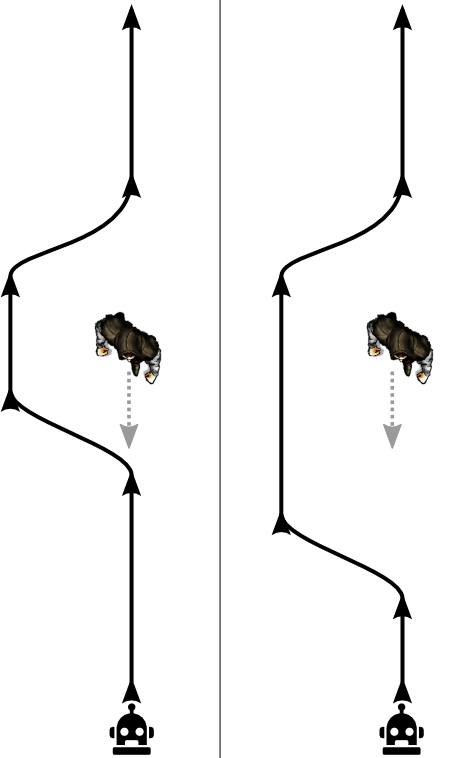
\includegraphics[scale=0.4]{figures/chapter2/condition_1_proactivity_shrink.png}
\caption{Influence of the modification of the TTC constraint cost weight on the trajectory. On the left, the weight is low, the robot will show the side and avoid the human at the last moment. On the right, the weight is high, the robot will show the chosen side and avoid the human much earlier.}
\label{ttc_explanations}
\end{figure}

Moreover, as stated before \unsure{maybe move the gaze stuff from related work to here?} several papers show that using the \textit{head} of a robot can significantly improve legibility and mutual manifestness. Thus, we also chose to make the robot look at its future planned trajectory as shown in Fig.~\ref{head_gaze_behavior}. This is possible thanks to the HATEB algorithm which, unlike many other local planner only publishing  speed commands \improvement{Adds ref to DWA for example ?}, also publishes a precise short-term trajectory. Finally, to show the robot awareness of the human presence, we made it \textit{glance} at the human twice when they enter a large and a small radius circle.

\begin{figure}[hbtp]
\centering
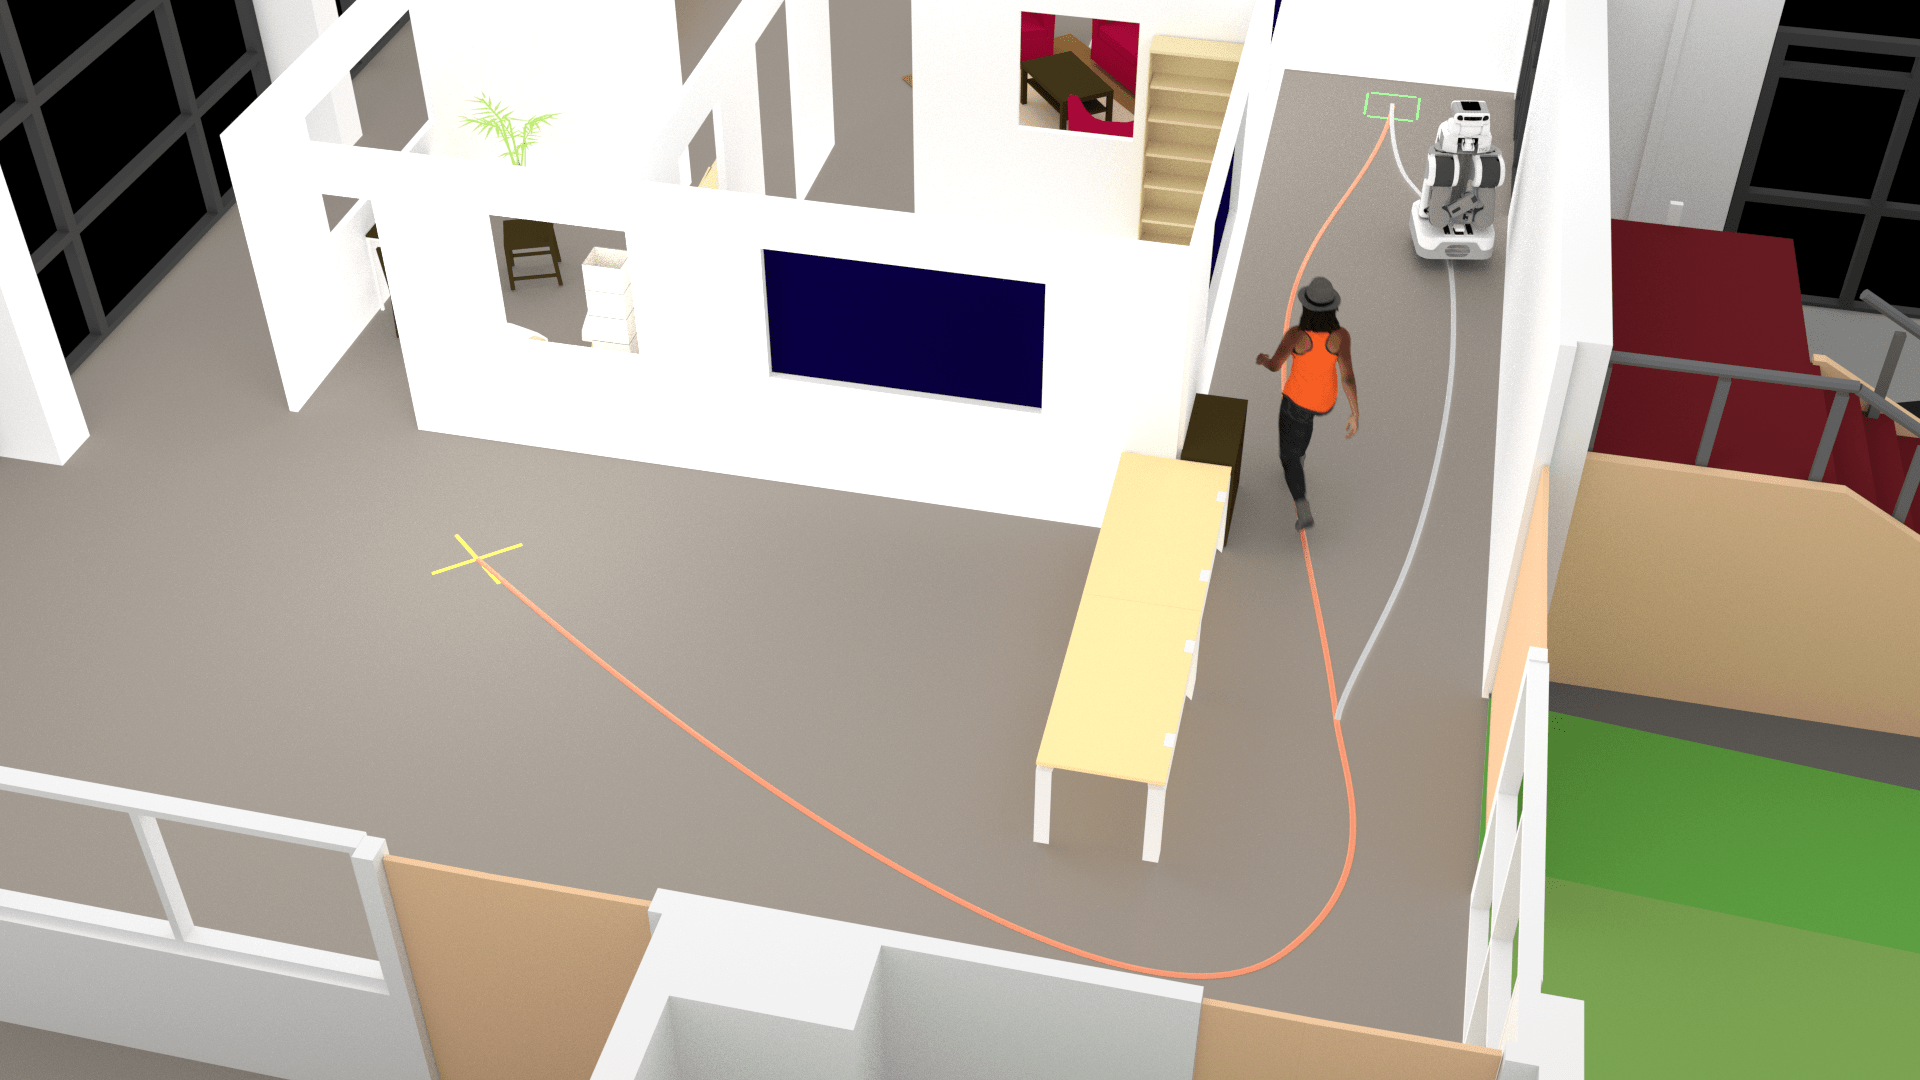
\includegraphics[scale=0.4]{figures/chapter2/expe_human-min.png}
\caption{Behavior implemented for the robot head. The robot \textit{looks} at a point placed at its planned position X seconds in the future and h meters above the ground.}
\label{experiment_adream}
\end{figure}

\subsection{User study protocol}

\begin{figure}[hbtp]
\centering
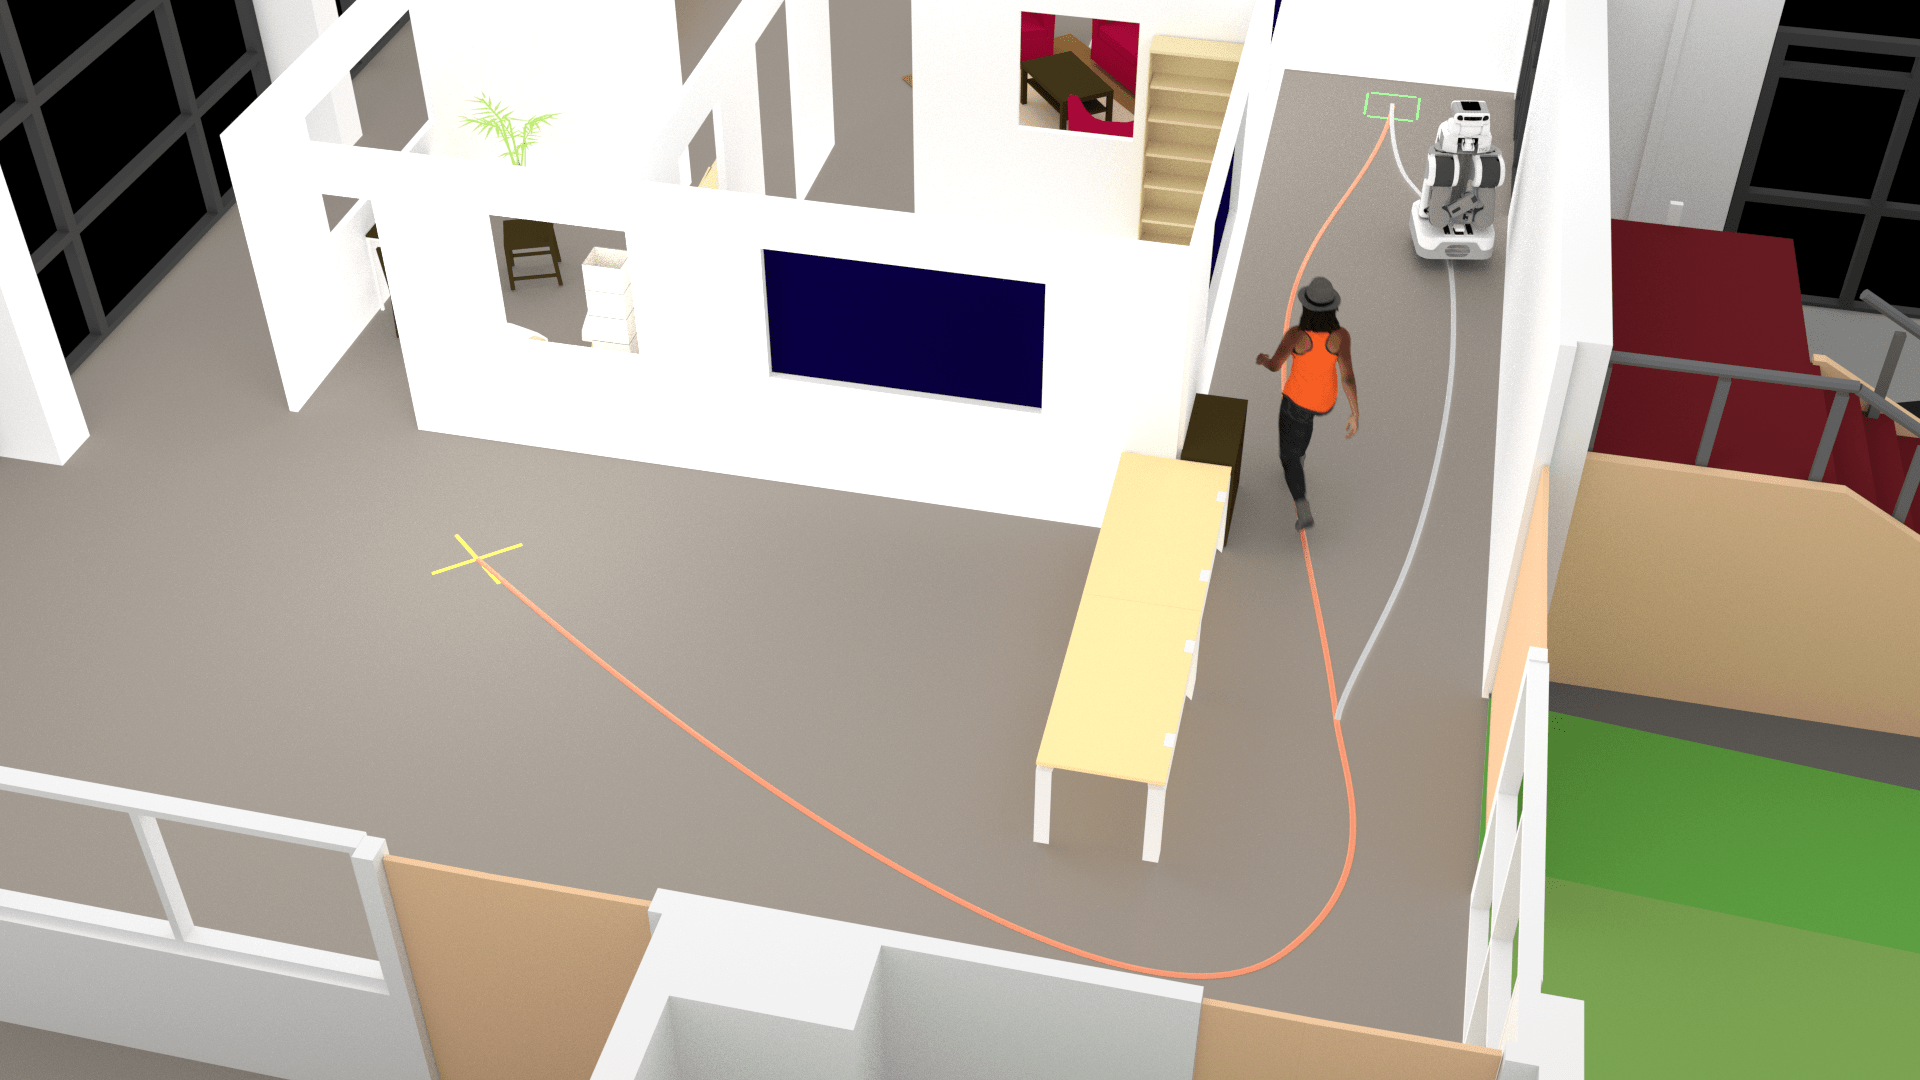
\includegraphics[scale=0.4]{figures/chapter2/expe_human-min.png}
\caption{The  study  environment.  The  participant  had  to  go  from  the  yellow  cross  marked  on  the  ground  to  the  green  square  also  marked  on  the  ground,which was the robot starting point. Crossing occurred roughly in the area where the robot and participant are on the picture. Trajectories are displayed on the picture for example only and where not marked on the ground or suggested by the experimenters at any time.}
\label{head_gaze_behavior}
\end{figure}

\subsubsection{Objective}
The aim of this study is to evaluate the impact of the TTC cost constraint and head behavior on usability. We designed an user study where actual individuals have to walk through a corridor facing a fully autonomous navigating robot. The afore-explained robot behavior was used. We measured the quality of the interaction between the robot and the human with both objective (visual behavior) and subjective data. The subjective evaluation was based on three dimensions: (1) perceived efficiency of the robot navigation, (2) user satisfaction and (3) situation awareness.

\subsubsection{Participants}
We recruited a total of 28 participants (12 males and 18 females) aging from 21 to 41 (mean: 27.32, SD: 4.13). All 28 participants had never used or interacted with a PR2 for navigation tasks, and had a neutral or good vision of robotics (mean: 5.96 over a 7 points Likert scale, SD: 1.07). This research complied with the tenets of Declaration of Helsinki. Informed consent was obtained from each participant.

\subsubsection{Material}
A Willow Garage PR2 robot, at its lower spine position was used in this experiment. The robot measured 1.33 meters from ground to top. The entire robot can be considered as anthropomorphic and possesses a two degrees of freedom head integrating cameras resembling eyes.

The participant position was tracked using an Optitrack motion capture system, tracking a worn solid headband. This system allowed the robot to track the human anywhere in the room, without looking at them.

The experiment was conducted in a L-shaped corridor (Fig.~\ref{experiment_adream}). The participant and the robot started from opposite side of the corridor. The participant had to walk 6 meters before entering the long straight corridor part and seeing the robot, then walk 13 meters.

We used a \textit{ETG 2w} eyetracker from SMI to collect the eye movement data of the participant. It is a portable device, allowing, after a short calibration process, to track the user gaze, and measuring where the user looks at. The data were analyzed using the \textit{BeGaze 3.6} software from SMI.

Three questionnaires and an interview were used to collect the subjective measures. \improvement{Add questionnaires in appendix}
\begin{itemize}
\item Pertinence of robot decision: The PeRDITA questionnaire \cite{devin_evaluating_2018}, jointly developed between the LAAS-CNRS and the CLLE in Toulouse, France, aims at evaluating the participant perceived pertinence of robot decision during a human robot collaborative task. In its complete form, it measures 5 dimensions: interaction, competence perception, verbal, acting and collaboration. However, in this study the robot is mute, and as the dimensions are independent we chose to remove the verbal dimension.
\item Situation Awareness: Several techniques exists to measure the situation awareness during a task \cite{endsley_design_1988}. However, they require to freeze and hide the situation to the user, and probe their working memory by questioning them about its near future. In our setup, we can't stop the robot and make it disappear while it is navigating. Thus, we have developed a series of 6 questions for measuring the user situation awareness. These questions are presented to the user just after the navigation, and ask them to rank on a 6 points Likert scale each 3 stages (2 questions per stage) of the Endsley's model: perception, comprehension and projection.
\item User satisfaction: For measuring the user satisfaction we used the AttrakDiff questionnaire. It is a standardized UX (User Experience) questionnaire measuring both hedonic qualities and global attractiveness. We used the french translation of this questionnaire \cite{lallemand_creation_2015}.
\item Interview: The interview was constituted of 8 semi directed questions always asked in the same order. These questions aimed at qualitatively evaluate the user experience, behavior and perception of the user during the navigation. The interviewer was only allowed to read the questions and to make the participant elaborate by asking neutral questions like \"why?\" or \"can you tell me more?\".
\end{itemize}


\subsubsection{Experimental design}
The user study was a 2 $\times$ 2 within-participants user study to evaluate how the time-to-collision constraint and the head behavior impact the robot navigation effectiveness efficiency and satisfaction. The independent variables were the HATEB time-to-collision cost parameters (both weight and threshold) and the head behavior. The conditions for the time-to-collision variable were $\gamma_ttc = 0.01$ (in Eq.~\ref{eq:hateb_obj_function}) with $\tau = 1s$ for the \textit{low TTC} condition and $\gamma_ttc = 15$ (in Eq.~\ref{eq:hateb_obj_function}) with $\tau = 4s$ for the \textit{high TTC} condition. For the both \textit{continuous} and \textit{alternated} head behavior conditions the robot head was pointing towards a the robot planned position in 1.5s in the future at 1m above the ground. In addition, in the \textit{alternated} head behavior, the robot pointed its head towards the human when they entered the long part of the corridor during 1.5s and again during 1.2s when the robot and human were 3.5m apart.
The participant goal position was marked with a square on the ground, and was the starting point of the robot. The robot final position was 10m straight ahead of its starting position. So, the participant was able to reach their natural walking speed before turning at the corner of the L shaped corridor. The robot was only started when the participant was about to turn (2m before the turn), giving the impression that the robot was coming from further away while ensuring that the crossing happened around the same place independently of the participant walking speed.

\subsubsection{Study procedure}
The evaluation was cut into 4 blocks. A block consisted in two same condition crossing followed by questionnaires filling. A crossing was composed by the placement of the participant and the robot on their respective starting positions, then the participant was free to go to their previously indicated goal location while crossing the robot. The three questionnaires were filled next to the participant starting location and were concerning only the two crossings made in the current block. The 4 conditions order were randomized between participants and the condition change was made between two block but never between the two crossings inside the same block.

Before starting the experiment trials, a training trial was made with the robot starting shifted to one side of the corridor and going in straight line with its head fixed looking straight. Just after this training trial, the participant was brought close to the robot and invited to inspect it. A specific head behavior was triggered making the robot head to follow the human allowing the participant to notice without being told that the robot was able to know their position and that its head could move. Moreover, the experimenter showed that robot arms were locked in place in a tucked position, and that they kept the emergency stop remote and was able to stop the robot at any time.

After the 4 blocks have been passed by the participant, the experimenter interviewed them. The audio was recorded and the answer written down.

The whole study lasted around 45 minutes per participant.

\subsubsection{Measures}
The analysis of the data was made on 27 participants because one did not fill all the questionnaires and their data were thus removed from the study. The quantitative data (questionnaires and oculometry) were analyzed using a non parametric two-way repeated measures Friedman ANOVA test.
\begin{enumerate}


\item \textit{Questionnaires}:
The three questionnaires have been passed 5 times each (one trial + four blocks). The results were codified from 1 to 7 for the PeRDITA, from 0 to 6 for the AttrakDiff and from 1 to 6 for the situation awareness questionnaire while taking care of reordering inverted items.

The PeRDITA Cronbach's alphas were for each dimension: $\alpha = 0.89$ for the interaction, $\alpha = 0.87$ for the competence, $\alpha = 0.85$ for the acting and $\alpha = 0.86$ for the collaboration.

For the situation assessment questionnaire, the Cronbach's alphas were: $\alpha = 0.93$ for the perception, $\alpha = 0.88$ for the comprehension and $\alpha = 0.87$ for the projection.

\item \textit{Oculometry}:
The oculometry data were split into two parts: before the robot crossing, and after the robot crossing (when the robot is behind the human). As we were not interested in where the participant gaze after the crossing occurred we did not analyze this part. The number and duration of fixations were measured for each of the 9 defined areas of interest (AOI) (Fig.~\ref{fig:aois}). The semantic gaze mapping method was used, it consists in manually selecting in which AOI each automatically detected fixation lays.

\begin{figure}[hbtp]
\centering
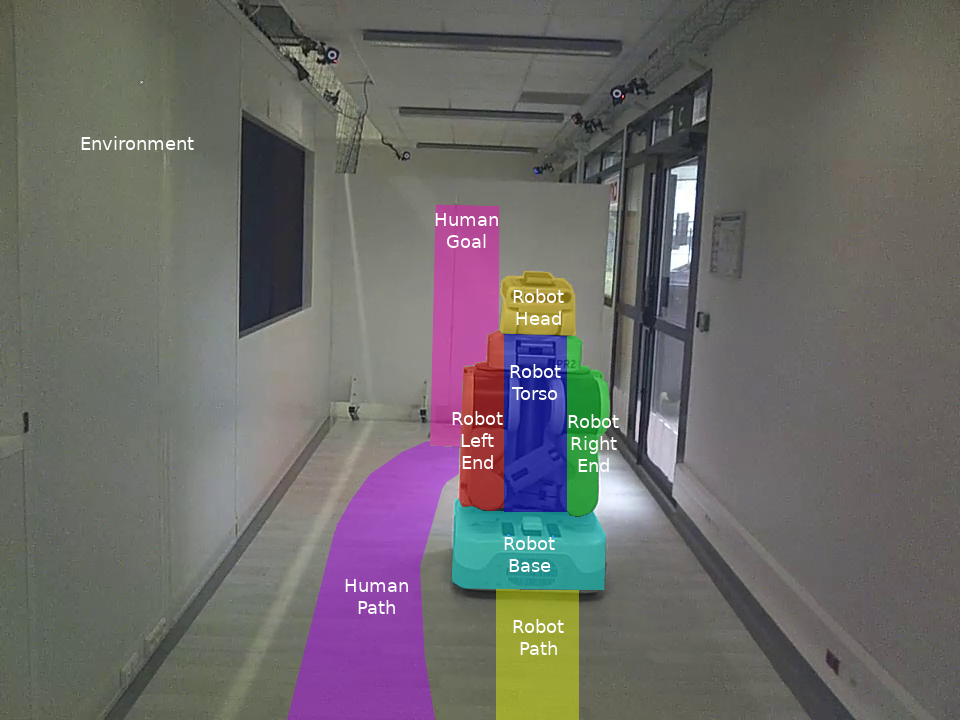
\includegraphics[scale=0.4]{figures/chapter2/pr2_aois_2.png}
\caption{The areas of interest defined to analyze the participants oculometric data.}
\label{fig:aois}
\end{figure}

\item \textit{Interview}:
The first question was a control question, ensuring that the participants saw differences between each blocks. After the second question, the interviewer revealed that the robot behavior was indeed different between each block, then proceeded to the rest of the interview. The participants answers were analyzed by excerpting verbatim (keywords or general ideas) from each question and computing their frequencies.

\item \textit{Dependent variables}:
Therefore, the dependent variables were the participant scores at the three questionnaires: PeRDITA, Situation Awareness and AttrakDiff, in addition to the number and duration of their gaze fixation during the crossing.
Prior to the experiment, the participants were asked to fill a questionnaire inquiring their age, gender, education level, profession, native language, an open question about past experience with robots and a 7 points Likert scale assessing their overall opinion about robotics.
\end{enumerate}

\subsection{Results}
\subsection{Quantitative results}
During the crossing almost all participants (95\%) went to their left (thus, letting the robot go to their right) because the experimental setup led them to do so as the interview revealed. The robot also planned that the optimal path (given the constraints described above) was to go to the right of the human. Participants who went to their right stated they were "testing" the robot, thus not respecting the given goal (which was to go to the marked goal and not to test the robot). These trials have been removed from the data.

\subsubsection{Pertinence of Robot Decision In joinT Action}
The mean scores of the three dimensions of the PeRDITA questionnaire were significantly higher with an alternating head behavior than with a continuous one. The quality of interaction was higher with an alternating head behavior (\textit{M} = 5.31, \textit{SD} = 0.97), than with a continuous head behavior (\textit{M} = 5.03, \textit{SD} = 1.17), \textit{F}(1,26) = 4.41, \textit{p} < .05, $\eta_{p}^{2}$ = .15. The perceived robot competence was higher with an alternating head behavior (\textit{M} = 5.12, \textit{SD} = 1.14), than with a continuous one (\textit{M} = 4.73, \textit{SD} = 1.14), \textit{F}(1,26) = 9.15, \textit{p} < .01, $\eta_{p}^{2}$ = .26. The quality of collaboration was higher with an alternating head behavior  (\textit{M} = 5.06, \textit{SD} = 1.04), than with a continuous one (\textit{M} = 4.73, \textit{SD} = 1.14), \textit{F}(1,26) = 6.07, \textit{p} < .05, $\eta_{p}^{2}$ = .19.

There was not any significant effect of TTC on the quality of interaction (\textit{F}(1,26) = 1.65, \textit{p} = .21.), on the perceived robot competence (\textit{F}(1,26) = 0.04, \textit{p} = .84), and on the quality of collaboration neither (\textit{F}(1,26) = 0.43, \textit{p} = .52). No interaction between TTC and head behaviors reached significance.

\subsubsection{Attrakdiff}
The mean score of the hedonic qualities dimension was higher with an alternating head behavior (\textit{M} = 5.06, \textit{SD} = 0.87), than with a continuous one (\textit{M} = 4.93, \textit{SD} = 0,82), \textit{F}(1,26) = 4.13, \textit{p} < .05, $\eta_{p}^{2}$ = .14. There was no significant differences regarding the scores of the pragmatic qualities (\textit{F}(1,26) = 0.34, \textit{p} = .57) and attractiveness (\textit{F}(1,26) = 0.14, \textit{p} = .71) dimensions. 

There was not any significant effect of TTC on hedonic qualities (\textit{F}(1,26) = 3.25, \textit{p} = .08), on pragmatic qualities (\textit{F}(1,26) = 2.97, \textit{p} = .10), and on attractiveness neither (\textit{F}(1,26) = 0.37, \textit{p} = .55). No interaction between TTC and head behaviors reached significance.

\subsubsection{Situation awareness}
The mean score of global situation awareness was significantly higher with an alternating head behavior (\textit{M} = 4.64, \textit{SD} = 0.98), than with a continuous one (\textit{M} = 4.33, \textit{SD} = 1.12), \textit{F}(1,26) = 7.77, \textit{p} < .01, $\eta_{p}^{2}$ = .23.

The mean scores of all the three dimensions of situation awareness were higher with an alternating head behavior than with a continuous one. Perception was significantly higher with an alternating head behavior (\textit{M} = 4.60, \textit{SD} = 1.08), than with a continuous one (\textit{M} = 4.15, SD = 1.29), \textit{F}(1,26) = 8.20, \textit{p} < .01, $\eta_{p}^{2}$ = .24. Comprehension was higher with an alternating head behavior (\textit{M} = 4.64, \textit{SD} = 1.05), than on a continuous one (\textit{M} = 4.36, \textit{SD} = 1.14), \textit{F}(1,26) = 5.99, \textit{p} < .05, $\eta_{p}^{2}$ = .19. Projection was higher (strong tendency) with an alternating head behavior (\textit{M} = 4.67, \textit{SD} = 0.96), than on a continuous one (\textit{M} = 4.47, \textit{SD} = 1.16), \textit{F}(1,26) = 3.52, \textit{p} = .07, $\eta_{p}^{2}$ = .12.

There was not any significant effect of the TTC on global situation awareness (\textit{F}(1,26) = 1.70, \textit{p} = .20), on the perception dimension (\textit{F}(1,26) = 0.72, p = .41), and on the comprehension dimension (\textit{F}(1,26) = 0.60, \textit{p} = .45). However, the mean score of the projection dimension was higher (strong tendency) with a high TTC (\textit{M} = 4.69, \textit{SD} = 0.98), than with a low TTC (\textit{M} = 4.44, \textit{SD} = 1.13), \textit{F}(1,26) = 4.03, \textit{p} = .06, $\eta_{p}^{2}$ = .13. No interaction between TTC and head behaviors reached significance.

\subsubsection{Gaze}
\begin{itemize}
\item  \textit{Robot vs. Environment}

The mean number of eye fixations was significantly higher on the robot (\textit{M} = 2.23, \textit{SD} = 0.98) than on the environment (\textit{M} = 1.17, \textit{SD} = 0.90), \textit{F}(1,21) = 17.82, \textit{p} < .001, $\eta_{p}^{2}$ = .46.
The mean number of eye fixations was higher (strong tendency) with a high TTC (\textit{M} = 1.76, \textit{SD} =  1.04) than with a low TTC (\textit{M} = 1.65, \textit{SD} = 1.11), \textit{F}(1,21) = 3.86, \textit{p} = .06, $\eta_{p}^{2}$ = .16, regardless of the AOIs. There was not any significant effect of the robot head behavior on the mean number of eye fixations, \textit{F}(1,21) = 0.90, \textit{p} = .35. No interaction between the three factors reached significance.

The mean average duration of eye fixations was significantly higher on the robot (\textit{M} = 351, \textit{SD} =  172) than on the environment (\textit{M} = 260, \textit{SD} = 123), \textit{F}(1,18) = 6.95, \textit{p} < .05, $\eta_{p}^{2}$ = .28. There was not any other significant effects or interactions regarding the average duration of eye fixations.

\item \textit{Robot AOIs}

As shown in Table~\ref{table:eye_fixation_ttc_head}, the head was the part of the robot that was the most fixated by the participants (\textit{M} = 6.13 ; \textit{SD} = 0.59), \textit{F}(4,84) = 39.10, \textit{p} < .001, $\eta_{p}^{2}$ = .65. The number of fixations on other parts were \textit{M} = 1.28 (\textit{SD} = 0.31) for the base, \textit{M} = 1.16 (\textit{SD} = 0.23) for the torso, \textit{M} = 0.95 (\textit{SD} = 0.19) for the right end, and \textit{M} = 1.64 (\textit{SD} = 0.37) for the left end. 

\begin{table}[!htbp]
   \caption{\label{table:eye_fixation_ttc_head} Mean number of eye fixations made by participants in each area of interest (AoI) of the robot in each experimental condition (TTC x robot head behavior) in main experiment. Standard deviations are shown in parentheses.}
    \begin{tabular}{lcccc}
    \hline
    \multirow{2}{*}{\textbf{Robot AoI}} & \multicolumn{2}{c}{\textbf{Low TTC}} & \multicolumn{2}{c}{\textbf{High TTC}} \\
    \cline{2-5} 
               & \textbf{Continuous}  & \textbf{Alternating}  & \textbf{Continuous}  & \textbf{Alternating}   \\
    \hline
    Head       & 5.64 (3.42)  & 5.50 (2.78)  & 5.93 (2.90)  & 7.45 (3.80)   \\
    Torso      & 1.39 (1.39)  & 1.14 (1.49)  & 1.39 (1.65)  & 0.73 (0.96)   \\
    Left end   & 0.95 (1.20)  & 1.07 (1.11)  & 1.00 (1.15)  & 0.77 (1.14)   \\
    Right end  & 1.82 (1.92)  & 1.55 (1.71)  & 1.55 (1.94)  & 1.64 (2.27)   \\
    Base       & 1.36 (2.07)  & 1.23 (1.53)  & 1.45 (1.65)  & 1.07 (1.27)   \\
    \hline
\end{tabular}
\end{table}

There was a significant interaction between the AOI type and the type of TTC, \textit{F}(4,84) = 5.72, \textit{p} < .001, $\eta_{p}^{2}$ = .21. The robot head was more fixated when the TTC was high (\textit{M} = 6.69, \textit{SD} = 3.43) than when it was low (\textit{M} = 5.57, \textit{SD} = 3.08). There was an interaction (strong tendency) between the AOI type and head behaviors, \textit{F}(4,84) = 2.34, \textit{p} = .06, $\eta_{p}^{2}$ = .10. The robot head was more fixated, when the robot head was alternating  (\textit{M} = 6.48, \textit{SD} = 3.43) than when it was continuous (\textit{M} = 5.78, \textit{SD} = 3.14).

In addition, there was a double interaction (strong tendency) between the AOI type, head behaviors and the type of TTC, \textit{F}(4,84) = 2.41, \textit{p} = .06, $\eta_{p}^{2}$ = .10. Table~\ref{table:eye_fixation_ttc_head} shows that the robot head was more fixated when the robot head was alternating only with a high TTC.

There was not any significant effect of the robot head behaviors on the mean number of eye fixations, \textit{F}(1,21) = 0.13, \textit{p} = .73. There was not any significant effect of the TTC type on the mean number of eye fixations, \textit{F}(1,21) = 1.82, \textit{p} = .19. The interaction between the TTC and the head behaviors, \textit{F}(1,21) = 0.74, \textit{p} = .40, did not reach significance.

The ANOVA for the mean duration of eye fixations was not possible due to an absence of data in some experimental conditions.
\end{itemize}

\subsection{Qualitative results}
All the participants saw differences between blocks, 19 of them saw head behavior differences and 10 of them saw trajectory differences. When the participant talked about the alternated head behavior, positive adjectives were employed ("reassuring", "sympathetic", "interactive"), when they talked about the continuous head behavior, negative adjectives were employed ("unsettling").

After the experimenter revealed that the robot behavior was different in each block, the participants preferred when the robot was "moving its head" (12 participants). Five participants also preferred when the robot changes its direction long before they cross. Participants did not appreciate when the robot kept a "fixed head" because they thought the robot was not aware of them (8 participants), when the robot was "hesitating" (4 participants) and when it came "too close" (4 participants).

Fourteen participants found the robot was the most competent in the condition with the alternated head behavior and high TTC, because the robot became aware of them when looking at them (10 participants), because the robot changed its direction sooner (4 participants), because it was trying to avoid them (4 participants) or because it was not coming too close (3 participants).

The participants found the robot more acceptable when it made a "visual contact" (4 participants) and when it changed its trajectory early (3 participants). They found the robot less acceptable when the robot came too close (6 participants), when hesitating (3 participants), when not making visual contact (2 participants).


\subsection{Discussion}
This study aimed at exploring how taking into account the human model and planning for both human and robot during navigation allows to easily design behavior enhancing the usability of the robot. More precisely, navigation coplanning allows to easily implement coordination smoothers and increase mutual manifestness, we thus hypothesized that these changes should lead to a significant impact on robot usability in the intricate scenario of narrow corridor crossing.

Human gaze analysis showed that head of the robot was fixed many times and even more when the robot showed its chosen corridor side early in the navigation (with a high TTC). Moreover, subjective results revealed that moving the head of the robot in an alternating pattern (pointing towards its path while sometimes pointing at the human head) improved the perception of the quality of interaction, the perceived robot competence, and the quality of collaboration. This alternative head behavior also increases the situation awareness score. This strongly support previous results on using the robot head during human robot navigation scenarios \cite{khambhaita_head-body_2016}, \cite{may_show_2015}.

However, the satisfaction seems to have been slightly improved (on hedonic quality) when the robot presented the alternating gaze behavior rather than the continuous one. This result is only a tendency, but in the interview, the participants identified as positive when the robot moved its head to glance at them and changed its trajectory. They also identified as negative when the robot was too close or did not look at them. We think these discrepancies between the AttrakDiff results and the interview are caused by our poor questionnaire choice. Indeed, the AttrakDiff questionnaire aims at measuring the satisfaction produced by a final product (\textit{e.g.} cellphones) and the willingness of a user to buy this product, but not the satisfaction of a user when dynamically interacting with a robot in a navigation scenario. Yet, as no other questionnaire to our knowledge proposed to measure user satisfaction during human robot interaction, we chose the AttrakDiff.

Results show that using the HATEB navigation co-planner with a high time-to-collision weight constraint cost and low threshold, alongside an head behavior signaling future robot trajectory and the human awareness during a crossing in a constrained space allows the human to have a better situation awareness and to perceive the robot as acting more pertinently and being more competent. This finding support the result from Lu et al. \cite{lu_towards_2013}, where the navigation efficiency is increased when the robot looks at the human and shows a "social" navigation behavior.

We speculate that both the high TTC and alternating gaze of the robot are needed to improve the interaction and that no simple effect are significant for multiple reasons. First, with only the robot choosing a corridor side early in the crossing (high TTC condition) without showing the human awareness (continuous head condition), it may not be obvious to the human that the trajectory change is due to their presence. Conversely, when the robot signals its awareness of the human (here by pointing its head towards them) but without taking any action to ease the interaction (low TTC condition), the human stays in a situation where they don't know what the robot will do next. Finally, by both making the robot show its human awareness and change its own trajectory to facilitate the interaction (coordination smoother), it becomes clear the that robot is proposing a co-navigation solution where both agents are avoiding each other.

Finally, oculometry results indicate that when the head is recognized as an information provider (in the alternating head condition), information are most likely to be sought in the robot head motion. The head is also looked longer when the robot alternately looks at the human. We can also note that people tend to think PR2 is getting data through its head, probably because of the visible cameras on it, even when it is not the case (like in our experiment).

\improvement{Ajouter limites et future works de l'étude ? Ou le mettre dans la section conclusion ?}

\section{Extending HATEB}
Having shown that providing co-navigation solution using HATEB can effectively be used to enhance the efficiency of the interaction, we will present in this section the different extensions made to HATEB.

\subsection{Adapting HATEB to other robots}
Khambhaita et al. \cite{khambhaita_head-body_2016} successfully used HATEB on a PR2 robot, both in simulation and on the real platform. As the approach is general, we implemented it on other robots.

\subsubsection{Humanoid Robot}
Humanoid robots are characterized by their bipedal navigation, tremendously increasing the complexity of simple navigation with regards to wheeled robots. However, legged robots present a large advantage for social and human robot interaction as human infrastructure are often thought for being navigated with legs rather than with wheels. Thus, we tried to implement our approach to a humanoid robot.

To do so, we partnered with the Gepetto team at LAAS-CNRS specialized in humanoid systems motion. Thanks to their modular software architecture presented in \cite{stasse_modular_architecture_2008}, only minor changes had to be done to HATEB to integrate with their other components.

One of their component \cite{naveau_reactive_walking_2017} takes as parameter a (simplified) robot kinematic model and is able, in real-time and at typical joint position control frequencies (around 200~Hz), to give position command to all the robot joints in order for the center of mass of the robot to respect a speed command given as input. To do so, the component needs to generate footstep placements and to compute robot joint positions ensuring the equilibrium and the respect of the kinodynamic constraints (between two successive poses) of the robot. However, this component as no ROS interface whereas HATEB is heavily built for ROS use. Thus, we made a bridge transferring the speed commands output by HATEB to the Gepetto architecture and transferring back the joint position commands.

This has only be run virtually, and for simplicity, no simulator was used. Instead, we assumed the joint position command to be immediately and perfectly executed. Such an assumption has been made possible because of the effectiveness of the Gepetto architecture, having a tested precise model of the robot, ensures that the kinodynamic constraints will be respected, and consequently gives a correct robot behavior.

We tested this approach on a virtual HRP2 robot, with a virtual human. \unsure{What result do I have from that?} 

\subsubsection{Pepper robot for close human robot motions}
The European project MuMMER aimed at deploying a Pepper robot in a shopping mall in Finland to entertain and guide customers. \improvement[inline]{ref} The project united seven different stakeholders bringing their knowledge to the project. The LAAS-CNRS goal was to make the guide task. However, in order to serve the most customers possible and to cope with large navigation issues of the Pepper platform, we choose not to go with the customer all the way to the asked shop, but instead, as the mall employees usually do, give directions to the customer to help them find the requested shop.
However, giving only verbal instructions concerning the route is not sufficient, we chose to make the robot point the shop, if it is visible from the current position, or point its direction and the first visible element of the route otherwise.

Although, the surroundings of the robot home place (the place in the mall where the robot is located, and thus, where the interaction takes place) contains some obstacles such as barriers, structure poles and advertisement posters. Thus, the object the robot has to point to the human might not be visible from their current position. We thus endowed the robot with the ability to compute the optimal position for the human and the robot for it to point at a landmark. This computation details can be found in \cite{waldhart_reasoning_shared_2019}. Once the robot has computed these optimal positions, it needs to move to its one while ensuring the human can move to theirs. Moreover, the customers might be hesitant to approach the robot to start an interaction, thus, the robot is also able to approach a nearby human to ask them if they need its help. However, it has to consider that the human might also move towards the robot to encounter it.

To tackle both of these issues, we decided to use HATEB. We made a higher level component proposing three services: rotate, navigate to and approach. While the rotate service is only made for in place rotation of the robot in order to reorient itself for repositioning or to look or point at something, the other two uses the HATEB planner described earlier. The navigate to service expects a robot goal pose and optionally a human identifier and a human goal (which is shown by the robot before starting the navigation). The HATEB planner is then called with empirically tuned weights to make the robot navigate to its goal position while, if provided, ensuring the human can reach theirs. The approach service expects a human identifier and a distance, and use the HATEB planner with different weights (e.g. with the visibility constraint described in \ref{sect:chapter2_visibility_constraint} activated) with a goal at the specified distance in front of the human. The human goal is predicted from their current pose and velocity some seconds in the future, and updated at each control loop with their new sensed pose and speed.

While this scheme worked well for the approach, with the robot presenting an efficient approach trajectory reacting the human motion, it performed very poorly for the navigation part. Indeed, the robot navigation was erratic and made too long trajectories even between close start and goal points. We identified two causes to this over conservative behavior:

\begin{itemize}
\item First, the HATEB algorithm did not support holonomic motion. Although this was not a problem for long distance scenarios, it made the robot having to maneuver to achieve small displacements.

\item Then, by planning these short trajectories so close to the human, the optimizer does not have a lot of latitude to play with, and the search space is very noisy and chaotic.
\end{itemize}

It has thus been decided in the project to not use the HATEB approach, but simply an holonomic timed elastic band enriched with social constraints linked to the nearby humans (\textit{i.e.} only optimizing the robot trajectory and not the human one).

This allowed to point out some of the limitations of the HATEB approach, it performs poorly for small, intricate displacements. This led to the creation of HATEB2 \cite{teja_hateb2_2020}, which is able to switch online between the HATEB planner, the TEB planner with social constraints or a velocity obstacle planner.

\unsure{HATEB 3D ?}

\subsection{Using the estimated time to goal to measure the execution of the planned trajectory}

Another benefit of the HATEB approach is that it does not only compute speed command to follow a global plan while avoiding obstacles like other classic local planner, but also returns a complete short term trajectory for both the robot and the human. Moreover, as the trajectories contains the expected duration between each pose, simply by summing them, we can have an estimate of the time remaining to execute the local trajectories. Besides, we also compute the estimated time remaining for the global trajectories after the local ones by dividing the computed speed at the last local trajectory pose by its length. By summing these two estimated remaining times, we can have a estimation of the remaining navigation time (the time to goals) for all the considered agents.

By monitoring the evolution of these times, we can estimate a quality of the ongoing navigation. Indeed, the local trajectories are computed at at a position control rate and so are the time to goals. Intuitively, if the computed time to goals are decreasing at the same rate as the real time duration (\textit{e.g.} the estimation for the robot goes from 12 seconds to 11 seconds while one second has elapsed) the execution of the trajectories are going according to plan. Instead, if the computed time to goals are decreasing slower than the real time duration, staying equals or even increasing, the execution does not go as smoothly as the plan was.

We formalized it as follows: 
\begin{equation}
s_i(t) = \frac{ttg_i(t) - ttg_i(t - x)}{x}
\end{equation}
with $s_i(t)$ is the time to goal variation for the trajectory $i$ (either the robot or one of the considered human) at time $t$, and $x$ is the time window size parameter, specifying how old are the previous time to goal value we are comparing the current one with.
With this definition we have:
\begin{itemize}
\item $s(t) \approx 1$: the execution goes according to plan,
\item $s(t) > 1$: the execution outperforms the plan,
\item $0 < s(t) < 1$: the execution goes slower than the plan, but progress towards the goal is still being made,
\item and $s(t) < 0$: the goal is getting further.
\end{itemize}

This value can then be fed back to a supervision system which can change the navigation parameters or abort it to make a repair strategy if, combined with other task monitored values, it judges the navigation action is endangering the higher level task.

\unsure{images ?}

\improvement{Dire que même si ça permet une certaine évaluation ça ne dit pas le problème. Obstacle imprévu par le robot ? Human qui change d'avis ? Humain qui ne veut pas coopérer ? Mauvais modèle de l'humain ?}



\subsection{Adding constraints}
\unsure{Is this subsection useful ?}


\subsubsection{The visibility constraint}
\label{sect:chapter2_visibility_constraint}

\unsure{ttc plus ?}


\section{Conclusion}
\todo{Limitations: Mouvement trop courts et proches de l'humain (Mummer), nécessite d'avoir un bon modèle de l'humain (robot qui suit l'humain en pensant qu'il va accelerer), trouve le plan optimal comme si l'humain allait être au courant: c'est bien ça permet de s'assurer qu'il en existe au moins une trajectoire pour l'humain, mais ce n'est peut-être pas celle qu'il va choisir et on risque de se mettre dans un deadlock (en pensant qu'il va choisir une trajectoire mais en fait il en fait une autre).}

In this chapter, we presented a robot navigation planner HATEB, which not only computes an optimal local trajectory for the robot but also for the surrounding humans. This approach has been shown to be able to solve complex navigation tasks where both agents must take cooperate to reach their respective goals. Moreover, we proved via an user study that it allows to implement effective coordination smoothers to increase the robot mutual manifestness and facilitate the whole interaction.
Besides, the versatility of this approach has been presented via its implementation on three different robots: PR2, HRP2 and Pepper.
Finally, we used an other benefit of this scheme which is to compute precise local trajectory at position control loop rate to estimate the remaining time to reach the navigation goal. By processing this data and monitoring it over the course of interaction, quality of the ongoing navigation and interaction can be deduced and returned to a higher level supervision component.

We are particularly interested in these coordination smoothers, which can be seen as non verbal communication of the robot intents and of the shared plan. Planning for these coordination smoothers can only be done if we plan for both the robot and the human. However, due to the continuous and short duration nature inherent to navigation tasks, exploring the planning of such communication can be tedious. We thus propose to move from navigation problems to focus on human robot symbolic task planning.


\ifdefined\included
\else
\bibliographystyle{acm}
\bibliography{These}
\end{document}
\fi

\ifdefined\included
\else
\documentclass[a4paper,11pt,twoside]{StyleThese}
\usepackage{amsmath,amssymb, amsthm}             % AMS Math
\usepackage[T1]{fontenc}
\usepackage[utf8x]{inputenc}
\usepackage{babel}
\usepackage{datetime}

\usepackage{silence}

\WarningFilter{minitoc(hints)}{W0023}
\WarningFilter{minitoc(hints)}{W0028}
\WarningFilter{minitoc(hints)}{W0030}

\usepackage{lmodern}
\usepackage{tabularx}
%\usepackage{tabular}
\usepackage{multirow}
\usepackage{xspace}

\usepackage{hhline}
\usepackage[left=1.5in,right=1.3in,top=1.1in,bottom=1.1in,includefoot,includehead,headheight=13.6pt]{geometry}
\renewcommand{\baselinestretch}{1.05}

% Table of contents for each chapter

\usepackage[nottoc, notlof, notlot]{tocbibind}
\usepackage{minitoc}
\setcounter{minitocdepth}{2}
\mtcindent=15pt
% Use \minitoc where to put a table of contents

\usepackage{aecompl}

% Glossary / list of abbreviations

\usepackage[intoc]{nomencl}
\iftoggle{ThesisInEnglish}{%
\renewcommand{\nomname}{Glossary}
}{ %
\renewcommand{\nomname}{Liste des Abréviations}
}

\usepackage{etoolbox}
\renewcommand\nomgroup[1]{%
  \item[\bfseries
  \ifstrequal{#1}{A}{Number Sets}{%
  \ifstrequal{#1}{G}{Agents Beliefs and Action Models}{%
  \ifstrequal{#1}{N}{Navigation}{%
  \ifstrequal{#1}{O}{Ontology}{%
  \ifstrequal{#1}{R}{Referring Expression Generation}{%
  \ifstrequal{#1}{Z}{Controllable and Uncontrollable Agents Task Planning}{}}}}}}%
]}

\makenomenclature



% My pdf code

\usepackage{ifpdf}

\ifpdf
  \usepackage[pdftex]{graphicx}
  \DeclareGraphicsExtensions{.jpg}
  \usepackage[pagebackref,hyperindex=true]{hyperref}
  \usepackage{tikz}
  \usetikzlibrary{arrows,shapes,calc}
\else
  \usepackage{graphicx}
  \DeclareGraphicsExtensions{.ps,.eps}
  \usepackage[dvipdfm,pagebackref,hyperindex=true]{hyperref}
\fi

\graphicspath{{.}{images/}}

%% nicer backref links. NOTE: The flag ThesisInEnglish is used to define the
% language in the back references. Read more about it in These.tex

\iftoggle{ThesisInEnglish}{%
\renewcommand*{\backref}[1]{}
\renewcommand*{\backrefalt}[4]{%
\ifcase #1 %
(Not cited.)%
\or
(Cited in page~#2.)%
\else
(Cited in pages~#2.)%
\fi}
\renewcommand*{\backrefsep}{, }
\renewcommand*{\backreftwosep}{ and~}
\renewcommand*{\backreflastsep}{ and~}
}{%
\renewcommand*{\backref}[1]{}
\renewcommand*{\backrefalt}[4]{%
\ifcase #1 %
(Non cité.)%
\or
(Cité en page~#2.)%
\else
(Cité en pages~#2.)%
\fi}
\renewcommand*{\backrefsep}{, }
\renewcommand*{\backreftwosep}{ et~}
\renewcommand*{\backreflastsep}{ et~}
}

% Links in pdf
\usepackage{color}
\definecolor{linkcol}{rgb}{0,0,0.4} 
\definecolor{citecol}{rgb}{0.5,0,0} 
\definecolor{linkcol}{rgb}{0,0,0} 
\definecolor{citecol}{rgb}{0,0,0}
% Change this to change the informations included in the pdf file

\hypersetup
{
bookmarksopen=true,
pdftitle="Planning For Both Robot and Human: Anticipating and Accompanying Human Decisions",
pdfauthor="Guilhem BUISAN", %auteur du document
pdfsubject="Thèse", %sujet du document
%pdftoolbar=false, %barre d'outils non visible
pdfmenubar=true, %barre de menu visible
pdfhighlight=/O, %effet d'un clic sur un lien hypertexte
colorlinks=true, %couleurs sur les liens hypertextes
pdfpagemode=None, %aucun mode de page
pdfpagelayout=SinglePage, %ouverture en simple page
pdffitwindow=true, %pages ouvertes entierement dans toute la fenetre
linkcolor=linkcol, %couleur des liens hypertextes internes
citecolor=citecol, %couleur des liens pour les citations
urlcolor=linkcol %couleur des liens pour les url
}

% definitions.
% -------------------

\setcounter{secnumdepth}{3}
\setcounter{tocdepth}{2}

% Some useful commands and shortcut for maths:  partial derivative and stuff

\newcommand{\pd}[2]{\frac{\partial #1}{\partial #2}}
\def\abs{\operatorname{abs}}
\def\argmax{\operatornamewithlimits{arg\,max}}
\def\argmin{\operatornamewithlimits{arg\,min}}
\def\diag{\operatorname{Diag}}
\newcommand{\eqRef}[1]{(\ref{#1})}

\usepackage{rotating}                    % Sideways of figures & tables
%\usepackage{bibunits}
%\usepackage[sectionbib]{chapterbib}          % Cross-reference package (Natural BiB)
%\usepackage{natbib}                  % Put References at the end of each chapter
                                         % Do not put 'sectionbib' option here.
                                         % Sectionbib option in 'natbib' will do.
\usepackage{fancyhdr}                    % Fancy Header and Footer

% \usepackage{txfonts}                     % Public Times New Roman text & math font
  
%%% Fancy Header %%%%%%%%%%%%%%%%%%%%%%%%%%%%%%%%%%%%%%%%%%%%%%%%%%%%%%%%%%%%%%%%%%
% Fancy Header Style Options

\pagestyle{fancy}                       % Sets fancy header and footer
\fancyfoot{}                            % Delete current footer settings

%\renewcommand{\chaptermark}[1]{         % Lower Case Chapter marker style
%  \markboth{\chaptername\ \thechapter.\ #1}}{}} %

%\renewcommand{\sectionmark}[1]{         % Lower case Section marker style
%  \markright{\thesection.\ #1}}         %

\fancyhead[LE,RO]{\bfseries\thepage}    % Page number (boldface) in left on even
% pages and right on odd pages
\fancyhead[RE]{\bfseries\nouppercase{\leftmark}}      % Chapter in the right on even pages
\fancyhead[LO]{\bfseries\nouppercase{\rightmark}}     % Section in the left on odd pages

\let\headruleORIG\headrule
\renewcommand{\headrule}{\color{black} \headruleORIG}
\renewcommand{\headrulewidth}{1.0pt}
\usepackage{colortbl}
\arrayrulecolor{black}

\fancypagestyle{plain}{
  \fancyhead{}
  \fancyfoot{}
  \renewcommand{\headrulewidth}{0pt}
}

%\usepackage{MyAlgorithm}
%\usepackage[noend]{MyAlgorithmic}
\usepackage{algorithm}
\usepackage[noend]{algpseudocode}
\usepackage{comment}
\usepackage[ED=EDSYS-Robo, Ets=INSA]{tlsflyleaf}
%%% Clear Header %%%%%%%%%%%%%%%%%%%%%%%%%%%%%%%%%%%%%%%%%%%%%%%%%%%%%%%%%%%%%%%%%%
% Clear Header Style on the Last Empty Odd pages
\makeatletter

\def\cleardoublepage{\clearpage\if@twoside \ifodd\c@page\else%
  \hbox{}%
  \thispagestyle{empty}%              % Empty header styles
  \newpage%
  \if@twocolumn\hbox{}\newpage\fi\fi\fi}

\makeatother
 
%%%%%%%%%%%%%%%%%%%%%%%%%%%%%%%%%%%%%%%%%%%%%%%%%%%%%%%%%%%%%%%%%%%%%%%%%%%%%%% 
% Prints your review date and 'Draft Version' (From Josullvn, CS, CMU)
\newcommand{\reviewtimetoday}[2]{\special{!userdict begin
    /bop-hook{gsave 20 710 translate 45 rotate 0.8 setgray
      /Times-Roman findfont 12 scalefont setfont 0 0   moveto (#1) show
      0 -12 moveto (#2) show grestore}def end}}
% You can turn on or off this option.
% \reviewtimetoday{\today}{Draft Version}
%%%%%%%%%%%%%%%%%%%%%%%%%%%%%%%%%%%%%%%%%%%%%%%%%%%%%%%%%%%%%%%%%%%%%%%%%%%%%%% 

\newenvironment{maxime}[1]
{
\vspace*{0cm}
\hfill
\begin{minipage}{0.5\textwidth}%
%\rule[0.5ex]{\textwidth}{0.1mm}\\%
\hrulefill $\:$ {\bf #1}\\
%\vspace*{-0.25cm}
\it 
}%
{%

\hrulefill
\vspace*{0.5cm}%
\end{minipage}
}

\let\minitocORIG\minitoc
\renewcommand{\minitoc}{\minitocORIG \vspace{1.5em}}

\usepackage{multirow}
%\usepackage{slashbox}

\newenvironment{bulletList}%
{ \begin{list}%
	{$\bullet$}%
	{\setlength{\labelwidth}{25pt}%
	 \setlength{\leftmargin}{30pt}%
	 \setlength{\itemsep}{\parsep}}}%
{ \end{list} }

\theoremstyle{definition}
\newtheorem{definition}{Definition}
\renewcommand{\epsilon}{\varepsilon}

% centered page environment

\newenvironment{vcenterpage}
{\newpage\vspace*{\fill}\thispagestyle{empty}\renewcommand{\headrulewidth}{0pt}}
{\vspace*{\fill}}

\usepackage{tablefootnote}

\theoremstyle{plain}
\newtheorem{constraint}{Constraint}[section]

\algnewcommand\algorithmicforeach{\textbf{for each}}
\algnewcommand\algorithmicin{\textbf{in}}
\algdef{S}[FOR]{ForEach}[2]{\algorithmicforeach\ #1\ \algorithmicin\ #2\ \algorithmicdo}

\usepackage{listings}
\lstdefinestyle{customPlan}{
  language=C,
  commentstyle=\itshape\color{green!25!black},
}
\usepackage{pdfpages}

\sloppy
\begin{document}
\setcounter{chapter}{2} %% Numéro du chapitre précédent ;)
\dominitoc
\faketableofcontents
\fi

\chapter{Evaluating communication needs at task planning level}
\minitoc

\section{Introduction}


\section{Related Work}
\subsection{Referring Expression Generation}

Il faut utilizer au moins une citation (exemple: \cite{goossens93}) pour bien
compiler le document. Regardez le document These.bib pour les details de
comment organizer la bibliographie.

\subsection{Task Planning with Communication Actions}

Pour ajouter un symbole à la liste des abréviations il faut utiliser
\verb|\nomenclature{<symbole>}{<description>}|. Par exemple, je peux ajouter
$\beta$\nomenclature{$\beta$}{La deuxième lettre de l'alphabet grec} et
$\alpha$\nomenclature{$\alpha$}{La première lettre de l'alphabet grec} comme
symboles dans ce document.

\section{Ontology based Referring Expression Generation}

\section{Planning Communication Actions Using Referring Expression Generation}

\ifdefined\included
\else
\bibliographystyle{acm}
\bibliography{These}
\end{document}
\fi

\ifdefined\included
\else
\documentclass[a4paper,11pt,twoside]{StyleThese}
\usepackage{amsmath,amssymb, amsthm}             % AMS Math
\usepackage[T1]{fontenc}
\usepackage[utf8x]{inputenc}
\usepackage{babel}
\usepackage{datetime}

\usepackage{silence}

\WarningFilter{minitoc(hints)}{W0023}
\WarningFilter{minitoc(hints)}{W0028}
\WarningFilter{minitoc(hints)}{W0030}

\usepackage{lmodern}
\usepackage{tabularx}
%\usepackage{tabular}
\usepackage{multirow}
\usepackage{xspace}

\usepackage{hhline}
\usepackage[left=1.5in,right=1.3in,top=1.1in,bottom=1.1in,includefoot,includehead,headheight=13.6pt]{geometry}
\renewcommand{\baselinestretch}{1.05}

% Table of contents for each chapter

\usepackage[nottoc, notlof, notlot]{tocbibind}
\usepackage{minitoc}
\setcounter{minitocdepth}{2}
\mtcindent=15pt
% Use \minitoc where to put a table of contents

\usepackage{aecompl}

% Glossary / list of abbreviations

\usepackage[intoc]{nomencl}
\iftoggle{ThesisInEnglish}{%
\renewcommand{\nomname}{Glossary}
}{ %
\renewcommand{\nomname}{Liste des Abréviations}
}

\usepackage{etoolbox}
\renewcommand\nomgroup[1]{%
  \item[\bfseries
  \ifstrequal{#1}{A}{Number Sets}{%
  \ifstrequal{#1}{G}{Agents Beliefs and Action Models}{%
  \ifstrequal{#1}{N}{Navigation}{%
  \ifstrequal{#1}{O}{Ontology}{%
  \ifstrequal{#1}{R}{Referring Expression Generation}{%
  \ifstrequal{#1}{Z}{Controllable and Uncontrollable Agents Task Planning}{}}}}}}%
]}

\makenomenclature



% My pdf code

\usepackage{ifpdf}

\ifpdf
  \usepackage[pdftex]{graphicx}
  \DeclareGraphicsExtensions{.jpg}
  \usepackage[pagebackref,hyperindex=true]{hyperref}
  \usepackage{tikz}
  \usetikzlibrary{arrows,shapes,calc}
\else
  \usepackage{graphicx}
  \DeclareGraphicsExtensions{.ps,.eps}
  \usepackage[dvipdfm,pagebackref,hyperindex=true]{hyperref}
\fi

\graphicspath{{.}{images/}}

%% nicer backref links. NOTE: The flag ThesisInEnglish is used to define the
% language in the back references. Read more about it in These.tex

\iftoggle{ThesisInEnglish}{%
\renewcommand*{\backref}[1]{}
\renewcommand*{\backrefalt}[4]{%
\ifcase #1 %
(Not cited.)%
\or
(Cited in page~#2.)%
\else
(Cited in pages~#2.)%
\fi}
\renewcommand*{\backrefsep}{, }
\renewcommand*{\backreftwosep}{ and~}
\renewcommand*{\backreflastsep}{ and~}
}{%
\renewcommand*{\backref}[1]{}
\renewcommand*{\backrefalt}[4]{%
\ifcase #1 %
(Non cité.)%
\or
(Cité en page~#2.)%
\else
(Cité en pages~#2.)%
\fi}
\renewcommand*{\backrefsep}{, }
\renewcommand*{\backreftwosep}{ et~}
\renewcommand*{\backreflastsep}{ et~}
}

% Links in pdf
\usepackage{color}
\definecolor{linkcol}{rgb}{0,0,0.4} 
\definecolor{citecol}{rgb}{0.5,0,0} 
\definecolor{linkcol}{rgb}{0,0,0} 
\definecolor{citecol}{rgb}{0,0,0}
% Change this to change the informations included in the pdf file

\hypersetup
{
bookmarksopen=true,
pdftitle="Planning For Both Robot and Human: Anticipating and Accompanying Human Decisions",
pdfauthor="Guilhem BUISAN", %auteur du document
pdfsubject="Thèse", %sujet du document
%pdftoolbar=false, %barre d'outils non visible
pdfmenubar=true, %barre de menu visible
pdfhighlight=/O, %effet d'un clic sur un lien hypertexte
colorlinks=true, %couleurs sur les liens hypertextes
pdfpagemode=None, %aucun mode de page
pdfpagelayout=SinglePage, %ouverture en simple page
pdffitwindow=true, %pages ouvertes entierement dans toute la fenetre
linkcolor=linkcol, %couleur des liens hypertextes internes
citecolor=citecol, %couleur des liens pour les citations
urlcolor=linkcol %couleur des liens pour les url
}

% definitions.
% -------------------

\setcounter{secnumdepth}{3}
\setcounter{tocdepth}{2}

% Some useful commands and shortcut for maths:  partial derivative and stuff

\newcommand{\pd}[2]{\frac{\partial #1}{\partial #2}}
\def\abs{\operatorname{abs}}
\def\argmax{\operatornamewithlimits{arg\,max}}
\def\argmin{\operatornamewithlimits{arg\,min}}
\def\diag{\operatorname{Diag}}
\newcommand{\eqRef}[1]{(\ref{#1})}

\usepackage{rotating}                    % Sideways of figures & tables
%\usepackage{bibunits}
%\usepackage[sectionbib]{chapterbib}          % Cross-reference package (Natural BiB)
%\usepackage{natbib}                  % Put References at the end of each chapter
                                         % Do not put 'sectionbib' option here.
                                         % Sectionbib option in 'natbib' will do.
\usepackage{fancyhdr}                    % Fancy Header and Footer

% \usepackage{txfonts}                     % Public Times New Roman text & math font
  
%%% Fancy Header %%%%%%%%%%%%%%%%%%%%%%%%%%%%%%%%%%%%%%%%%%%%%%%%%%%%%%%%%%%%%%%%%%
% Fancy Header Style Options

\pagestyle{fancy}                       % Sets fancy header and footer
\fancyfoot{}                            % Delete current footer settings

%\renewcommand{\chaptermark}[1]{         % Lower Case Chapter marker style
%  \markboth{\chaptername\ \thechapter.\ #1}}{}} %

%\renewcommand{\sectionmark}[1]{         % Lower case Section marker style
%  \markright{\thesection.\ #1}}         %

\fancyhead[LE,RO]{\bfseries\thepage}    % Page number (boldface) in left on even
% pages and right on odd pages
\fancyhead[RE]{\bfseries\nouppercase{\leftmark}}      % Chapter in the right on even pages
\fancyhead[LO]{\bfseries\nouppercase{\rightmark}}     % Section in the left on odd pages

\let\headruleORIG\headrule
\renewcommand{\headrule}{\color{black} \headruleORIG}
\renewcommand{\headrulewidth}{1.0pt}
\usepackage{colortbl}
\arrayrulecolor{black}

\fancypagestyle{plain}{
  \fancyhead{}
  \fancyfoot{}
  \renewcommand{\headrulewidth}{0pt}
}

%\usepackage{MyAlgorithm}
%\usepackage[noend]{MyAlgorithmic}
\usepackage{algorithm}
\usepackage[noend]{algpseudocode}
\usepackage{comment}
\usepackage[ED=EDSYS-Robo, Ets=INSA]{tlsflyleaf}
%%% Clear Header %%%%%%%%%%%%%%%%%%%%%%%%%%%%%%%%%%%%%%%%%%%%%%%%%%%%%%%%%%%%%%%%%%
% Clear Header Style on the Last Empty Odd pages
\makeatletter

\def\cleardoublepage{\clearpage\if@twoside \ifodd\c@page\else%
  \hbox{}%
  \thispagestyle{empty}%              % Empty header styles
  \newpage%
  \if@twocolumn\hbox{}\newpage\fi\fi\fi}

\makeatother
 
%%%%%%%%%%%%%%%%%%%%%%%%%%%%%%%%%%%%%%%%%%%%%%%%%%%%%%%%%%%%%%%%%%%%%%%%%%%%%%% 
% Prints your review date and 'Draft Version' (From Josullvn, CS, CMU)
\newcommand{\reviewtimetoday}[2]{\special{!userdict begin
    /bop-hook{gsave 20 710 translate 45 rotate 0.8 setgray
      /Times-Roman findfont 12 scalefont setfont 0 0   moveto (#1) show
      0 -12 moveto (#2) show grestore}def end}}
% You can turn on or off this option.
% \reviewtimetoday{\today}{Draft Version}
%%%%%%%%%%%%%%%%%%%%%%%%%%%%%%%%%%%%%%%%%%%%%%%%%%%%%%%%%%%%%%%%%%%%%%%%%%%%%%% 

\newenvironment{maxime}[1]
{
\vspace*{0cm}
\hfill
\begin{minipage}{0.5\textwidth}%
%\rule[0.5ex]{\textwidth}{0.1mm}\\%
\hrulefill $\:$ {\bf #1}\\
%\vspace*{-0.25cm}
\it 
}%
{%

\hrulefill
\vspace*{0.5cm}%
\end{minipage}
}

\let\minitocORIG\minitoc
\renewcommand{\minitoc}{\minitocORIG \vspace{1.5em}}

\usepackage{multirow}
%\usepackage{slashbox}

\newenvironment{bulletList}%
{ \begin{list}%
	{$\bullet$}%
	{\setlength{\labelwidth}{25pt}%
	 \setlength{\leftmargin}{30pt}%
	 \setlength{\itemsep}{\parsep}}}%
{ \end{list} }

\theoremstyle{definition}
\newtheorem{definition}{Definition}
\renewcommand{\epsilon}{\varepsilon}

% centered page environment

\newenvironment{vcenterpage}
{\newpage\vspace*{\fill}\thispagestyle{empty}\renewcommand{\headrulewidth}{0pt}}
{\vspace*{\fill}}

\usepackage{tablefootnote}

\theoremstyle{plain}
\newtheorem{constraint}{Constraint}[section]

\algnewcommand\algorithmicforeach{\textbf{for each}}
\algnewcommand\algorithmicin{\textbf{in}}
\algdef{S}[FOR]{ForEach}[2]{\algorithmicforeach\ #1\ \algorithmicin\ #2\ \algorithmicdo}

\usepackage{listings}
\lstdefinestyle{customPlan}{
  language=C,
  commentstyle=\itshape\color{green!25!black},
}
\usepackage{pdfpages}

\sloppy
\begin{document}
\setcounter{chapter}{3} %% Numéro du chapitre précédent ;)
\dominitoc
\faketableofcontents
\fi

\chapter{Emulating the human planning process during task planning}
\minitoc

\section{Introduction}
In the previous chapter we successfully integrated a verbal communication planner into a multi agents task planner. This allows to avoid many plan failures, repair actions or unefficiency during the execution. Although we saw that this approach needs a task planner able to maintain one set of beliefs per agent during the planning process, the planner used was only allocating task to the human without considering that the human is not aware of the plan generated.

In this chapter we propose a first step to tackle this issue. We present a novel approach, where, instead of planning and allocating tasks to the human without planning for any plan communication, use a human action model to predict possible human actions, considering their reaction and own planning process.

First, we describe our approach and introduce the notations used in this chapter before detailing the planning process. Then, we demonstrate the planner capabilities on two example situations. Finally, we present a task inspired from psychology which is particularly interesting for HRI and has never been tackled in robotics yet, and we show how our planner has been integrated in a fully functional robotic architecture dedicated to this new task.

\section{Description}
We separate agents involved in a given task into two categories: the controllable agent (\textit{i.e.} the robot) for which the planner needs to select the best course of actions to generate a plan; and the uncontrollable agent (\textit{i.e.} the human) on whom the planner has no direct control but, still, has a representation of their decision and action models. The two agent types are fundamentally different: (1) the robot is controllable since the process is run by the robot, (2) the human agent is not controllable since the process can only "speculate" on her/his decisions and actions, but can model that the robot actions can still influence them, (3) the two agents are not equivalent, the robot agent role is to help, assist and facilitate human and to synthesize pertinent, legible and acceptable behavior.
We want to devise a planner allowing the controllable agent to plan for its actions while anticipating the decisions, actions and reactions of the uncontrollable agent. Moreover, we want the planner to be able to generate plans where the robot actions elicit situations calling for human decision, action and reaction, thus creating and anticipating collaboration and interaction.

This problem may be seen as a classical non deterministic planning problem, but enriched with the ability of the robot to model the actions, beliefs and decision process of the human. Thus, we have to consider distinct action models, beliefs and execution streams for each of the agents involved. Doing so with classical STRIPS-style planning approaches would lead to an intractable search space. Therefore, we chose to use HTN planning for both the controllable and uncontrollable agents. HTN planning aims at decomposing abstract tasks into atomic primitive tasks by choosing from a list of available context-dependent refinements for each abstract task, ensuring that preconditions and effects of refined primitives tasks are respected throughout the created plan. Similarly to HATP~\cite{sebastiani2017dealing}, our planner elaborates a plan with several streams of actions each associated to an agent involved in the task. But while in HATP, all the streams are built starting from on initial root node corresponding to a shared goal of all agents, our planner starts from multiple initial root nodes corresponding to the decision process of the different agents.

\paragraph{\bf Beliefs:}
Let $\statespace$ be the set of all possible world states, we call beliefs of an agent $\agent$ the state $\worldstate_{\agent} \in \statespace$ in which this agent thinks the world is in. It is important to note that the state of the controllable agent is assumed to be the world state estimation for the planner, as we consider the planner as being part of the controllable agent.

\paragraph{\bf Action models:}
We represent the action model of an agent $\agent$ as $\actionmodel_{\agent} = \langle \operators_{\agent}, \abstracttasks_{\agent}, \methods_{\agent} \rangle$ where $\operators_{\agent}$ are the primitive tasks (\textit{i.e.} operators, actions) that the agent $\agent$ can perform, $\abstracttasks_{\agent}$ the set of abstract tasks and $\methods_{\agent}$ are the methods (\textit{i.e.} decompositions) describing how an agent $\agent$ can perform an abstract task though a refinement process.

\paragraph{\bf Agents agendas and plans:}
An agenda $\agenda_{\agent}$ and a plan $\plan_{\agent}$ (this agent only stream of actions) are defined for each agent $\agent$. The agenda $\agenda_{\agent}$ is a list of tasks (abstract or primitive) having to be performed by the agent. The plan $\plan_{\agent}$ is a list of primitive tasks, built from the agenda, which the agent has to perform.
Coordination between agent plans are represented by causal links between streams which correspond to effects of agents actions on the beliefs states of the other agents. 

\paragraph{\bf Agent triggers:}
We then define for each agent $\agent$ a set of so-called \textit{trigger functions} $\triggerset_{\agent}$. These trigger functions aim at representing reactions of agents to certain situations (subsets of worlds states).

\paragraph{\bf Agents:}
Finally, we define an agent state as a tuple $\agentstate_{\agent} = \langle  \agenda_{\agent}, \plan_{\agent}, \worldstate_{\agent} \rangle$, and an agent as being $\agent = \langle \text{name}_{\agent}, \agentstate_{\agent}, \actionmodel_{\agent}, \triggerset_{\agent} \rangle$. Then we define two agent: the controllable one --- the \textit{robot} ---; and the uncontrollable one --- the \textit{human} ---. Let $\agentsstatesset$ be the set of all the possible agents states.

\section{Planning process}
The cooperative agents planning problem consists in two agents $\agents_{start}$ with their respective agenda filled with tasks to achieve and their beliefs about the current world. For the controllable agent, the beliefs correspond to the planner ground truth, for the uncontrollable agent, their beliefs need to be estimated, through, for example, situation assessment component~\cite{milliez2014framework, lemaignan2018underworlds}.

The result is a robot conditional plan $\policy$ being a tree of alternating robot and human primitive tasks. Any path from the root to the leaves is a feasible sequence of primitive tasks (\textit{i.e.} each primitive task application leads to a state where the following one is applicable) leading to a state where all the controllable agents agenda are empty.

To solve such a problem we need to augment the search space from world states $\statespace$ only to all the agents states considered by the planner $\agentsstates$, with their agenda, plan and beliefs. The exploration starts with $\agentsstates^{start}$ and consecutively applies operators associated to the robot and to the human, leading to new agents states $\agentsstates^{i}$ until the controllable agent has an empty agenda: $\agenda_{robot} = ()$.

\subsection{Action models restriction}
Considering the definitions above, for any agent $\agent$ the operators are defined as functions: $\operators \ni o: \agentsstatesset \rightarrow \agentsstatesset \cup \bot$ which produce new agents state, being the effect of the application of the primitive task, or \textit{false} if the task is not applicable.
Methods are defined as tuple, containing an abstract task and a decomposition function: $\methods \ni m = \langle \alpha, \delta \rangle$ with $\alpha \in \abstracttasks$ and $\delta: \agentsstatesset \rightarrow (\operators \cup \abstracttasks)^n \cup () \cup \bot$ with $n \in \intset^*$, which, depending on agents states, decompose the abstract task returning a list of tasks (primitive or abstract), an empty list if the abstract task does not need to be decomposed, or \textit{false} if the task cannot be decomposed in the current state. Multiple methods can address the same abstract task, the goal of the HTN planner is then to choose the right one to create a plan.
Finally triggers function are defined as: $\triggerset \ni t: \agentsstatesset \rightarrow (\operators \cup \abstracttasks)^n \cup ()$ with $n \in \intset^*$, returning a list of tasks to be inserted in an agent agenda as a reaction to specific agent states. 

However, some constraints on these functions must be respected.  Indeed, depending on whether the agent is controllable or not, their planning process will not take decisions based on the same information, and their action will not impact the world state in the same manner. We thus impose restrictions on what a function can read and write (writing means here having effects on agents states and is only in the case of primitive task functions) in the agents state. Then, the function constraints also depend on which agent is performing the action or making the decision (in method and trigger functions). When a function is applied we note \textit{self} the agent which executes it and \textit{other} the other agent. The rules for read and write access are given in Table~\ref{table:function_restrictions}. 
\begin{table}
\centering
\begin{tabular}{|c||c|c|} 
 \hline
 Agent type & Readable & Writable \\
 \hline
 Controllable & \begin{tabular}[c]{@{}l@{}}$\worldstate_{self}, \worldstate_{other},$ \\ $\plan_{self}, \plan_{other}$ (1)\end{tabular} & \begin{tabular}[c]{@{}l@{}}$\worldstate_{self}, \worldstate_{other},$(2)\\ $\agenda_{self}, \agenda_{other}$ (3)\end{tabular}\\
 \hline
 Uncontrollable & $\worldstate_{self}, \plan_{self}$ (4) & $\worldstate_{self}, \worldstate_{other}, \agenda_{self}$ (5)\\
 \hline
\end{tabular}
\caption{Readable and writable elements (belief states, agenda, plan) of the agents state by method, primitive task and trigger functions.}
\label{table:function_restrictions}
\end{table}
\paragraph{(1)}During robot planning, the decision and the action can depend on the beliefs of the robot and on the planned estimated beliefs of the human. Moreover, the current partial plan of the robot and the anticipated plan of human one can also be used to make decisions.

\paragraph{(2)} The effects of robot actions obviously impact its own belief state (considered as the real world state by the planner), but also the beliefs of the human, for example, through their observation process and first order logic reasoning. More elaborate schemes to compute the effects can also be devised such as those described in~\cite{gharbi2015combining}.

\paragraph{(3)} Besides, a robot action can add a new task to the agenda of the human. This is to account for communication actions requesting the human to do something.

\paragraph{(4)} The human decisions and actions can only be done according to her own beliefs and partial plan. Indeed, we cannot add the robot ones as it is, or we would consider that the human estimation of the robot knowledge and past actions is always perfect. This would require a third type of agents, being the robot model as estimated by our estimation of the human. Here, we make the assumption that the human is a naive user, and thus, will not take their decision based on the estimated robot beliefs and past plan.

\paragraph{(5)}The effects of the human actions obviously impact their beliefs and the robot (planner) ones. Moreover, the human agenda could also be updated through, for example, a positive answer of a task request.
%\end{itemize}


\subsection{Exploration algorithm}
Our planner operates in a turn-taking scheme, based on the update of the agents beliefs states, the HTNs of the robot and the human are explored successively.

\begin{algorithm}[H]
\begin{algorithmic}[1]
\Function {SeekPlans}{$robot$, $human$}
\State $solutions \leftarrow$ an empty list of plans
\State $result \leftarrow \textsc{ExploreTree}(robot, human, solutions)$
\If {$result =$ failure} \Return failure \EndIf
\State \Return $solutions$
\EndFunction
\Statex
\Function {ExploreTree}{$r$, $h$, $solutions$}
\If {$\textsc{isEmpty}(\agenda_r)$}
	\State add the plan $\plan_r \cup \plan_h$ in $solutions$
	\State \Return success
\EndIf
\State $\lambda \leftarrow \textsc{Pop}(\agenda_r)$
\If{$\lambda \in \abstracttasks_r$}
	\State $isOneValid \leftarrow$ false
	\ForEach{$\langle \alpha, \delta \rangle$}{$\methods_r$ s.t. $\alpha = \lambda$}
		\State $decomposition \leftarrow \delta(\worldstate_r, \plan_r, \agenda_r, \worldstate_h, \plan_h, \agenda_h)$
		\If {$decomposition \neq \bot$}
			\State $r', h' \leftarrow \textsc{Copy}(r, h)$
			\State $\agenda_{r'} \leftarrow decomposition.\agenda_{r'}$
			\State $result \leftarrow \textsc{ExploreTree}(r', h', solutions)$
			\If {$result =$ success}
				$isOneValid \leftarrow$ true
			\EndIf
		\EndIf
	\EndFor
	\If {$isOneValid$} \Return success \EndIf
\EndIf
\If{$\lambda \in \operators_r$}
	\State $result \leftarrow \lambda(\worldstate_r, \plan_r, \agenda_r, \worldstate_h, \plan_h, \agenda_h)$
	\If {$result = \bot$}
		\Return failure
	\EndIf
	\State $r', h' \leftarrow \textsc{Copy}(r, h)$
	\State $\worldstate_{r'}, \agenda_{r'}, \worldstate_{h'}, \agenda_{h'} \leftarrow \textsc{Apply}(result)$
	\State $\plan_{r'} \leftarrow \plan_{r'}.\lambda$
	\State $\agenda_{r'}, \agenda_{h'} \leftarrow \textsc{ApplyTriggers}(\worldstate_{r'}, \plan_{r'}, \agenda_{r'}, \worldstate_{h'}, \plan_{h'}, \agenda_{h'})$
	\State $humanApplicableOperators \leftarrow \textsc{GetHumanApplicableOperators}(h')$
	\State $isOneValid \leftarrow$ false
	\ForEach{$o$}{$humanApplicableOperators$}
		\State $r'', h'' \leftarrow \textsc{Copy}(r', h')$
		\State $\worldstate_{r''}, \worldstate_{h''}, \agenda_{h''} \leftarrow \textsc{Apply}(o)$
		\State $\agenda_{r''}, \agenda_{h''} \leftarrow \textsc{ApplyTriggers}(\worldstate_{r''}, \plan_{r''}, \agenda_{r''}, \worldstate_{h''}, \plan_{h''}, \agenda_{h''})$
		\State $result \leftarrow \textsc{ExploreTree}(r'', h'', solutions)$
		\If {$result =$ success} $isOneValid \leftarrow$ true \EndIf
	\EndFor
	\If {$isOneValid$} \Return success \EndIf
\EndIf
\EndFunction
\end{algorithmic}
 \caption{Double HTN main exploration algorithm.}
  \label{alg:seek_plans}
\end{algorithm}

\begin{algorithm}[H]
\begin{algorithmic}[1]
\Function {GetHumanApplicableOperators}{$h$}
\State $solution \leftarrow ExploreApplicableOps(h)$
\If {$solution = ()$}
	\Return $(WAIT)$
\EndIf
\EndFunction
\Statex
\Function{ExploreApplicableOps}{$h$}
\If{$\textsc{isEmpty}(d_h)$}
	\Return $(IDLE)$
\EndIf
\State $\lambda \leftarrow \textsc{Pop}(\agenda_h)$
\If {$\lambda \in \abstracttasks_h$}
	\State $applicableOps \leftarrow$ an empty set of operators
	\ForEach{$\langle \alpha, \delta \rangle$}{$\methods_h$ s.t. $\alpha = \lambda$}
		\State $decomposition \leftarrow \delta(\worldstate_h, \plan_h)$
		\If {$decomposition \neq \bot$}
			\State $h' \leftarrow \textsc{Copy}(h)$
			\State $\agenda_{h'} \leftarrow decomposition.\agenda_{h'}$
			\State $applicableOps \leftarrow applicableOps \cup ExploreApplicableOps(h')$
		\EndIf
	\EndFor
	\State \Return $applicableOps$
\EndIf

\If{$\lambda \in \operators_h$}
	\If{$\lambda(\worldstate_h, \plan_h, \agenda_h) \neq \bot$}
		\State \Return $\{\lambda\}$
	\Else
		\State \Return an empty set
	\EndIf
\EndIf
\EndFunction
	
\end{algorithmic}
 \caption{Human HTN exploration algorithm, returning the feasible human actions}
 \label{alg:gethactions}
\end{algorithm}

\subsubsection{Controllable agent HTN exploration}
The robot HTN exploration is a pretty standard depth first algorithm. The first task $\lambda$ from its agenda $\agenda_{robot}$ its popped, then if it is an abstract task $\lambda \in \abstracttasks$, all the applicable methods are applied, and their result are prepended to the agenda, thus giving new agents states (with the same beliefs as the previous ones but with the robot agenda updated) and branching our search space. We iterate with the new task popped from the new robot agenda. Eventually, the popped task will be a primitive one $\lambda \in \operators$, its function will then be applied to the currently explored agent states. If it returns \textit{false}($\bot$), the action is not applicable, and the exploration backtracks to another decomposition of an abstract task. However, if the action is applicable (returns a new agents state), the triggers are run for each agent, updating their agenda if necessary. Then, we question the human HTN to get their possible next actions from this new agents state, and, for each possible new agents state, we apply the triggers of each agent then we continue the robot HTN exploration. This exploration continues until the robot agenda is empty, or all the branches return \textit{false}.

\subsubsection{Uncontrollable agent HTN exploration}
The human HTN exploration differs from classical HTN planner as the goal is not to produce a complete plan, but rather to list all the actions the human is likely to perform in a given agents state. To do so, we recursively decompose the first task of the human agenda $\agenda_{human}$ with every applicable methods, until we reach an applicable operator. All the operators from all the aaplicable decompositions are return to the robot HTN exploration, and applied.

\subsubsection{Default actions} Two special cases are handled during the exploration. If the human agenda is empty whereas the robot one is not, the exploration returns a default action \textit{IDLE} --- which does not modify agents beliefs nor agendas --- for the human. This action represents the non-involvement of the human in a task. Besides, if for the human no applicable action is found a default action \textit{WAIT} --- which does not modify agents nor agendas --- is returned. This action represents the impossibility of the human to act in the current situation, making them wait for the robot to proceed.

Once the robot agenda is emptied, the agents state is set as a success, the plan is added to the policy tree and the search can be continued until no decomposition is left for any task.


\subsection{Conditional plan selection}
Once this exhaustive search has been done, the result is a search tree of alternating robot and human feasible actions leading to a task completion. However, we still have to select the action the robot has to perform at each step (if several of them are applicable). To do so, we define a cost function $cost: \agentsstates \times \operators \mapsto \realset^+$ representing the cost of an action in a specific state. The data structure is now similar to a two players game tree. However, \textit{MinMax} approaches are not suitable here, as we are not in an adversarial setup but more into a collaborative one. Indeed, trying to minimize the maximal possible cost is assuming that the human will always do the actions leading to the worst plan. This defensive behavior could lead to non optimal plans. We assume that given the right indications, the human will do their best to achieve the task with minimal cost. We thus propose to explore this tree differently.

\subsubsection{Minimizing the average cost}
The first approach we propose for plan selection is to minimize the average cost.

\begin{algorithm}[H]
\begin{algorithmic}[1]
\Function{SelectRobotActions}{$agentsstate$, $actualcost$}
\If{$\textsc{IsGoalState}(agentsstate)$}
	\State \Return $actualcost$
\EndIf
\If{$\textsc{NextActionsAgent}(agentsstate) =$ human}
	\State $totalCost \leftarrow 0$
	\ForEach{$action$}{$NextActions(agentsstate)$}
		\State $totalCost \leftarrow \textsc{SelectRobotActions}(\textsc{Apply}(action, agentsstate), actualcost + \textsc{Cost}(action))$
	\EndFor
	\Return $totalCost / \textsc{Card}(NextActions(agentsstate))$
\Else
	\State $minCost \leftarrow +\infty$
	\State $chosenAction \leftarrow$ null
	\ForEach{$action$}{$NextActions(agentsstate)$}
		\State $actionCost \leftarrow \textsc{SelectRobotActions}(\textsc{Apply}(action, agentsstate), actualcost + \textsc{Cost}(action))$
		\If{$actionCost < minCost$}
			\State $minCost \leftarrow actionCost$
			\State $chosenAction \leftarrow action$
		\EndIf
	\EndFor
	\State choose $action$ as the robot plan
	\Return $minCost$	
\EndIf
\EndFunction
	
\end{algorithmic}
 \caption{Conditional plan selection algorithm. Explores a search space (a bipartite tree of alternating robot and human actions) to choose the robot actions minimizing the average of the total plan cost over all the possible human actions.}
 \label{alg:minaverage}
\end{algorithm}

\improvement{add social cost?}

\subsubsection{The human as a limited depth planner}
\unsure{Not implemented, just the idea, maybe not enough time}

\subsubsection{Guiding human choices towards the least costly solution}
\unsure{Even blurrier idea}

\section{Implementation}
The previous section presented the general ideas and concepts behind this new planning paradigm. This short section shows some interesting details about the actual implementation of a prototype of the planner, and how it has been integrated with other components to extend its capabilities and be used in a real robotic architecture.

\subsection{A Python planner}
We chose to implement the prototype of the planner in Python. It is originally based upon the \textit{Python Hierarchical Ordered Planner} (PyHOP) from Nau but as been largely modified, and only remains the general data structures. As in PyHOP, it allows to represents world states as Python objects having dictionary as attributes. For example \verb|s.isReachableBy["cube_23"] = ["human_3", "pr2_robot"]| specifies that the \textit{cube\_23} is reachable by both the \textit{human\_3} and the \textit{pr2\_robot}.
Moreover, like in PyHOP the planning domains (HTNs for both the robot and the human) are written using plain Python functions. While using a separate domain specific language (DSL) for writing planning domains enables some optimizations and advanced search algorithms, it tremendously reduces the expressiveness, and makes representing real worlds scenarios them more complex. Besides, Python being an interpreted language, iterating over these domains is quicker as, unlike HATP, they do not require any compiling in order to be used.
The decomposition functions take the world states (beliefs), partial plans of the agents (depending on the type of the agent~Table~\ref{table:function_restrictions}) and any other optional parameters (\textit{e.g.} goals, entities) as arguments, and return a list of tasks with optional parameters to be put in the agent's agenda. Likewise, the actions expects the world states, the partial plans and the agendas of the agents (also depending on the type of the agent~Table~\ref{table:function_restrictions}) and return new states and agendas.

The search algorithms have also been implemented in Python. A lot of optimization can be done, and it is planned to entirely rewrite the software in C++. The current prototype, while not being efficient compared to others approaches, still allows to find plans in a reasonable time for realistic human robot scenarios.

\subsection{Integrating with other components}
\subsubsection{Retrieving the current state and beliefs from the knowledge base}
Before any planning process could start, the planner must be initialized with the current world state (robot beliefs) and the estimation of the human's beliefs. To do so, we use the knowledge base presented in the previous chapter: the ontologies. In our architecture, each human the robot is interacting with has a dedicated ontology in addition to the robot own ontology, representing the world state. Thus, each agent beliefs $\agentstate$ is initialized with the facts in its respective ontology.
However, ontologies can contain a lot of information that are not needed for planning, and worse, that can hamper keeping world state consistency if the planning domains do not consider some of these facts (\textit{e.g.} an action deleting a fact but not deleting the inverse relation). To cope with this issue, we define two special attributes in the world state objects: the \textit{types} and the \textit{individuals} attributes.

The \textit{types} attribute must be set by the user before retrieving the current world state. It is a dictionary linking a type name to a list of property names. A world state must be initialized solely with this attributes before being passed to a function retrieving the world state from the ontology. This function takes the agent name as the argument, and will fill the world state with the ontology matching to this name. This function fills the \textit{individuals} attribute of the world state with a dictionary linking the types specified as keys of the  \textit{types} dictionary to a list of entities/individuals inheriting from these types. Then, a world state attribute is created for each property defined in the \textit{type} attribute, and filled with a map linking a subject entity to existing entities list according to the relations in the ontology. Communication with the ontology is done using the Ontologenius~\cite{sarthou2019ontologenius} python API.
\improvement{Write the algorithm ?}

Besides reading an initial state from the knowledge base, the prototype planner is also able to write in it. Indeed, HTNs can not only be used as operational models for planning, but also can be used as a semantic source making verbal communications able to use past plans. To do so however, the knowledge base must be informed with the decompositions of task and with the parameters and their types they require. Our prototype is able to parse a planning domain in order to extract the required information and write them in an ontology friendly format.

\subsubsection{Using REG at planning time}
In the previous chapter, we presented how we integrated referring expression generation algorithm during task planning to precisely evaluate communication feasibility and cost. We showed how we successfully integrated this approach in HATP. However, because of the HATP architecture, its use was restrained to compute only action feasability and cost when an action was explored by the planner.
With this new planning scheme, we are able to make a REG request and fully use the returned RE at any time in action or decomposition functions (as they are Python functions). For example, in a decomposition, we can request a REG for multiple entities and return sub-tasks concerning only the least costly one. 
Besides, we can also use the REG failure information to know which entities prevent another from being referred and select decomposition accordingly. For example, if an entity is not distinguishable from another through the REG, we can try to rely on an other communication mean, such as pointing, or to move the distractor entity to remove it from the context entities.

\subsubsection{Communicating through ROS}
Finally, even if the planning process can be initialized and started through a Python script, it is not enough to make it useful in a real robotic architecture. Thus, we integrated planning requests support via the ROS framework. 
Once the planning service is launched, the specified domains are loaded for controllable and uncontrollable agents, then a service server is started, waiting for planning requests. 
The requests need to be filled with the controllable and uncontrollable agents name, used to retrieve their belief and to run REG on their ontologies if needed. 
They also need to be given the tasks list to decompose along with their parameters for both the controllable and the uncontrollable agents. While the tasks for the controllable agent are simply the tasks a classical HTN planner would have to decompose, the uncontrollable agent's ones represent the tasks that the robot estimates the human is performing. Such information can be given via actions and intentions recognition components. The parameters of the task can be given as strings if they are simple enough (\textit{e.g.} entity names, agent names) but they also can be formatted through JSON, allowing for more complex parameters (\textit{e.g.} goals --- which are represented as partial world state). The complex parameters are then deserialized into corresponding Python objects.
Once a request is received the planning process can start, and, once a conditional plan has been elaborated is sent back as an response to the request. The response is constituted of a list of tasks each having an unique id, a list of their parameters, the name of the agent executing it, its type (either abstract or primitive/action), an id of the previous task (if any), an id of the task it decomposes from (if any), a list of id of the following tasks (if any) and a list of id of the task it decomposes into (for abstract task only). Using this information a component can easily reconstruct the conditional plan computed.

\unsure{Speak about the (not implemented) anytime ? Replan ?}

\unsure{Speak about the GUI ?}


\section{Examples}
In this section, we will present some case studies in which are presented small task examples. Each example will present some features of the planner and comparisons between multiple plans depending on some initial conditions (beliefs or action costs). Besides, they will give insights into the rationale used when creating the domains for both the robot and the human.

The two following cases are set in the same context. We envision a super-scenario in a company office where a robot assistant is verbally commanded by a human worker to bring her a coffee. The robot must take her mug, go to the coffee machine, manage to fill the mug with coffee and bring back the filled mug to the worker.
We decline this scenario into three precise subtasks highlighting multiple features of the presented planner.
% Triggers vs. explicit communication
%Human asks for the robot to get a coffee. Two mugs nearby, two possible decomposition for the robot : ask for which one to take or take one. One adds "answers" to the human -> two possibilities 
\subsection{Plan for robot unknown human knowledge}
\improvement{3d illustration ?}
First of all, after the robot has been commanded by the worker to bring her a coffee, it must pick her mug. We want to illustrate how we can represent human knowledge that is unknown to the robot (but with a small number of possibilities), and how the planner can elaborate different plans depending on action costs and the number of possibilities. To do so, we place the robot in a scenario where the worker and it are face to face when she asks it for a coffee. There is a table between them and $n \in \intset$ mugs are placed on it. Only one mug belongs to the worker, the robot knows she knows which one it is ($\humanmodel$) but the robot does not know it ($\robotmodel$). The goal of the robot is thus to take the right mug, and to go to the coffee machine. The general idea is that we want the robot to have two ways of grabbing the right mug. Either it can take a random one, and if the human is not protesting, the robot can proceed with the rest of the task, else it tries again while knowing this mug was not the right one; or the robot can ask the human for the right mug and take it. However, as the specifying the right mug through verbal communication can be costly for the human (\textit{e.g.} highly resembling mugs, a noisy environment), asking her might not always be feasible not be the optimal solution.

First, we go through the design of the robot HTN. The robot agenda is initialized with two tasks \verb'get_right_mug' and \verb'go_to_coffee_machine'. The robot abstract tasks and their decompositions are presented here:
\begin{itemize}
\item \verb'get_right_mug' aims at making the robot pick the mug belonging to the human. It has two decompositions:
	\begin{itemize}
	\item \verb'robot_ask_and_take_mug' representing the robot asking the human which one is her mug. It returns either \verb'pick_mug' if the human's mug is known or \verb'ask_mug_to_take' and \verb'get_right_mug'
	\item \verb'take_one_random_mug' representing the robot go through trial and errors. It returns either \verb'pick_mug' if the human's mug is known or \verb'pick_mug' with all the mugs potentially belonging to the human.
	\end{itemize}
\end{itemize}
The primitive tasks of the robot and their effects are presented here:
\begin{itemize}
\item \verb'pick_mug' updating the beliefs of all the agents in the room by removing the mug given as parameter from the table and adding it to the robot gripper.
\item \verb'ask_mug_to_take' adding the task \verb'answer_right_mug_a' to the human agenda.
\item \verb'drop_mug' updating the beliefs of all the agents in the room by removing the mug they believe the robot is currently holding and adding it on top of the table.
\item \verb'go_to_coffee_machine' updating the beliefs of all agents in the room that the robot has left the room and is now in the coffee room. Updates all agents in the coffee room that the robot is in the coffee room and updates their beliefs of what it is carrying.
\end{itemize}
Moreover, if the human is complaining about the mug the robot is currently holding, we want the robot to drop it, and to know that this mug is not the right one. To do so, we use the triggers mechanisms and we define a trigger function for the robot:
\begin{itemize}
\item \verb'drop_wrong_mug' checking if the human just complained about the mug we taken (\verb'complain_mug'~$\in \plan_h$) and if so, adds \verb'drop_mug' and \verb'get_right_mug' to the robot agenda.
\end{itemize}

Then, we go through the human task model. We assume the order of getting a coffee has already been given to the robot, and thus assume the human has no task to decompose initially in her agenda. When asked for which mug belongs to her, we model that she can answer whatever mug she has not ruled out. Moreover, we model that when the robot pick a mug, she will complain if it is not the right one. Here are the two abstract tasks and their decompositions we used to model this human behavior:
\begin{itemize}
\item \verb'answer_right_mug_a' representing the task of answering the robot for the right mug. For this example, it has only one decomposition:
	\begin{itemize}
	\item \verb'answer_right_mug' if the right mug is present in the human beliefs, it returns only the \verb'verbally_answer_right_mug' primitive task, else, it returns $m \in \intset$ alternatives of \verb'verbally_answer_right_mug' with $m$ being the number of mug not having been ruled out in the plan at this state.
	\end{itemize}
\item \verb'check_mug_taken' models the human expectation of the robot taking the right mug. It has two decompositions:
	\begin{itemize}
	\item \verb'agree_mug_taken' when the robot has the right mug in its gripper. It always returns an empty task list.
	\item \verb'complain_mug_taken' when the robot has a wrong mug in its gripper. It return the primitive task \verb'complain_mug'.
	\end{itemize}
\end{itemize}
The following presents the modeled human primitive tasks:
\begin{itemize}
\item \verb'verbally_answer_right_mug' updating the beliefs of all the agents in the room with the human being the owner of the mug passed as parameter. To estimate the feasibility and the cost of this action we run our REG component as detailed in the previous chapter. 
\item \verb'complain_mug' updating the beliefs of all the agents in the room with the human not being the owner of the mug passed as parameter.
\end{itemize}
Finally, to model the human reaction when the robot grab the wrong mug, we use the triggers system for the human:
\begin{itemize}
\item \verb'check_mug' adding the task \verb'check_mug_taken' to the human agenda each time the robot takes a mug that has not been specially designated by the human (\textit{i.e.} the robot has a mug in its gripper and \verb'verbally_answer_right_mug'~$\notin \plan_h$).
\end{itemize}

\todo{caption}
\begin{figure}[hbtp]
\centering
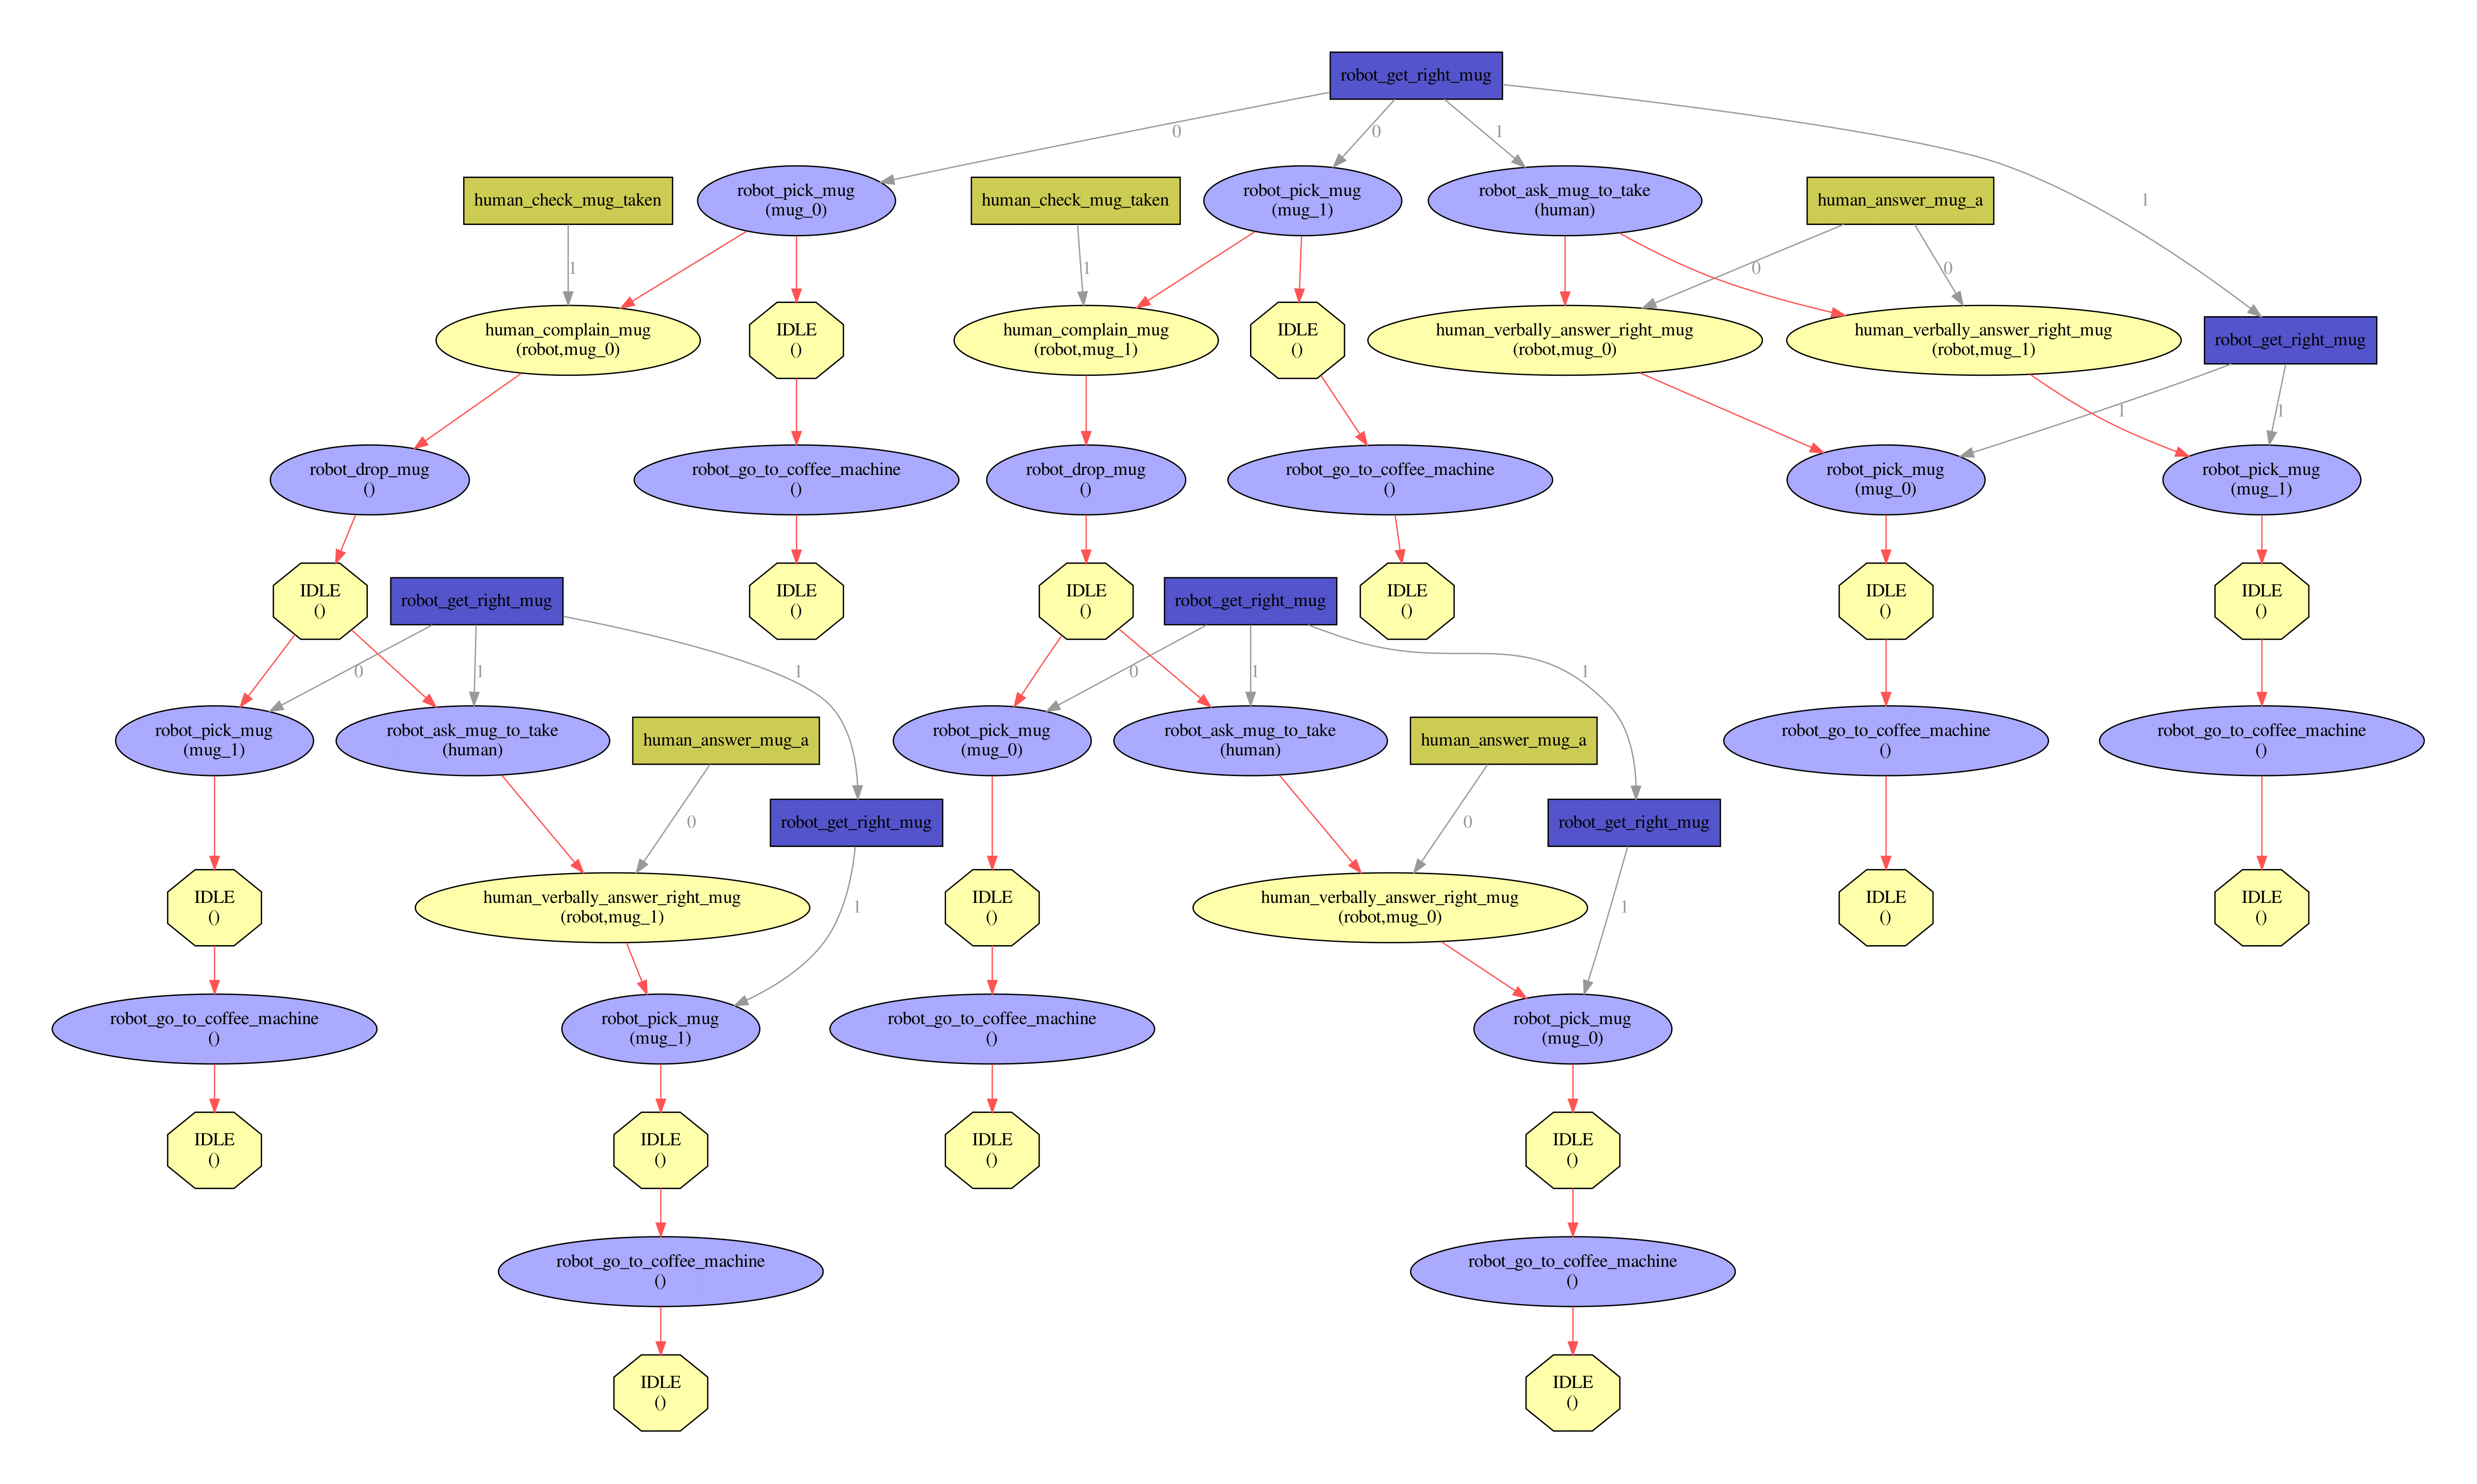
\includegraphics[width=\textwidth]{figures/chapter4/mug_selection_search_space.png}
\caption{CAPTION TODO}
\label{fig:chap4mugsss}
\end{figure}
\improvement{where can I introduce how to read this graph?}

The search space for $n=2$ mugs is presented in Figure~\ref{fig:chap4mugsss}. In this example, both mugs are distinct and RE can be computed. On the right hand side of the figure is the decomposition where the robot explicitly asks the human to designate her mug. The answer can either be \verb'mug_0' or \verb'mug_1'. The robot then pick the right one and go to the coffee machine, leaving no task to decompose.
On the left hand side of the figure is the decomposition where the robot proceeds via trials and errors. The robot can either pick \verb'mug_0' or \verb'mug_1' and the human will either react by doing nothing (if the robot took the right mug) or by complaining, in which case the robot will drop the mug, take the other one, and leave. Interestingly, we model the human reaction such as not expecting her to complain when taking the second mug after a first failure.

Next, we will compare different action costs and conditional plan selection criteria based on the same search space. To select a plan we used the Algorithm~\ref{alg:minaverage}. First, we set the cost of \verb'complain_mug' action much lower than the \verb'verbally_answer_right_mug' action. Here, the costs might have been set by the supervision component, estimating we are interacting in a noisy environment, where verbal communications are difficult to make, or that the human does not bother to correct the robot. The conditional plan returned is presented in Figure~\ref{fig:chap4mugtrialerror}. The chosen plan is the one containing trials and errors. Indeed, as it can lead to much shorter and thus less costly plans, it is the minimum average. 
\todo{caption}
\begin{figure}[hbtp]
\centering
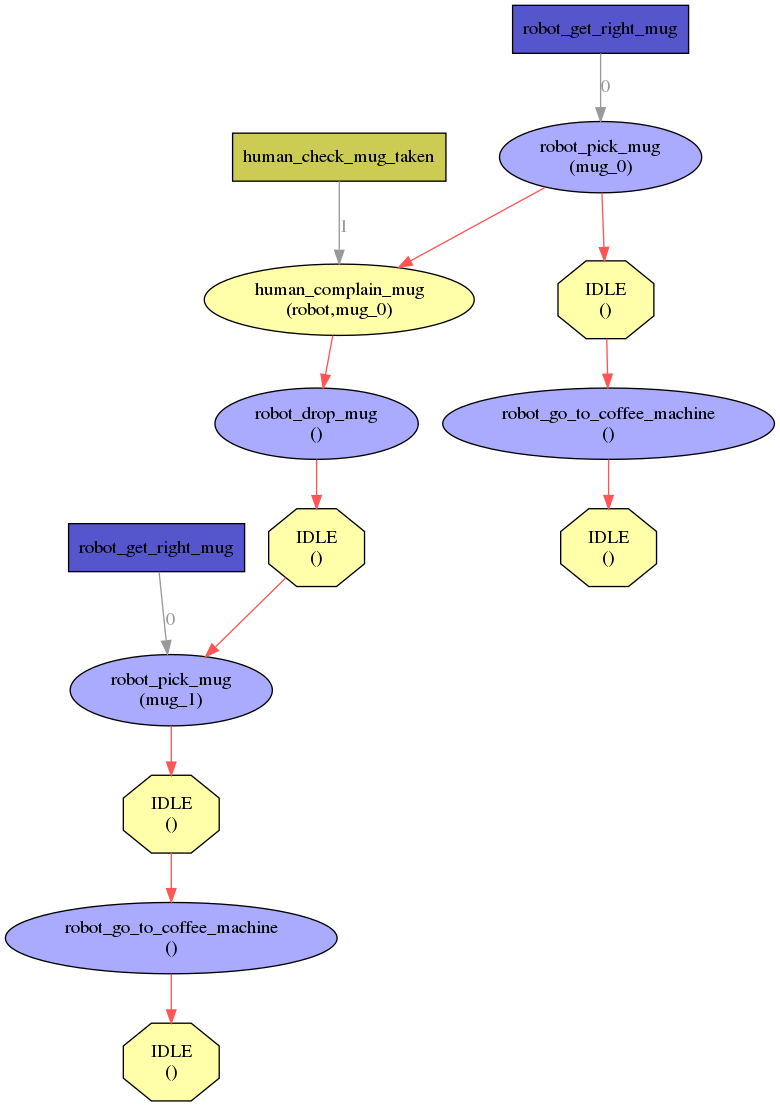
\includegraphics[width=0.8\textwidth]{figures/chapter4/mug_selection_trials.png}
\caption{CAPTION TODO}
\label{fig:chap4mugtrialerror}
\end{figure}

However, imagine that the human (who has still not had her coffee) is in a hurry, or that the mugs are really easy to distinguish from one another (\textit{e.g.} different color) and thus, we decrease the cost of the \verb'verbally_answer_right_mug' action and increase the cost of the \verb'complain_mug' action. The conditional plan selected is presented in Figure~\ref{fig:chap4mugask}. The robot know, prefers to ask for the right mug rather than trying to pick one at random.
\todo{caption}
\begin{figure}[hbtp]
\centering
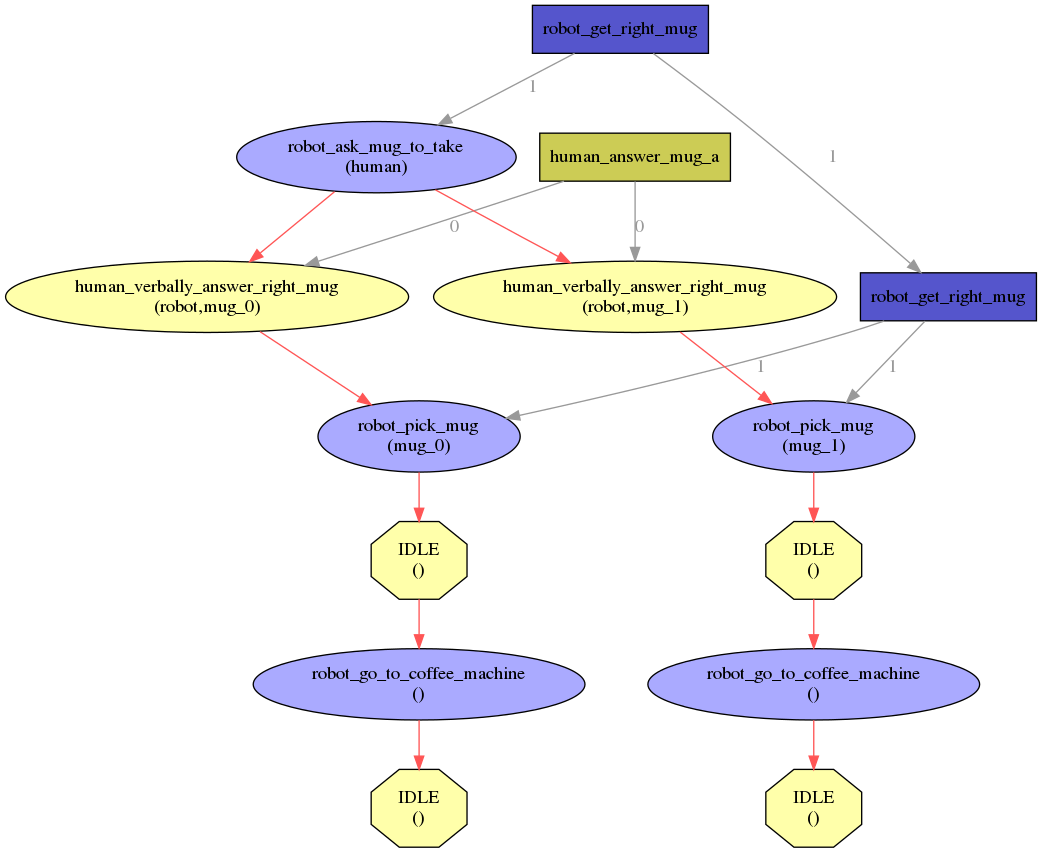
\includegraphics[width=\textwidth]{figures/chapter4/mug_selection_ask.png}
\caption{CAPTION TODO}
\label{fig:chap4mugask}
\end{figure}

As we increase the number of mugs $n$, the cost of \verb'verbally_answer_right_mug' has to also increase to make the robot choose the trials and errors decomposition, as the average of this decomposition increases since the number of potential errors increases. 
%Finally, if we make two mugs for which the REG does not find any solution (the mugs are not distinguishable from one another) the planner is able to generate conditional plans where it first tries to <-- not true for now, as we do not take into account failed actions in cost computation....

\improvement{Adds compute time for n=2,3,4,5}

\improvement{Add link to domain}

In this example we show one really interesting feature of our planner: representing human knowledge that is not known by the robot. While not being tractable when there are a lot of possibilities, it allows to select more or less conservative conditional plans depending on the cost of each actions. Moreover, this example allowed to see how updating the human agenda and how triggers can be used to model the agents interaction in the HTNs planning.
However, the human model was pretty simple, and we propose to challenge our planner in the next example with a task where the human is more involved.

\subsection{Balance difficult communications, decomposition cost and task attribution}
The robot is now heading to the coffee machine with the right mug in its gripper. On its way it detects another human taking a break near the coffee machine. The coffee has to be made. To brew coffee, ground coffee and water must be put in the coffee machine, and then the coffee can be served. While water is considered as always available, ground coffee is not. There are two places where ground coffee can be retrieved: either in the kitchen cupboard (close to the coffee machine) or in the pantry cupboard. 

\subsubsection{Handling the robot only case}
\label{subsubsec:chap4coffeerobotonly}
 First, we want the robot to be able to make coffee by itself, without requiring human help. To do so, we implement the following abstract tasks tree in the robot model (here we prepend the task names with \verb'r' where task are different in the robot and the human model):

\begin{itemize}
\item \verb'r_make_coffee' only having one decomposition (for now):
	\begin{itemize}
	\item \verb'r_make_coffee_alone' returning, in both orders (to represent partially ordered task tree), the tasks \verb'get_water', \verb'pour_water_in_machine' and \verb'r_get_coffee', \verb'put_coffee_in_machine'. Only \verb'r_get_coffee' is an abstract task.
	\end{itemize}
\item \verb'r_get_coffee' representing the ways for the robot to obtain coffee. It has only one decomposition:
	\begin{itemize}
	\item the decomposition returns $()$ if the robot has already coffee in its gripper. Else, it selects the closest cupboard and returns \verb'r_pick_coffee' with it as parameter.
	\end{itemize}
\end{itemize}

The robot primitive tasks as are follow:
\begin{itemize}
\item \verb'get_water' returning $\bot$ if the robot is already holding something; updating the beliefs of all the agents in the room with the fact that the robot holds water otherwise.
\item \verb'pour_water_in_machine' updating all the agents in the room beliefs with the machine being filled with water.
\item \verb'r_pick_coffee' returning $\bot$ if the robot is already holding something or if the cupboard passed as parameter does not contains coffee (in the robot beliefs); updating the beliefs of all agents in the room with the fact the the robot holds coffee otherwise.
\item \verb'put_coffee_in_machine' updating all the agents in the room beliefs with the machine being filled with coffee.
\item \verb'r_serve_coffee' updating all the agents in the room with the mug being filled with coffee.
\end{itemize}

Now, for the initial conditions we set that the robot knows there is coffee in the kitchen cupboard (the closest) and we add two tasks in its agenda: \verb'r_make_coffee' and \verb'r_serve_coffee'. The human has nothing in its agenda. The two possible plans for this really simple case are presented in Figure~\ref{fig:chap4coffeesimple}(a) and (b). The plan selection would then choose one of the plan based on robot action costs.

\todo{caption}
\begin{figure}[hbtp]
\centering
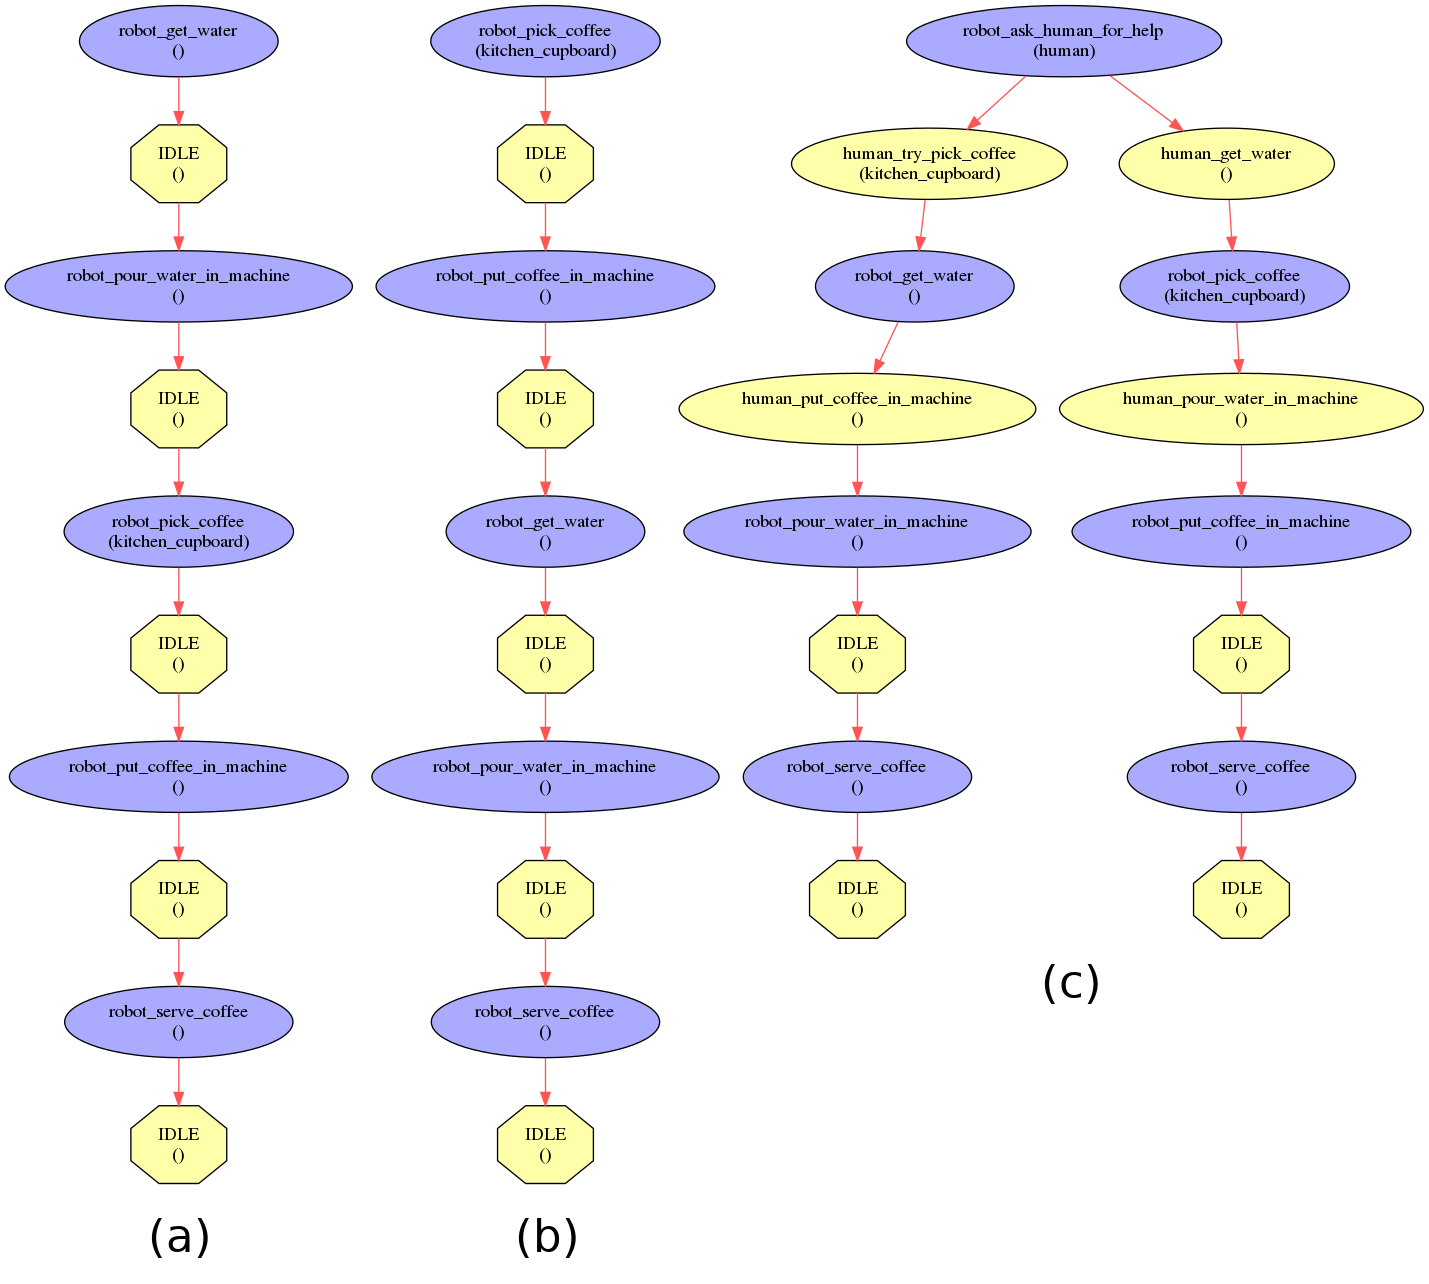
\includegraphics[width=\textwidth]{figures/chapter4/Chap4CoffeeSimplePlan.png}
\caption{CAPTION TODO}
\label{fig:chap4coffeesimple}
\end{figure}

\subsubsection{Incorporating the human planning process}
As we also want the robot to be able to ask the idling human to help it, we add, to its action model, a decomposition to the abstract task \verb'r_make_coffee' and a new abstract task \verb'help_make_coffee':

\begin{itemize}
\item \verb'r_make_coffee' containing the previous decomposition and the new one:
	\begin{itemize}
	\item \verb'r_make_coffee_collaboratively' returning the primitive task \verb'r_ask_human_for_help' and the abstract task \verb'r_help_make_coffee'
	\end{itemize}
\item \verb'help_make_coffee' representing the ways for the robot to help another agent to make coffee. It has only one decomposition:
	\begin{itemize}
	\item It returns \verb'get_water' and\verb'pour_water_in_machine' if there is no water in the machine and the human is doing a task related to bringing coffee. Likewise, it returns \verb'r_get_coffee' and \verb'put_coffee_in_machine' if there is no coffee in the machine and the human is doing a task related to fill the machine with water. Then, if the human is not doing any task, we add to the exploration \verb'r_get_coffee', \verb'put_coffee_in_machine' and \verb'help_make_coffee' if there is no coffee in the machine and \verb'get_water', \verb'pour_water_in_machine' and \verb'help_make_coffee'. The idea here is to complete the human actions if they take the initiative of a task, but to be proactive by exploring both possible alternatives if they are not. The recursion allows to reevaluate the need of this task later in the planning process.
	\end{itemize}
\end{itemize}

The primitive action added to the robot model is:
\begin{itemize}
\item \verb'r_ask_human_for_help' adding the task \verb'help_make_coffee' to the human agenda. Here we could have represented the possible refusal of the human by adding an abstract task leading to two possible decomposition for the human, accepting or declining, leading in similar schemes as in \ref{subsubsec:chap4coffeerobotonly}. However, to keep this example as simple as possible, we assume the human will always help the robot if asked to do so.
\end{itemize}

We model the human actions similarly to the robot ones. Their primitive tasks are defined as:
\begin{itemize}
\item \verb'help_make_coffee' representing the ways for the human to help another agent to make coffee. It has only one decomposition, which is the same as the robot one.
\item \verb'h_get_coffee' representing the ways for the human to obtain coffee. It has only one decomposition:
	\begin{itemize}
	\item the decomposition returns $()$ if the human is already holding coffee. Else, it selects the closest cupboard and returns \verb'h_try_pick_coffee' with it as parameter and \verb'h_get_coffee'. It differs from the robot one, indeed, whereas the knowledge of the robot is assumed to be the world state, the human's one can be false. Thus, the human might try to perform \verb'h_try_pick_coffee' on a cupboard not containing coffee. We take this into account with the recursion of this abstract task, and with the primitive task \verb'h_try_pick_coffee' described hereafter.
	\end{itemize}
\end{itemize}

The model of the human primitive actions are:
\begin{itemize}
\item \verb'get_water' as defined for the robot
\item \verb'pour_water_in_machine' as defined for the robot
\item \verb'h_try_pick_coffee' differs from the one defined for the robot as it checks if the cupboard passed as parameter really contains coffee (\textit{i.e.} in the robot beliefs). If it does not, the human's beliefs about this cupboard are updated to match the robot ones (modeling the human going in front of the cupboard, opening it and seeing the absence of coffee). If the cupboard does contain coffee in the robot beliefs, all the agents in the room beliefs are updated with the human having coffee in their hand.
\item \verb'put_coffee_in_machine' as defined for the robot.
\end{itemize}

The initial conditions are the same as presented before, but we also add that the kitchen cupboard contains coffee in the human beliefs. In addition to the two plans where the robot does not seek help to the human, another valid plan is found. This plan is presented in Figure~\ref{fig:chap4coffeesimple}(c). This conditional plan has two alternatives, depending on the initiative taken by the human.

\subsubsection{Updating human beliefs}
We can also change the initial conditions to elicit new behaviors. We keep the same action models for both the robot and the human, but we change the estimation of the human beliefs given as initial conditions to the planner. In a real robotic architecture, the human knowledge base would be updated with an estimation provided by situation assessment components. We specify that the human believes that both the kitchen and the pantry cupboard contain coffee. However, the robot knows (\textit{e.g.} using specific sensors or having been told about) that there is coffee only in the pantry cupboard. With these conditions, the search space extends to the three plans presented in Figure~\ref{fig:chap4coffeesimple}(a), (b), being when the robot prepare the coffee by itself, and in Figure~\ref{fig:chap4beliefsdiv}(a). In this last plan, we indeed model that the human will tend to first go to the nearest cupboard he thinks contains coffee. If this cupboard does not contain coffee, he will go to the next one. We can also note that only the left branch of the plan in Figure~\ref{fig:chap4beliefsdiv}(a) is impacted by this beliefs divergence. However, this branch choice is not up to the robot without any communication as we modeled the human as having the initiative of selecting a task. This subtlety cannot be represented in HATP.

Depending on the cost of the human being deceived and of the actions, the plan selected can be that the robot does all the task, as the human "mistake" can increase too much the average cost.

\todo{caption}
\begin{figure}[hbtp]
\centering
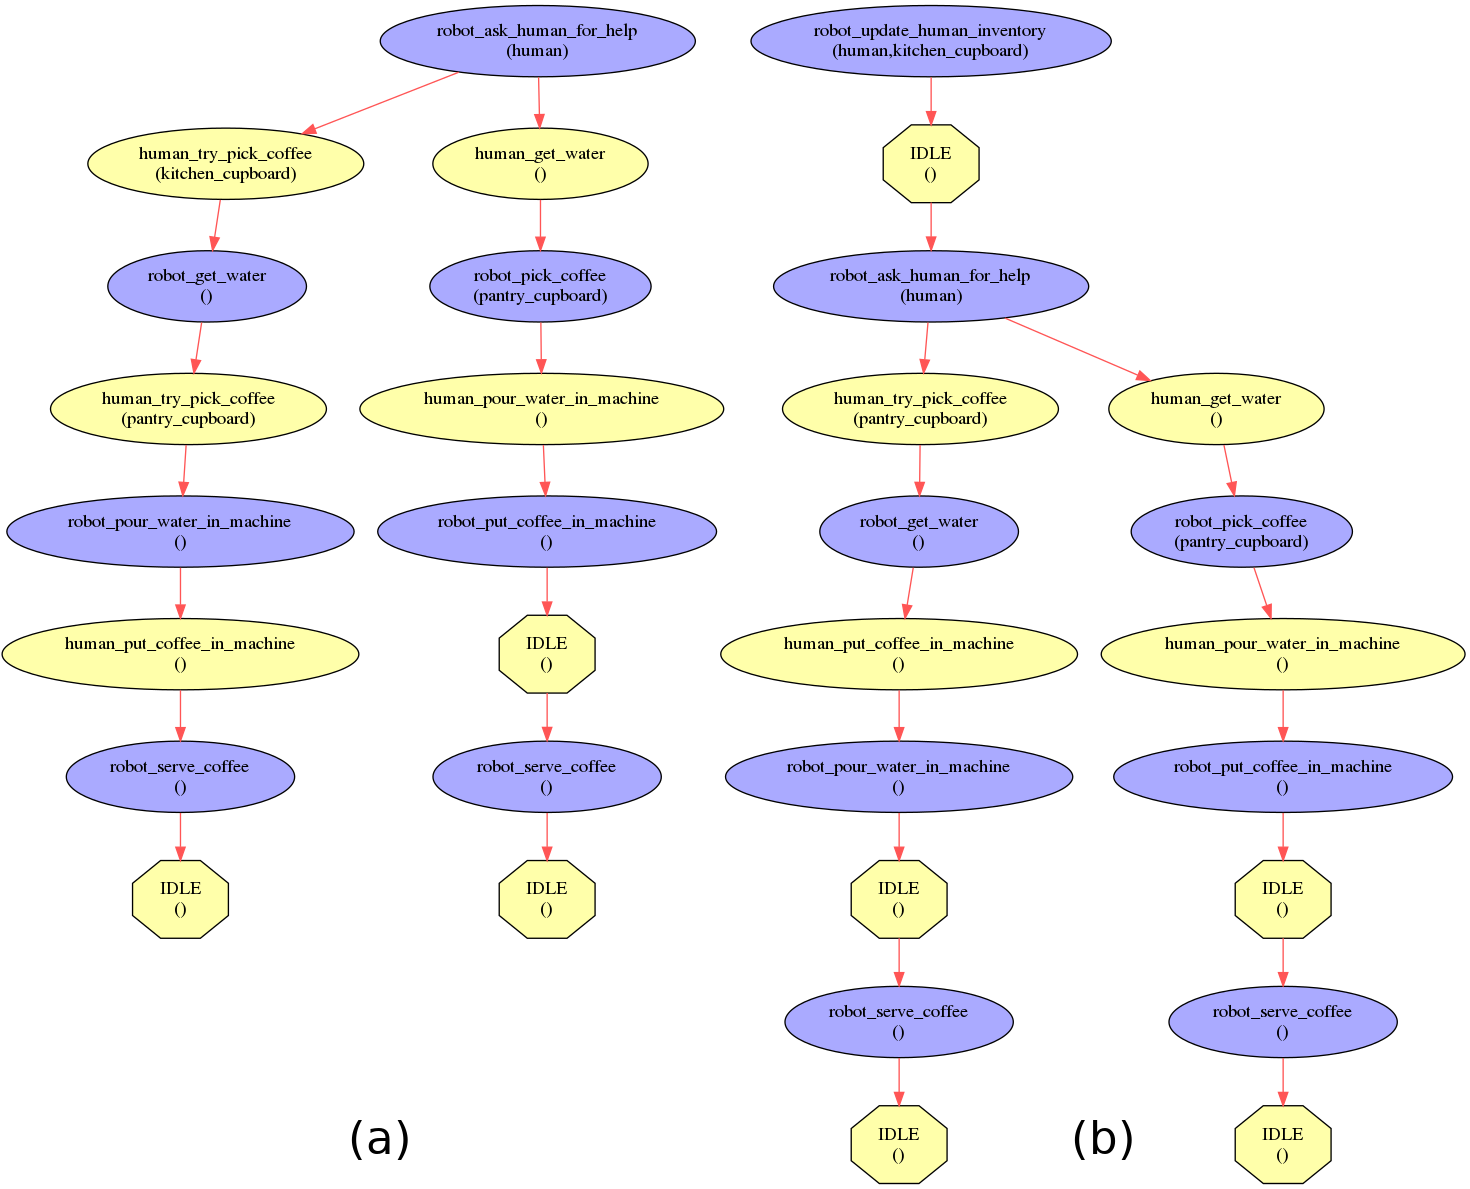
\includegraphics[width=\textwidth]{figures/chapter4/Chap4CoffeeBeliefDiv.png}
\caption{CAPTION TODO}
\label{fig:chap4beliefsdiv}
\end{figure}

To improve our robot, we want to make it able to realign the beliefs of the human, so, whatever the task he chooses, he will not make a mistake. To do so, we add a third decomposition to the \verb'r_make_coffee' abstract task and one new primitive task to the robot models.
\begin{itemize}
\item \verb'r_make_coffee' containing the previous two decompositions and the new one:
	\begin{itemize}
	\item \verb'r_align_and_make_coffee_collaboratively' returning $\bot$ if no belief divergence is detected between the robot and the human. The decomposition returns the new primitive task \verb'r_update_human_inventory' along with \verb'r_ask_human_for_help' and \verb'r_help_make_coffee'. An alternative for \verb'r_update_human_inventory' is returned with as parameter each cupboard in diverging beliefs between the robot and the human.
	\end{itemize}
\item \verb'r_update_human_inventory' being a primitive task. It updates the human beliefs concerning the cupboard passed as parameter with the beliefs of the robot.
\end{itemize}

With this new decomposition the new plan presented in Figure~\ref{fig:chap4beliefsdiv}(b) is added to the search space. In this plan the human beliefs are updated before asking him to help the robot to make coffee. The human does not make the mistake of going first to the kitchen cupboard.

Depending on the communication cost (estimated using the REG approach presented in the previous chapter), the human deception cost and the other actions costs any one of the four possible plans can be selected. For example, to minimize the human involvement and if the communication has a high cost, the selected plan would be Figure~\ref{fig:chap4coffeesimple}(a) or (b). If the communication is costly but the pantry and kitchen cupboard are not too far away, the selected plan is Figure~\ref{fig:chap4beliefsdiv}(a), finally, if we represent that the human would be upset if he makes a mistake or if the communication for aligning beliefs is not expensive, the plan Figure~\ref{fig:chap4beliefsdiv}(b) would be returned.

Through all these examples we show that this task planning approach, which separates human and robot beliefs and action models, can be suitable for multiple problems. We are able to plan for robot unknown human beliefs, to rely on the human planning process while keeping inherent uncertainties (\textit{i.e.} not making choices for them, without communicating them) and also to plan diverging beliefs and balance the actions of realigning them with plans containing mistakes. In the next section, we present a HRI task, inspired from psychology, that has never been tackled in robotics and we show how our planner is integrated in a fully functional robotic architecture dedicated for this task.


\section{The Director Task}

\section{Conclusion and Future Works}
\subsection{Representing explicitly observation processes}

\subsection{Leveling-up the theory of mind}

\subsection{Pruning during the search space exploration}

\ifdefined\included
\else
\bibliographystyle{acm}
\bibliography{These}
\end{document}
\fi

\ifdefined\included
\else
\documentclass[a4paper,11pt,twoside]{StyleThese}
\usepackage{amsmath,amssymb, amsthm}             % AMS Math
\usepackage[T1]{fontenc}
\usepackage[utf8x]{inputenc}
\usepackage{babel}
\usepackage{datetime}

\usepackage{silence}

\WarningFilter{minitoc(hints)}{W0023}
\WarningFilter{minitoc(hints)}{W0028}
\WarningFilter{minitoc(hints)}{W0030}

\usepackage{lmodern}
\usepackage{tabularx}
%\usepackage{tabular}
\usepackage{multirow}
\usepackage{xspace}

\usepackage{hhline}
\usepackage[left=1.5in,right=1.3in,top=1.1in,bottom=1.1in,includefoot,includehead,headheight=13.6pt]{geometry}
\renewcommand{\baselinestretch}{1.05}

% Table of contents for each chapter

\usepackage[nottoc, notlof, notlot]{tocbibind}
\usepackage{minitoc}
\setcounter{minitocdepth}{2}
\mtcindent=15pt
% Use \minitoc where to put a table of contents

\usepackage{aecompl}

% Glossary / list of abbreviations

\usepackage[intoc]{nomencl}
\iftoggle{ThesisInEnglish}{%
\renewcommand{\nomname}{Glossary}
}{ %
\renewcommand{\nomname}{Liste des Abréviations}
}

\usepackage{etoolbox}
\renewcommand\nomgroup[1]{%
  \item[\bfseries
  \ifstrequal{#1}{A}{Number Sets}{%
  \ifstrequal{#1}{G}{Agents Beliefs and Action Models}{%
  \ifstrequal{#1}{N}{Navigation}{%
  \ifstrequal{#1}{O}{Ontology}{%
  \ifstrequal{#1}{R}{Referring Expression Generation}{%
  \ifstrequal{#1}{Z}{Controllable and Uncontrollable Agents Task Planning}{}}}}}}%
]}

\makenomenclature



% My pdf code

\usepackage{ifpdf}

\ifpdf
  \usepackage[pdftex]{graphicx}
  \DeclareGraphicsExtensions{.jpg}
  \usepackage[pagebackref,hyperindex=true]{hyperref}
  \usepackage{tikz}
  \usetikzlibrary{arrows,shapes,calc}
\else
  \usepackage{graphicx}
  \DeclareGraphicsExtensions{.ps,.eps}
  \usepackage[dvipdfm,pagebackref,hyperindex=true]{hyperref}
\fi

\graphicspath{{.}{images/}}

%% nicer backref links. NOTE: The flag ThesisInEnglish is used to define the
% language in the back references. Read more about it in These.tex

\iftoggle{ThesisInEnglish}{%
\renewcommand*{\backref}[1]{}
\renewcommand*{\backrefalt}[4]{%
\ifcase #1 %
(Not cited.)%
\or
(Cited in page~#2.)%
\else
(Cited in pages~#2.)%
\fi}
\renewcommand*{\backrefsep}{, }
\renewcommand*{\backreftwosep}{ and~}
\renewcommand*{\backreflastsep}{ and~}
}{%
\renewcommand*{\backref}[1]{}
\renewcommand*{\backrefalt}[4]{%
\ifcase #1 %
(Non cité.)%
\or
(Cité en page~#2.)%
\else
(Cité en pages~#2.)%
\fi}
\renewcommand*{\backrefsep}{, }
\renewcommand*{\backreftwosep}{ et~}
\renewcommand*{\backreflastsep}{ et~}
}

% Links in pdf
\usepackage{color}
\definecolor{linkcol}{rgb}{0,0,0.4} 
\definecolor{citecol}{rgb}{0.5,0,0} 
\definecolor{linkcol}{rgb}{0,0,0} 
\definecolor{citecol}{rgb}{0,0,0}
% Change this to change the informations included in the pdf file

\hypersetup
{
bookmarksopen=true,
pdftitle="Planning For Both Robot and Human: Anticipating and Accompanying Human Decisions",
pdfauthor="Guilhem BUISAN", %auteur du document
pdfsubject="Thèse", %sujet du document
%pdftoolbar=false, %barre d'outils non visible
pdfmenubar=true, %barre de menu visible
pdfhighlight=/O, %effet d'un clic sur un lien hypertexte
colorlinks=true, %couleurs sur les liens hypertextes
pdfpagemode=None, %aucun mode de page
pdfpagelayout=SinglePage, %ouverture en simple page
pdffitwindow=true, %pages ouvertes entierement dans toute la fenetre
linkcolor=linkcol, %couleur des liens hypertextes internes
citecolor=citecol, %couleur des liens pour les citations
urlcolor=linkcol %couleur des liens pour les url
}

% definitions.
% -------------------

\setcounter{secnumdepth}{3}
\setcounter{tocdepth}{2}

% Some useful commands and shortcut for maths:  partial derivative and stuff

\newcommand{\pd}[2]{\frac{\partial #1}{\partial #2}}
\def\abs{\operatorname{abs}}
\def\argmax{\operatornamewithlimits{arg\,max}}
\def\argmin{\operatornamewithlimits{arg\,min}}
\def\diag{\operatorname{Diag}}
\newcommand{\eqRef}[1]{(\ref{#1})}

\usepackage{rotating}                    % Sideways of figures & tables
%\usepackage{bibunits}
%\usepackage[sectionbib]{chapterbib}          % Cross-reference package (Natural BiB)
%\usepackage{natbib}                  % Put References at the end of each chapter
                                         % Do not put 'sectionbib' option here.
                                         % Sectionbib option in 'natbib' will do.
\usepackage{fancyhdr}                    % Fancy Header and Footer

% \usepackage{txfonts}                     % Public Times New Roman text & math font
  
%%% Fancy Header %%%%%%%%%%%%%%%%%%%%%%%%%%%%%%%%%%%%%%%%%%%%%%%%%%%%%%%%%%%%%%%%%%
% Fancy Header Style Options

\pagestyle{fancy}                       % Sets fancy header and footer
\fancyfoot{}                            % Delete current footer settings

%\renewcommand{\chaptermark}[1]{         % Lower Case Chapter marker style
%  \markboth{\chaptername\ \thechapter.\ #1}}{}} %

%\renewcommand{\sectionmark}[1]{         % Lower case Section marker style
%  \markright{\thesection.\ #1}}         %

\fancyhead[LE,RO]{\bfseries\thepage}    % Page number (boldface) in left on even
% pages and right on odd pages
\fancyhead[RE]{\bfseries\nouppercase{\leftmark}}      % Chapter in the right on even pages
\fancyhead[LO]{\bfseries\nouppercase{\rightmark}}     % Section in the left on odd pages

\let\headruleORIG\headrule
\renewcommand{\headrule}{\color{black} \headruleORIG}
\renewcommand{\headrulewidth}{1.0pt}
\usepackage{colortbl}
\arrayrulecolor{black}

\fancypagestyle{plain}{
  \fancyhead{}
  \fancyfoot{}
  \renewcommand{\headrulewidth}{0pt}
}

%\usepackage{MyAlgorithm}
%\usepackage[noend]{MyAlgorithmic}
\usepackage{algorithm}
\usepackage[noend]{algpseudocode}
\usepackage{comment}
\usepackage[ED=EDSYS-Robo, Ets=INSA]{tlsflyleaf}
%%% Clear Header %%%%%%%%%%%%%%%%%%%%%%%%%%%%%%%%%%%%%%%%%%%%%%%%%%%%%%%%%%%%%%%%%%
% Clear Header Style on the Last Empty Odd pages
\makeatletter

\def\cleardoublepage{\clearpage\if@twoside \ifodd\c@page\else%
  \hbox{}%
  \thispagestyle{empty}%              % Empty header styles
  \newpage%
  \if@twocolumn\hbox{}\newpage\fi\fi\fi}

\makeatother
 
%%%%%%%%%%%%%%%%%%%%%%%%%%%%%%%%%%%%%%%%%%%%%%%%%%%%%%%%%%%%%%%%%%%%%%%%%%%%%%% 
% Prints your review date and 'Draft Version' (From Josullvn, CS, CMU)
\newcommand{\reviewtimetoday}[2]{\special{!userdict begin
    /bop-hook{gsave 20 710 translate 45 rotate 0.8 setgray
      /Times-Roman findfont 12 scalefont setfont 0 0   moveto (#1) show
      0 -12 moveto (#2) show grestore}def end}}
% You can turn on or off this option.
% \reviewtimetoday{\today}{Draft Version}
%%%%%%%%%%%%%%%%%%%%%%%%%%%%%%%%%%%%%%%%%%%%%%%%%%%%%%%%%%%%%%%%%%%%%%%%%%%%%%% 

\newenvironment{maxime}[1]
{
\vspace*{0cm}
\hfill
\begin{minipage}{0.5\textwidth}%
%\rule[0.5ex]{\textwidth}{0.1mm}\\%
\hrulefill $\:$ {\bf #1}\\
%\vspace*{-0.25cm}
\it 
}%
{%

\hrulefill
\vspace*{0.5cm}%
\end{minipage}
}

\let\minitocORIG\minitoc
\renewcommand{\minitoc}{\minitocORIG \vspace{1.5em}}

\usepackage{multirow}
%\usepackage{slashbox}

\newenvironment{bulletList}%
{ \begin{list}%
	{$\bullet$}%
	{\setlength{\labelwidth}{25pt}%
	 \setlength{\leftmargin}{30pt}%
	 \setlength{\itemsep}{\parsep}}}%
{ \end{list} }

\theoremstyle{definition}
\newtheorem{definition}{Definition}
\renewcommand{\epsilon}{\varepsilon}

% centered page environment

\newenvironment{vcenterpage}
{\newpage\vspace*{\fill}\thispagestyle{empty}\renewcommand{\headrulewidth}{0pt}}
{\vspace*{\fill}}

\usepackage{tablefootnote}

\theoremstyle{plain}
\newtheorem{constraint}{Constraint}[section]

\algnewcommand\algorithmicforeach{\textbf{for each}}
\algnewcommand\algorithmicin{\textbf{in}}
\algdef{S}[FOR]{ForEach}[2]{\algorithmicforeach\ #1\ \algorithmicin\ #2\ \algorithmicdo}

\usepackage{listings}
\lstdefinestyle{customPlan}{
  language=C,
  commentstyle=\itshape\color{green!25!black},
}
\usepackage{pdfpages}

\sloppy
\begin{document}
\fi


\chapter*{Conclusion}
\addstarredchapter{Conclusion} %Sinon cela n'apparait pas dans la table des matières
\markboth{CONCLUSION}{}

In this thesis we presented several contributions focusing on endowing the robot with ability to plan explicity for itslef and for the human. Indeed, several approaches to human-aware navigation planning (and motion planning in general) account for human presence by including social costs influencing the trajectory, but only plan a course of actions for the robot. While being successful when humans are static or when evolving in large environment, these approaches are challenged when the interaction becomes intricate, where the robot and the human must collaborate to solve a problem. In robotic task planning, where human robot intricate interactions are easier to explore, some approaches do include planning for both the human and the robot. However, these approaches seldom maintain different beliefs for both agents during the planning process, whereas it is what a human is expecting according to joint action theory. Moreover, these approaches consider the human as a totally controllable agent, close to what is done in multi robot planning. They do not account for communications needed to align beliefs or to share the plan.

In Chapter~\ref{chapter:navigation}, we showed why planning for both the human and the robot is important for navigation planning in intricate interaction scenarios. Not only it allows to find valid solutions where other approaches would have not, but, by anticipating the possible human trajectory we can make the robot more efficient and its behavior more satisfactory for the human.  Indeed, by estimating the human future positions and speed, we are able to make the robot trajectory less threatening, more legible and to enhance the mutual manifestness of the robot. These results were validated through a user study, involving a totally autonomous PR2 robot crossing a human in a narrow corridor. We also presented how this navigation scheme has been implemented on other robots, including a HRP2 humanoid robot and a Pepper robot which has been deployed autonomously for several weeks providing route description to customers in a mall.

Alleviating from ephemeral nature of human robot navigation interaction, we presented a new way of planning for communication during task planning in Chapter~\ref{chapter:comm}. We chose to make a hybrid planning approach where a domain-independent HTN planner (HATP) delegates the resolution of feasibility and cost of communication actions to a domain-specific communication planner. We focused on communication actions needing to designate objects to the other agent. Thus, we needed a domain-specific planner able to determine the content of such communications. This problem is called referring expression generation and, albeit studied for a long time, we did not find any suitable existing work to be integrated in a human robot task planning scheme. Indeed, to be used in task planning, such a planner must be efficient and some specific constraints imposed by human robot interaction have to be satisfied. We formalized the REG problem for HRI using an ontology as a knowledge base and we proposed an efficient algorithm to solve it. This algorithm has been shown to be the most efficient to our knowledge while being designed for HRI scenarios. It then has been integrated in HATP, an HTN planner able to maintain beliefs of multiple agents during task planning. Resolving the content of communication actions at this stage is only doable if the planner plans for both human and robot, it allows to prevent to reach situations where the execution is blocked because a communication action cannot be performed and also improve the quality of plans.

However, HATP relies on exploring only one hierarchical task network (HTN) and allocate task to either the robot or the human depending on the task constraints to find an optimal plan. Representing interactive tasks this way leads to execution where the human is considered as knowing the plan before it begins. Indeed, several works use similar approaches and solve contingencies (\textit{e.g.} beliefs divergence, plan communication) during the plan execution. 

In Chapter~\ref{chapter:doublehtn} we propose a new task planning scheme enriching current human-aware task planners. The general idea is to not only keep distinct beliefs between the robot and the human but also have two separated action models. Both models are HTNs, but do not represent the same concepts. The robot HTN, as in classical HTN planning, is designed to give expert knowledge to the planner on the different ways for the robot to perform a task. The human HTN on the other hand, is closer to a human task model as used in interactive systems engineering in human computer interaction. It aims at representing how a human may achieve a task (\textit{i.e.} emulating parts of their planning process) and how they may react to a particular world state or to a robot request. The presented planner uses both HTNs to elaborate valid conditional plans then selects the optimal one. These conditional plans contain the possible human actions deduced via their task model. We presented our approach in scenarios involving intricate human robot interactions and showed how it is suitable and results in interesting plans. 

Finally, in Chapter~\ref{chapter:integration}, we presented how this new task planning scheme can be integrated into a complete robotic architecture dedicated to HRI. Moreover, we introduced a new task for HRI inspired from psychology experiments along with an implemented robotic architecture including our planning scheme, allowing to tackle some of the challenges of this task.

\section*{On the human agent interaction guidelines and joint action theory principles}
\markright{HUMAN-AGENT INTERACTION GUIDELINES}
We presented in Chapter~\ref{chapter:sota} maxims coined by Bradshaw \textit{et al.}~\cite{bradshaw2011human} for human-agent interaction. We propose here to sum up which maxims have guided the work presented in this thesis and to what extent we were able to implement them.

By completely exploring the search space with the proposed planning method of Chapter~\ref{chapter:doublehtn}, we can increase the \textit{progress appraisal} of the robot. Indeed, by returning all the conditional plan to the supervision it can compute how much the task is progressing, and communicate it to the human if needed. Besides, we proposed a plan post-processing step where robot actions are added to guide human actions away from potential errors and to the optimal plan.

Moreover, by explicitly representing the action effects in the beliefs of both agent, we explicitly represent the \textit{observability} of the robot. Moreover, as we consider some effects (or even some actions) to be not observable, and thus, not updating the human beliefs, the robot observability will impact the elaborated plan.

Then, we showed our approach can be used to balance plans where the robot is proactive and ones where it let the human choose the tasks attributions. This matches to the agent \textit{knowing its limits} maxim. Moreover, unlike HATP, the human decisions are not set, the planner provide a robot course of action for multiple possible human actions, thus adapting to the human choices. We also envision to use the HTNs exploration to guide the human choices or inform them about potential outcomes.

Moreover, by representing robot unknown human beliefs, the robot is able to plan to ask question and predict possible human answers to them, making the robot more \textit{directable}. A strong link between the task planning process and the supervision is required to explore further this maxim.

Similarly, a first step has been made towards the negotiation and deconfliction of plans and beliefs alignment, increasing the robot \textit{coordination}. Some possible approaches where presented in Chapter~\ref{chapter:doublehtn} to increase it even more by interacting with the human during the plan elaboration process, in addition to the human planing process emulation. This also requires a stronger link with supervision, currently being explored.

Besides, we allowed to make the robot more \textit{selective} as we showed in Chapter~\ref{chapter:doublehtn}, by allowing to plan belief alignment actions only when they are needed, and only with the beliefs required by the human to perform better.

Finally, we showed in Chapter~\ref{chapter:navigation} that planning navigation for both the human and the robot allows to make the robot deconflict the trajectories earlier increasing the robot \textit{predictability}. Moreover, we implemented a head behavior for the navigation aiming at showing its future trajectory while acknowledging the human presence.

\section*{Limitations and future work}
\markright{LIMITATIONS AND FUTURE WORK}
We think there is plenty of potential for the task planning approach presented in Chapter~\ref{chapter:doublehtn} and it must be refined and enriched. While it seems promising, as it allows to represent and find plans for intricate interaction scenarios, has been integrated with a domain-specific communication planner and used into a robotic architecture, limitations can be identified. First, the turn-taking approach used does not translate the duration of actions. Indeed, some actions will be longer than others, and not accounting for it may lead to suboptimal plans and wrong prediction of human actions. Then, by not pruning some part of the exploration graph during the search, the approach is not efficient for large HTN domains. Efficiency can also by gained by a better implementation in C++ rather than in Python. However, pruning while searching would prevent applying plan-wide costs.


\subsection*{Bringing planning and supervision closer}
Some future work has already been identified to extend the approaches presented in this thesis. The first one, already mentioned before, is to build a stronger link with supervision. In common robotic architectures, the link between the supervision and geometric and task planning come down to planning request and plan response. However, this link may not be enough for long term interaction or intricate and dynamic situations usually found in HRI.

For HATEB, the navigation scheme presented in Chapter~\ref{chapter:navigation}, the solution proposed assumes the human will respect the model provided, and adjust the robot trajectory accordingly. For example, if the robot is following the human in a narrow corridor, if the human goes slower than what is set in the navigation planner parameters, the robot will never overtake them. Indeed, the planned trajectory for the human is for them to accelerate making the robot following the human permanently. The human model provided to the planner ($\humanmodel$) must be as accurate as possible. Providing a perfect model for each human encountered is obviously impossible, that is why the supervision must not only provide an initial model to the planner with the planning request but must also update this human model during the execution, especially if contingencies are detected to happen while following the plan. Here for example, a supervision system might decrease the human speed parameter if they are repeatedly detected to move slower than expected.

For the REG algorithm presented in Chapter~\ref{chapter:comm} this human model update is also crucial to have a good estimate of communication capabilities of the human and the associated difficulties to understand. As presented, some relations to describe an object are more difficult to understand than others. In our approach, we represented it by a cost associated to each properties. This difficulty depends on the person the robot is interacting with. For example, using color to refer to an object is less efficient or even impossible when speaking to a color blind person. Our costs are indeed defined per human we are interacting with. Besides, the difficulty to understand is also context dependent. For instance, colors relation can be hard or even impossible to perceive if the scene is lit with colored lights. Again, to cope with these issue, the supervision must update on the human model used for planning during the execution. Moreover, it can request and iterate with the planner during the planning process to allow for more or less risky communications, leading to more or less efficient plans.

The same is true for the planning approach depicted in Chapter~\ref{chapter:doublehtn}. The human action model along with associated costs must be updated on a per-human basis all along the interaction. By refining the human model the best prediction would be made for them, leading to more efficient plans. Besides, some task or actions can be enabled or disabled depending on the human and their level of expertise in the task and for robot collaboration. Heuristics can also be learned as to which decomposition a human may use for a task in a specific context. Highly probable decompositions can then be explored first, resulting in a more efficient planning process.

To reduce the branching factor in human HTN exploration, we can also try to negotiate the plan while elaborating it. For example, if too many human actions are returned during the search, the planning process can request the supervision to propose the different task alternatives to the human and ask which one they would perform in the specific state the planner is in. Only the answered alternatives can then be explored by the planner. Not only it would help reducing the branching factor, but the robot may appear more \textit{predictable} and the plan more \textit{explainable} as some actions would have been chosen by the human. Thanks to the HTN structure, communication about the tasks made easier. This negotiation may need multiple iterations as the alternatives proposed by the human may lead to unfeasible plans. However, if the choice is proposed for a point too far in the future, the human may have a hard time projecting themselves in that situation.

In addition to considering the possible human actions in the conditional plan, the planner could also expose the effects of the actions and more precisely the observable effects of them. By doing so, the supervision would know what to expect from the human and what to monitor to determine which action the human did, influencing the branch of the plan executed. Going further, the supervision may use the entire human action model to be able to also predict human behavior, in case of plan repair for example.

\subsection*{Theory of mind level up}
To make a better prediction of the human decisions and actions, some advanced scenarios require the robot to represent the model the human has made of it ($\robotinhumanmodel$). Indeed, as shown by Chakraborti \textit{et al.}~\cite{chakraborti2017plan}, using it can lead to more legible and predictable plans. As described in the Chapter~\ref{chapter:sota}, joint action theory informs about the capabilities a human is using when interacting with another agent. Especially, humans can \textit{predict} other's actions and \textit{integrate them into their own plan}. Thus, the model the human is making about the robot will influence their decision process and how they will perform a task. This is why it is important to build this model. One approach to do so is to analyze the actions performed by the robot by taking the perspective of the human and emulate an inferring process to build a robot model.

For example, in the navigation scheme from Chapter~\ref{chapter:navigation}, integrating this model would lead to a better prediction of human trajectory. The robot trajectory costs would also be more accurate, as more constraints could be added. A surprise cost for instance can be estimated by comparing the planned robot trajectory ($\robotmodel$), with the one expected by the human ($\robotinhumanmodel$). This could, in turn, be used to better respect and evaluate the respect of the maxim of \textit{predictability} and \textit{dependability}.

Likewise, in the planning approach presented in Chapter~\ref{chapter:doublehtn}, using the estimation of the robot model that the human has would result in more accurate predictions of human actions. Indeed, we know that the human will integrate actions of other agents in their own plan, as showed by joint action theory. Until now, we assumed that it would not be the case as we envisioned interaction with novice users who have never interacted with a robot before, or not enough to be confident to integrate the robot action in their planning process. But, as they would gain experience, trust and habits, human partners will expect the robot to perform in a certain way. Plans quality would increase by integrating these expectations in the emulation of human planning process. Moreover, we could improve the \textit{directability} and \textit{observability} of the robot by adding possible actions explicitly updating the human's robot model.


\ifdefined\included
\else
\bibliographystyle{acm}
\bibliography{These}
\end{document}
\fi

\nomenclature{$\robotmodel$}{The global model of the robot}

\newpage
\listoftodos[Notes]


\appendix

\chapter{Navigation User Study Questionnaires}
\label{annex:questionnaires}
\section[PeRDITA (French)]{Original PeRDITA Questionnaire Without Verbal Dimension (French)}
\begin{center}
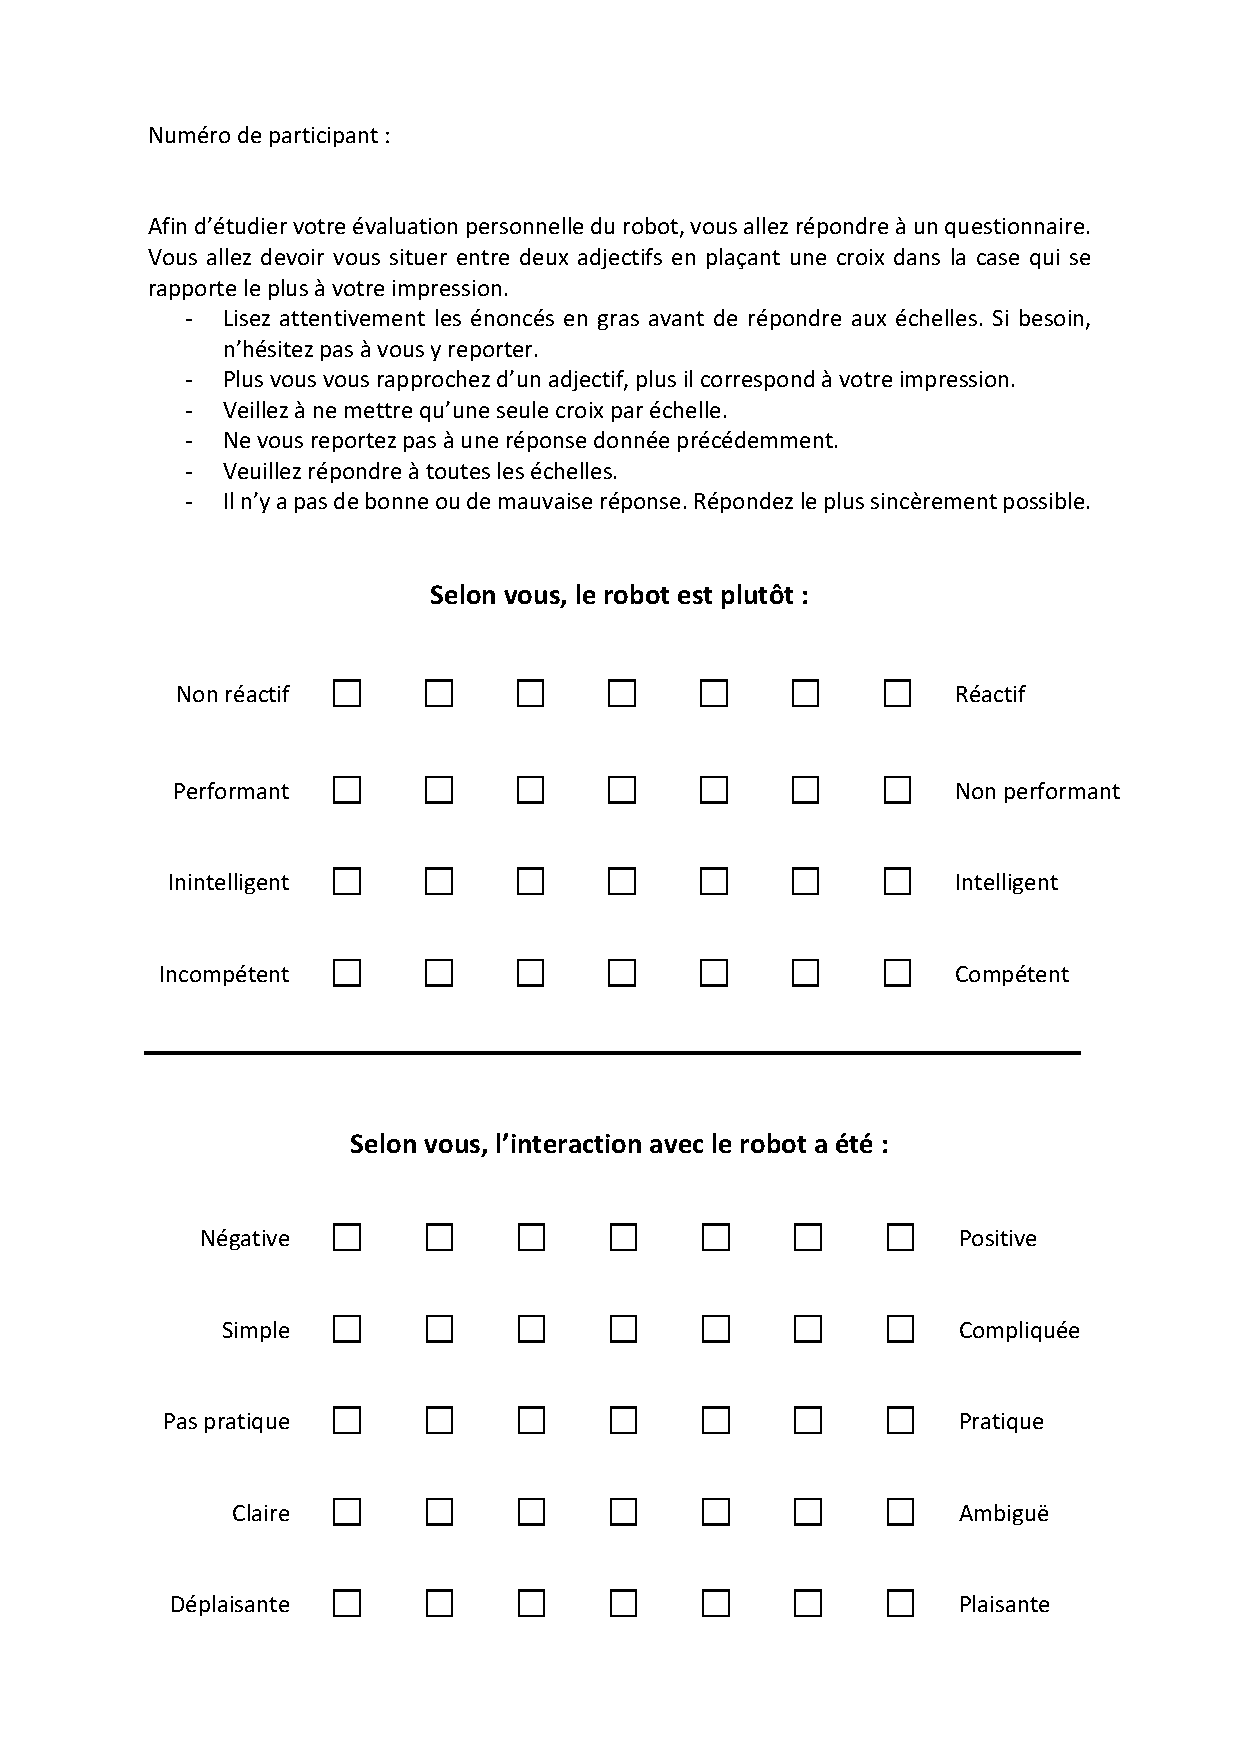
\includegraphics[page=1, width=\textwidth]{Annexes/PeRDITA_vParticipant_sansDimVerbale.pdf} 
\end{center}

\begin{center}
\includegraphics[page=2, width=\textwidth]{Annexes/PeRDITA_vParticipant_sansDimVerbale.pdf} 
\end{center}

\section[PeRDITA (Translated)]{Unofficial Translation of the PeRDITA Questionnaire}
\begin{center}
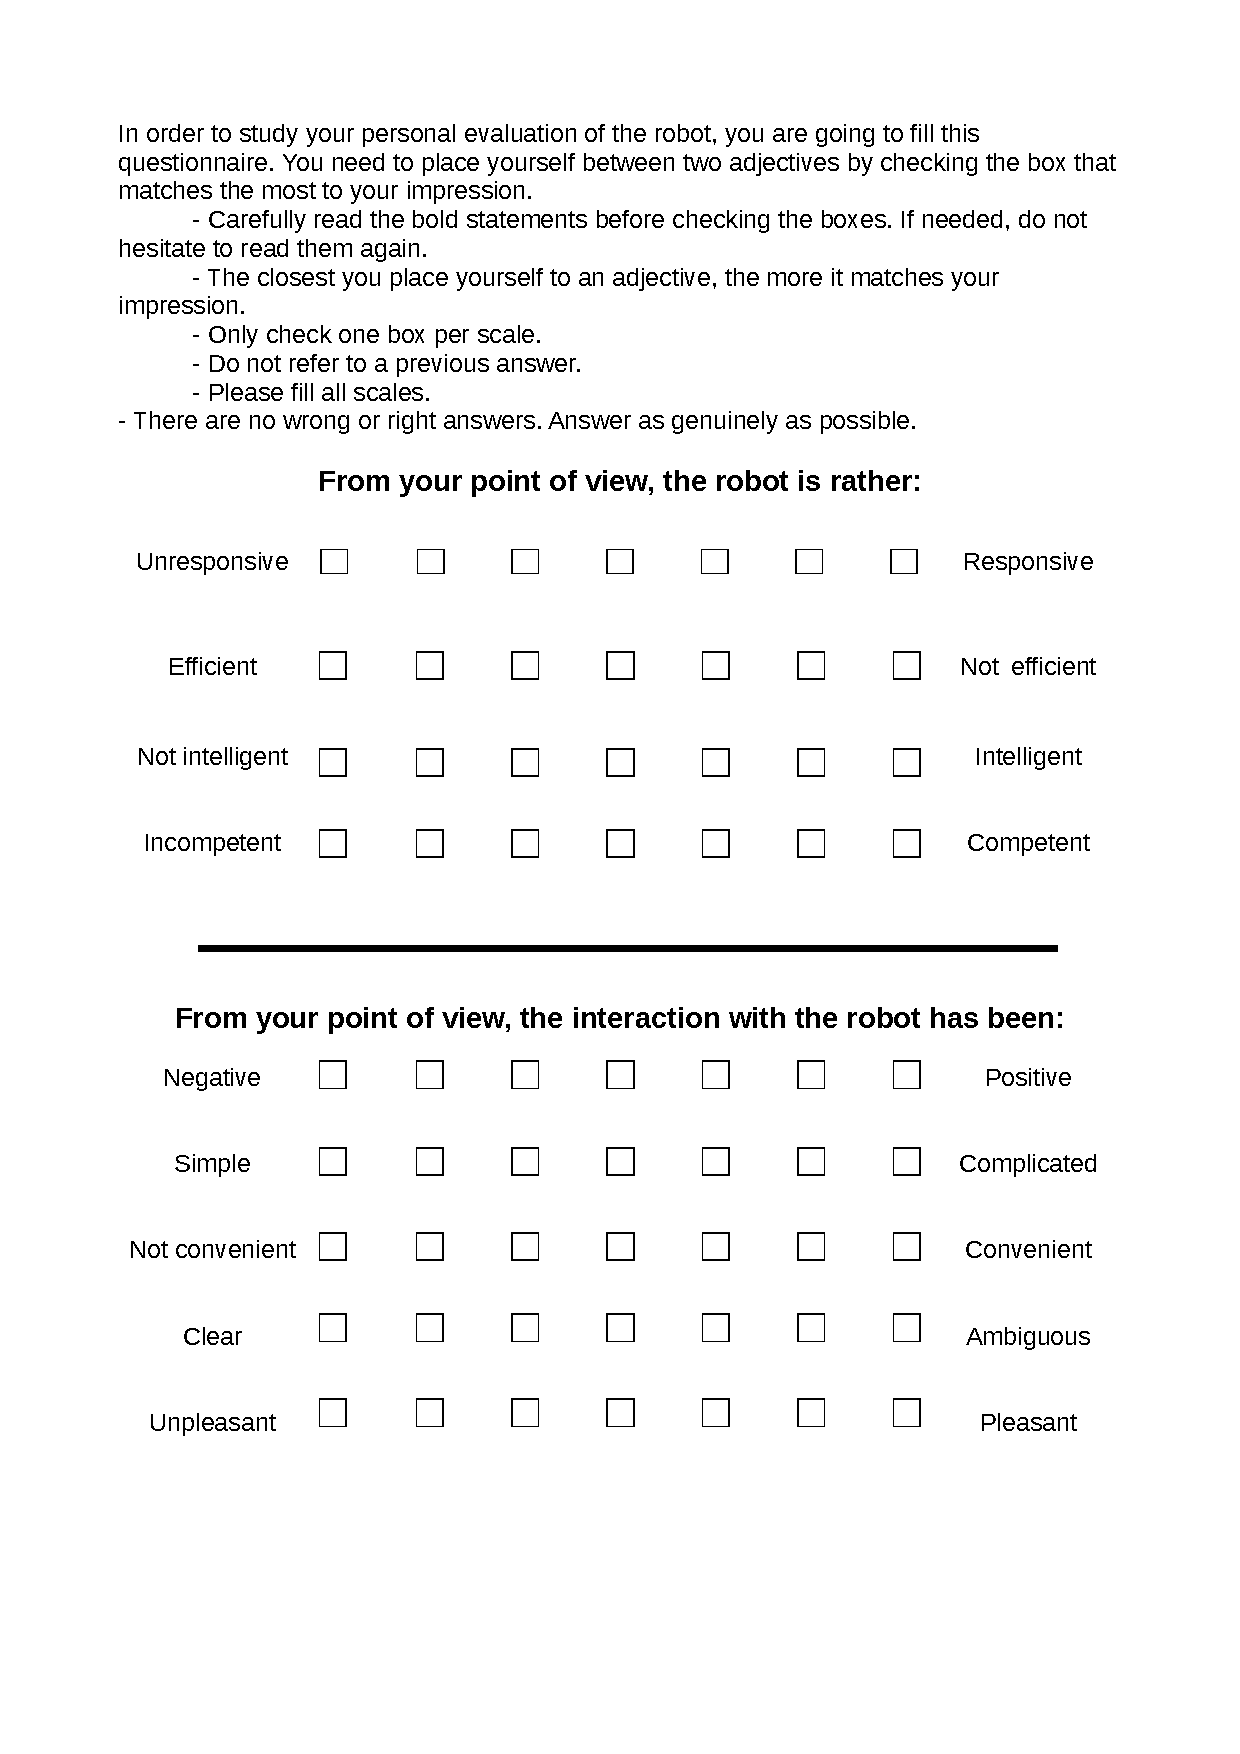
\includegraphics[page=1, width=\textwidth]{Annexes/perdita_translation_en_thesis.pdf} 
\end{center}

\begin{center}
\includegraphics[page=2, width=\textwidth]{Annexes/perdita_translation_en_thesis.pdf} 
\end{center}

\section{Situation Assessment Questionnaire (French)}
\begin{center}
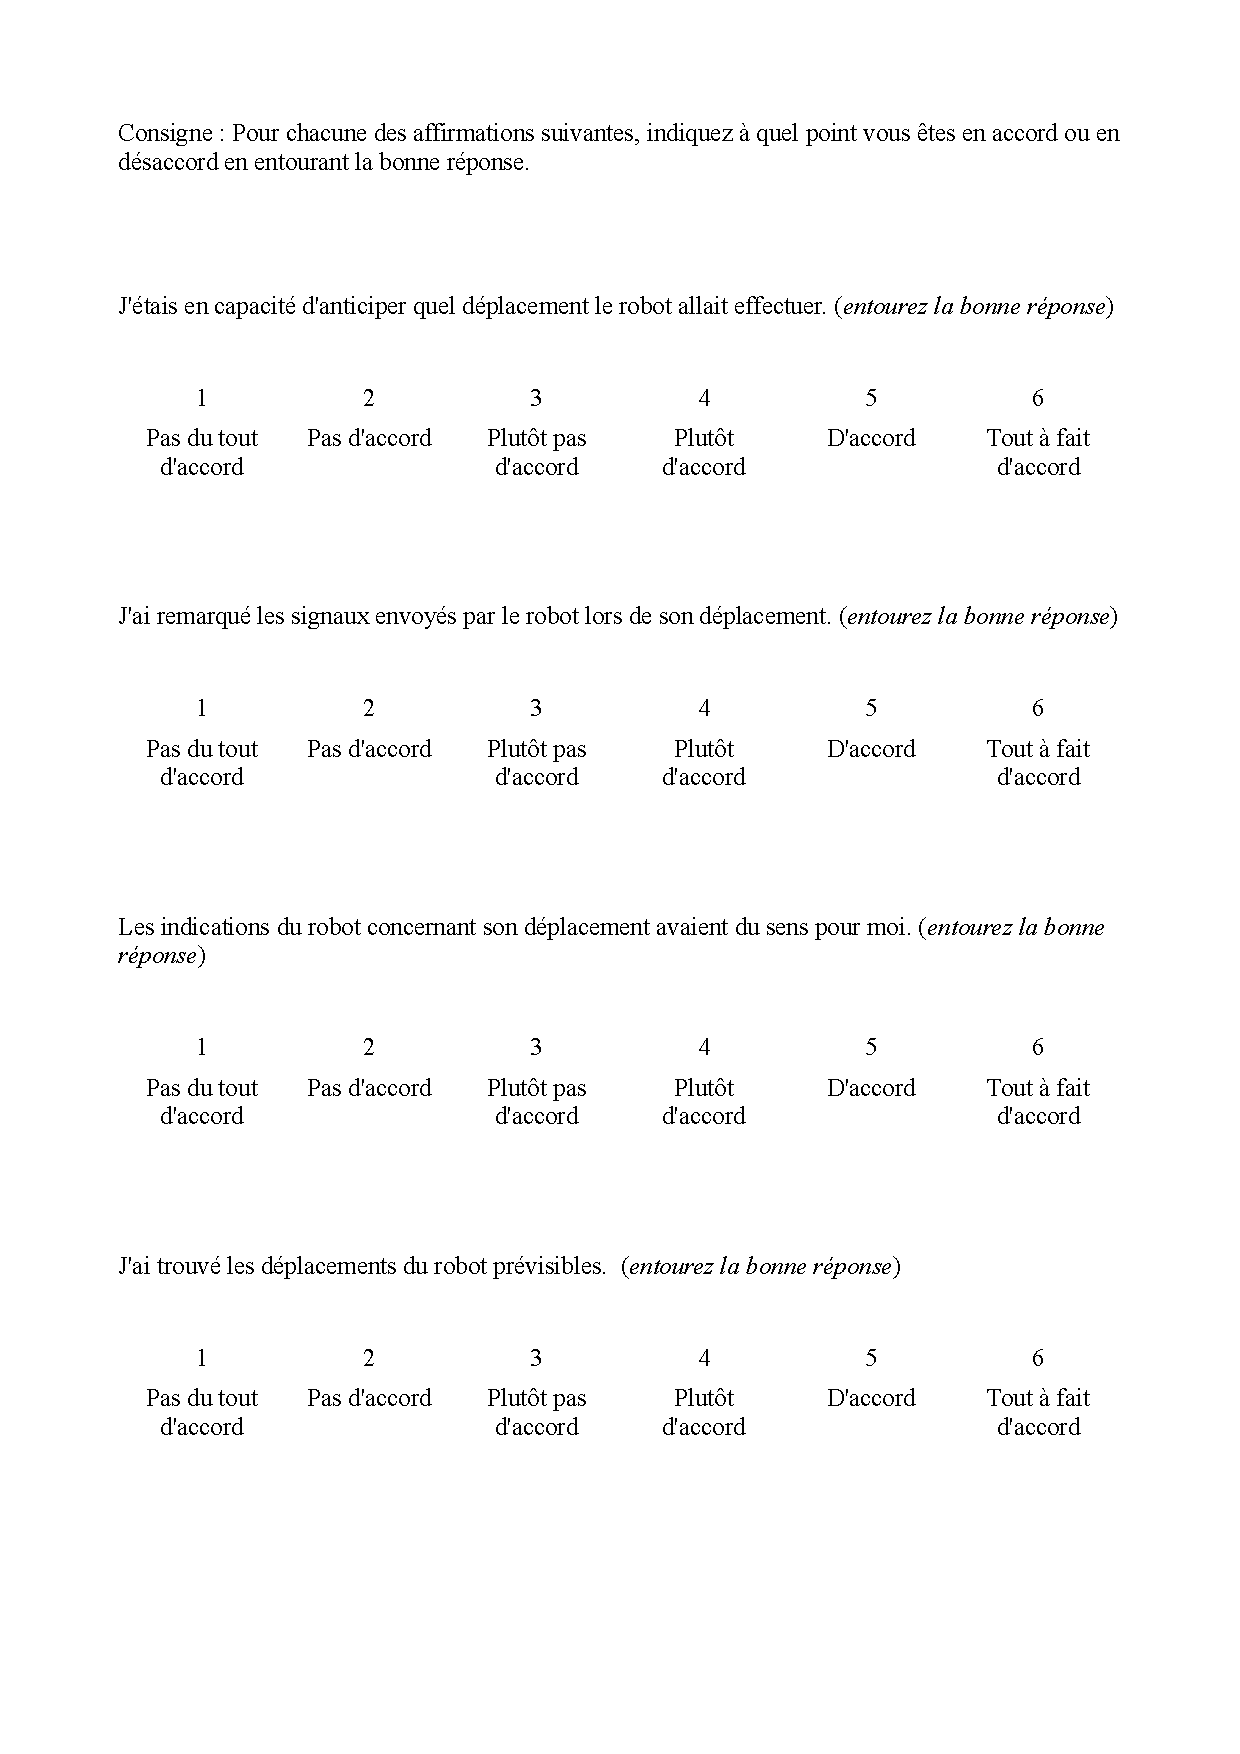
\includegraphics[page=1, width=\textwidth]{Annexes/SAQuestionnaireFr.pdf} 
\end{center}

\begin{center}
\includegraphics[page=2, width=\textwidth]{Annexes/SAQuestionnaireFr.pdf} 
\end{center}

\section{Translation of Situation Assessment Questionnaire Items}
\begin{itemize}
\item J'ai perçu les éléments pertinents indiquant les déplacements du robot.

I perceived the relevant elements indicating the robot motion.

\item J'ai remarqué les signaux envoyés par le robot lors de son déplacement.

I noticed the signals sent by the robot during its motion.

\item J'ai compris le comportement de déplacement du robot.

I understood the robot motion behavior.

\item Les indications du robot concernant son déplacement avaient du sens pour moi.

The robot signs about its motion made sense to me.

\item J'étais en capacité d'anticiper quel déplacement le robot allait effectuer.

I was able to anticipate which motion the robot was going to do.

\item J'ai trouvé les déplacements du robot prévisibles.

It seemed to me that the robot motions were predicatables.
\end{itemize}

\section{AttrakDiff Questionnaire (French)}
This questionnaire is the official translation of the AttrakDiff questionnaire \cite{lallemand_creation_2015}.

\begin{center}
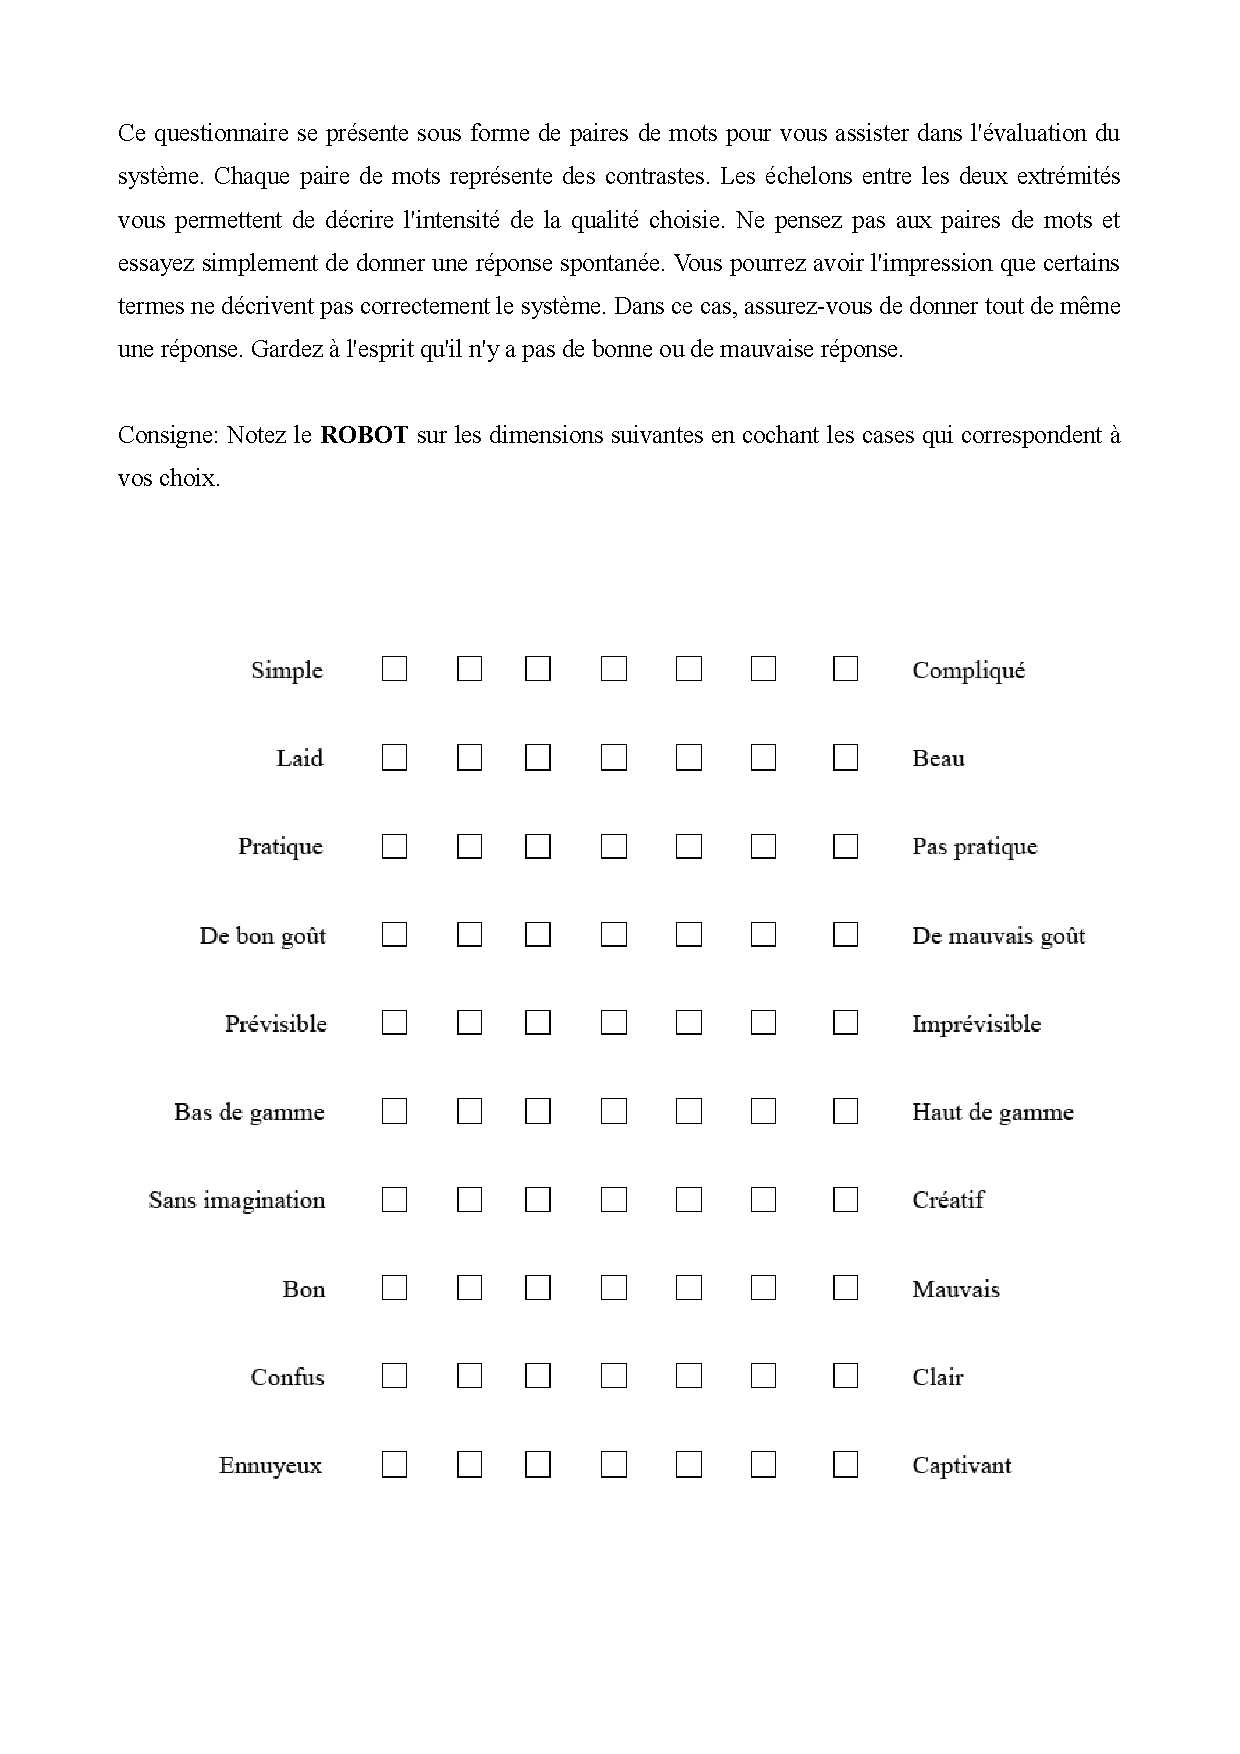
\includegraphics[page=1, width=\textwidth]{Annexes/AttrakDiff.pdf} 
\end{center}





\bibliographystyle{StyleThese}
%\bibliographystyle{plain}
\bibliography{These}

\cleardoublepage
\begin{vcenterpage}
\noindent\rule[2pt]{\textwidth}{0.5pt}

\textbf{Abstract:}
%%%%%%%%%%%%%%%%%%%%%% ATTENTION GUILHEM ! SI MODIFICATION => MODIF SUR ADUM AUSSI !!!
Robots are capable to handle autonomously more and more complex tasks. However, today's robots have either their workspaces are physically separated from the humans ones or their abilities severely restricted when evolving nearby humans. In this thesis, we propose several approaches allowing to plan not only for the robot but also for the human, enabling to predict and elicit their decision process and actions, leading to better human robot interactions (HRI). 

First, we show through a user study, why such a scheme applied to robot navigation is crucial for efficient and satisfactory interaction. Planning for the robot and the human allows to find solution in intricate situations where collaboration is necessary but also for the robot to be proactive and legible while navigating. Secondly, we alleviate from inherent ephemeral nature of interaction in collaborative navigation to explore how co-planning can be applied for task planning. We introduce a new referring expression generation algorithm, working on an ontology as knowledge base, and show that it is the fastest one to date while being designed for HRI application. We use it in a human-aware task planner to estimate feasibility and cost of communication during task planning, preventing deadlock or suboptimal plans. Finally, a novel approach to human-aware task planning is proposed where action models of the robot and the human are distinct and used to produce conditional plans.
\begin{comment}
As technology progresses, more and more complex tasks can be automated. However, robots seldom consider the nearby humans in their decision making processes. This result in today robots usage to be separated from human environment or to be overdefensive when evolving close to humans. We claim that bringing the robot and the human workspace closer would allow to use their complementarity to perform more complex tasks in collaboration, more efficiently and with more satisfaction for the human.

In this thesis we show why it is crucial for a robot not only to plan for itself but also for the nearby human in order to predict, elicit and guide human decisions and actions. 
First, we prove, through a user study, planning both for the robot and the human trajectories is important to make a successful and efficient crossing with a human in a narrow corridor. The resulting robot trajectory are not only more acceptable to the human but also allows for the robot to communicate about the proposed collaborative plan.
Secondly, we alleviate from inherent complexity and ephemeral nature of collaborative motion planning to propose a method for planning communication in human robot task planning. An novel approach for referring expression generation is described and shown to be the most computationally efficient method to date while being designed for human robot interaction scenarios. This algorithm is then integrated in a human robot task planner: the Hierarchical Agent-base Task Planner (HATP), enabling for the estimation of the feasibility and the cost of communication actions by resolving their content during task planning. 
%This require to plan for both robot and human actions while also keeping track of both agents beliefs while planning. Consequently, it prevents deadlocks and results in more efficient plan than if communication actions were resolved during execution.
Finally, we introduce a new task planning scheme reasoning on separate human and robot beliefs and action domains. By exploring two HTNs corresponding respectively to the planning domain of the robot and the task model of the human, the planner is able to predict and elicit human actions by emulating their decision and reaction processes. The pertinence of the scheme is showed on example and a more complete challenging task is presented: the director task.
\end{comment}

\textbf{Résumé :}
%%%%%%%%%%%%%%%%%%%%%% ATTENTION GUILHEM ! SI MODIFICATION => MODIF SUR ADUM AUSSI !!!
Les robots sont capables d'effectuer de manière autonome des tâches toujours plus complexes. Cependant, ils sont encore soit utilisés avec une séparation physique des humains, soit limités lorsqu'ils évoluent proches d'humains. Dans cette thèse, nous proposons plusieurs approches visant à planifier pour le robot mais aussi pour l'humain. Les plans alors générés prennent en compte l'humain en prédisant et provoquant leur actions, menant à de meilleures interactions humains-robots.

Premièrement, nous montrons au travers d'une étude utilisateur, pourquoi une telle approche appliquée à la navigation est cruciale pour une interaction efficiente et satisfaisante. Planifier pour le robot et l'humain permet en effet de trouver des solutions dans des situations d'interaction complexes mais aussi au robot d'avoir un comportement plus lisible et proactif. Deuxièment, nous présentons un algorithme de génération d'expression de référencement, le plus rapide aujourd'hui et pensé pour l'interaction humain-robot. Nous utilisons ensuite cet algorithme pour estimer la faisabilité et le coût des actions de communication pendant la planification de tâches, permettant d'éviter des impasses et des plans sous optimaux. Enfin, nous proposons une approche novatrice à la planification de tâches humain robot, dans laquelle les modèles de l'action des deux agents sont distincts et utilisés pour produire des plans conditionels.

\textbf{Keywords:}

\textbf{Mots clés :}
mots, clefs
\\
\noindent\rule[2pt]{\textwidth}{0.5pt}
\end{vcenterpage}

\end{document}
